% =====================================================================
%  PROTOCOLE TRIADE v0.8.4 — Manuscrit de spécification
%  Corps du document : Tectonic via pdf.py convert.latex.
%  Couverture générée séparément (cover.html, Template 03) et fusionnée
%  en amont — AUCUNE page de titre ici. Le sommaire est la première page
%  du corps.
%  Chaîne née spec_v040 → spec_v050 (D25/D44) → spec_v051 (D75) →
%  spec_v052 (D81) → spec_v060 (D133 — passation du programme de
%  souveraineté cryptographique accompli : axes 2-3-4 livrés et prouvés
%  terrain, axe 1 TEE consigné comme exigence) → spec_v061 (D137 — le
%  niveau de naissance d'un coffre neuf devient l'arbitrage du
%  développeur : CF1/CF2/CF3 à la création ; erratum typographique
%  « tbp] » réparé au passage) → spec_v070 (D169 — la consolidation du
%  programme d'après M7 : M8 le domaine `sys` franchi [finale 0.9.0],
%  M9 le domaine `tls13` ouvert [couche I complète], le sceau à
%  TREIZE arbres, les cérémonies d'ère au protocole) → spec_v080
%  (D176 — la consolidation du programme d'après M9 : le domaine
%  `tls13` FRANCHI [finale 1.0.0, la session réelle], le test
%  grandeur nature ouvert [M10 « Loupe », la notation 18/18], la
%  dette du quatorzième arbre nommée — la cérémonie d'ère du TGN
%  précède tout build) → spec_v081
%  (la révision de terrain du TGN : la cérémonie d'ère PASSÉE
%  SUR PIÈCES [quatorze arbres, la dette soldée], le build
%  loupe 0.1.0-dev.1 NÉ, le terrain a REFUSÉ dev.1 PUIS dev.2
%  du même refus 0xc000007b [l'oubli du BASERELOC, puis la table
%  nécessaire mais PAS suffisante], LA RETOUCHE dev.3 ramène
%  l'image dans l'enveloppe prouvée de la lignée ET le kit porte
%  SA CASCADE DIAGNOSTIQUE — le VRAI chargeur nommera l'axe) →
%  spec_v082 (LA SECONDE RÉVISION DE TERRAIN : LE VRAI CHARGEUR A
%  CARTOGRAPHIÉ dev.3 — la première fois au terrain, l'enveloppe
%  PROUVÉE — puis LE TÉMOIN A NOMMÉ AU T0 [CADRE-NÉ] : l'initialiseur
%  du build avait posé le sentinel à +8 [une TAILLE prise pour un
%  offset] au lieu de +528 [la chaîne des tailles du plan] ; LA
%  RETOUCHE dev.4 fait de l'initialiseur .data LE MIROIR EXACT du
%  CADRE_VIERGE du harnais ET LE GARDE EST GUÉRI — le validateur
%  relit LE MÊME miroir : le contrôle dérive du plan, jamais de la
%  pièce qu'il contrôle — et le scénario relit LE .data ENTIER
%  contre le miroir).
% =====================================================================
\documentclass[11pt,a4paper]{article}

% ---------- Polices ----------
\usepackage{fontspec}
\setmainfont{Liberation Serif}
\setsansfont{Liberation Sans}
\setmonofont{Liberation Mono}
\usepackage[french]{babel}
\addto\captionsfrench{\renewcommand{\tablename}{Tableau}}

% ---------- Mathématiques ----------
\usepackage{amsmath,amssymb,amsthm}

% ---------- Mise en page ----------
\usepackage{geometry}
\geometry{a4paper, top=2.4cm, bottom=2.4cm, left=2.2cm, right=2.2cm, headheight=14pt}
\usepackage{graphicx}
\usepackage{xcolor}
\definecolor{liaison}{HTML}{3681A6}
\definecolor{grisdoux}{HTML}{555F66}
\usepackage{booktabs}
\usepackage{tabularx}
\newcolumntype{Y}{>{\raggedright\arraybackslash}X}
\usepackage{multirow}
\usepackage{longtable}
\usepackage[export]{adjustbox}
\usepackage{enumitem}
\setlist{noitemsep, topsep=2pt, leftmargin=1.4em}
\usepackage{microtype}

% ---------- Théorèmes ----------
\theoremstyle{definition}
\newtheorem{regle}{Règle}

% ---------- Listings ----------
\usepackage{listings}
\lstset{
  basicstyle=\footnotesize\ttfamily,
  keywordstyle=\bfseries,
  commentstyle=\itshape\color{grisdoux},
  breaklines=true,
  showstringspaces=false,
  columns=fullflexible,
  keepspaces=true,
  frame=single,
  framerule=0.3pt,
  rulecolor=\color{black!25},
  xleftmargin=4pt, xrightmargin=4pt,
  aboveskip=6pt, belowskip=6pt,
}

% ---------- Titres ----------
\usepackage{titlesec}
\titleformat{\section}
  {\Large\sffamily\bfseries\color{liaison}}{\thesection}{0.6em}{}
\titleformat{\subsection}
  {\large\sffamily\bfseries}{\thesubsection}{0.6em}{}
\titlespacing*{\section}{0pt}{14pt plus 4pt minus 2pt}{7pt plus 2pt minus 2pt}

% ---------- En-têtes / pieds ----------
\usepackage{fancyhdr}
\pagestyle{fancy}
\fancyhf{}
\fancyhead[L]{\small\itshape Protocole TRIADE — spécification v0.8.4}
\fancyfoot[C]{\small\thepage}
\renewcommand{\headrulewidth}{0.3pt}

% ---------- Divers ----------
\raggedbottom
\emergencystretch=3em
\widowpenalty=10000
\clubpenalty=10000
\setcounter{tocdepth}{2}

% hyperref : TOUJOURS en dernier
\usepackage[colorlinks=true, linkcolor=liaison, citecolor=grisdoux,
            urlcolor=liaison, bookmarks=true, bookmarksnumbered=true,
            unicode=true]{hyperref}

\hypersetup{
  pdftitle={Protocole TRIADE v0.8.4 — spécification technique},
  pdfauthor={Alexis FR-LOPEZ ; Agent Z.ai (GLM)},
  pdfsubject={Gouvernance vérifiable du développement logiciel assisté par IA},
  pdfkeywords={TRIADE, agent-first, contrat, vérification, gouvernance, profils, souveraineté cryptographique, coffre-fort}
}

\newcommand{\code}[1]{\texttt{#1}}

\begin{document}

% Le sommaire est la première page du corps (la couverture est fusionnée
% en amont). Conformité avec la règle « TOC = première page ».
\tableofcontents
\newpage

% =====================================================================
%  CH 1-4 : Vision · Couche I et taxonomie · Couches et traçabilité · Carte
% =====================================================================
\section{Vision et objectifs}\label{sec:vision}

Le développement logiciel est entré dans l’ère \emph{agent-first} : une part croissante du
code est écrite, relue et modifiée par des modèles de langage plutôt que par des humains.
Cette bascule remet en question une hypothèse centrale de nos outils — que le code source
est optimisé pour la lecture humaine. TRIADE est la réponse disciplinée à ce réexamen :
plutôt que de supprimer les langages (une impossibilité de principe, puisqu’un modèle de
langage manipule des symboles textuels et que tout format binaire rendu lisible par un
agent constitue de facto un langage), TRIADE déplace le langage vers une fine couche de
spécification maintenue par l’agent, tandis que l’artefact livré est du code machine natif
pur. Le compilateur disparaît du pipeline de livraison : ce que l’agent écrit est ce qui
s’exécute — et rien d’autre.

Le nom encode l’architecture : trois couches indissociables — Intention (I), Binaire (B),
Carte (C) — unies par un verrou croisé cryptographique. La couche I contient le quoi et le
pourquoi : contrats typés, pré et post-conditions, invariants, cas d’échec, vecteurs de
vérification. La couche B contient le comment : des octets scellés, versionnés, à adresses
stables. La couche C est l’index naviguable qui lie les deux et sert d’unique interface de
développement à l’agent.

La v0.4.0 tire les enseignements de la première validation à l’échelle — le recodage
complet de RoomEq (démonstration v0.3) — et les convertit en normes : ce que la
démonstration a pratiqué (reverse-specs, pré-versions, partage de fixtures, mesure avant
optimisation) devient exigence ; ce que son analyse des défauts a révélé devient
taxonomie ; ce que son étude de cas établit et ne prouve pas reste explicitement hors
périmètre de preuve.

La v0.5.0 est la révision du retour du terrain. Les jalons M0 (chaîne artefact), M1
(mini-libc scellée) et M2 (patch à chaud en production, avec retour arrière) sont
franchis — chacun sur validation terrain Windows 11, chacun scellé par une balise
finale immuable (0.2.0, 0.3.0). La campagne M2 a coûté huit classes de défauts
invisibles à l’émulation (§\ref{sec:taxonomieX}) — le prix d’une leçon : un oracle
valide un artefact contre un modèle d’environnement, et la complétude du modèle ne se
démontre qu’en exécutant le binaire sur le système réel. Ce que le terrain a appris
devient norme : la boucle d’évidence (§\ref{sec:terrain}), la taxonomie X,
l’instrumentation contractualisée — et l’ouverture du jalon M3, contrats renforcés
sur entrées non fiables.

\subsection{Fonction objectif hiérarchisée — invariant de révision}\label{sec:objectif}

\begin{center}
\large\bfseries Sécurité $>$ Performance $>$ Optimisation $>$ Coût en tokens
\end{center}

\medskip

Arbitrage lexicographique : un objectif n’est jamais sacrifié au profit d’un objectif de
rang inférieur. La v0.4.0 consigne cette hiérarchie comme \textbf{invariant de révision}
(D19) : aucune révision future du protocole ne peut la modifier sans invalider
explicitement le protocole entier — pas l’ordre, pas les rangs, pas la non-compensation.

\begin{table}[htbp]
\centering\small
\caption{La fonction objectif et ses métriques de validation.}
\label{tab:objectif}
\begin{tabularx}{\textwidth}{@{}l Y Y@{}}
\toprule
\textbf{Objectif} & \textbf{Signification concrète} & \textbf{Métrique de validation} \\
\midrule
Sécurité & Sûreté mémoire validée par oracle ; intégrité carte $\leftrightarrow$ binaire ;
durcissement au chargement & 0 corruption détectée ; tout échec de verrou bloque la
session ; échec au lancement = arrêt propre \\
Performance & 100 \% code machine natif ; zéro abstraction intermédiaire &
Comparaison par bloc scellé face à une référence compilée \\
Optimisation & Descente à l’ISA sur hot paths identifiés — jamais sans mesure (R11) &
Gain mesuré et journalisé par bloc optimisé \\
Coût en tokens & Édition ciblée via la carte ; jamais de lecture intégrale du binaire &
Budgets par type d’opération (§\ref{sec:carte}) \\
\bottomrule
\end{tabularx}
\end{table}

\subsection{Périmètre et non-objectifs}\label{sec:perimetre}

Cinq non-objectifs. Premièrement, TRIADE ne prétend pas remplacer les langages dans
l’industrie : c’est une architecture de laboratoire. Deuxièmement, la furtivité face aux
EDR n’est pas recherchée : l’outil cible est un utilitaire de pentest pour tests autorisés
en laboratoire, appelant les API du système via les interfaces standards du profil.
Troisièmement, l’universalité est structurelle mais progressive : chaque profil doit être
instancié et validé (M6, M7) avant d’être déclaré supporté — le protocole ne promet pas la
portabilité, il la vérifie. Quatrièmement, aucune couche d’abstraction à l’exécution
(bytecode portable, machine virtuelle, traduction à la volée) n’est introduite : elle
trahirait la fonction objectif Performance. Cinquièmement, la couche de gouvernance
validée par la démonstration et le cœur natif du protocole (notation, verrou
cryptographique sur octets, patch à chaud) restent des niveaux de preuve distincts : les
jalons M0 à M7 demeurent la charge de validation du cœur natif.

\subsection{Ce que change la v0.4.0}\label{sec:nouveautes}

Dix-sept évolutions, toutes tracées dans la correspondance du §\ref{sec:correspondance} et
dans le journal des versions, toutes rattachées aux décisions D19 à D24 : normalisation de
la couche I, taxonomie des défauts, traçabilité I $\leftrightarrow$ C $\leftrightarrow$
B $\leftrightarrow$ tests, norme de fragmentation, localisation par intention, R10
renforcée, R11 nouvelle, suite de conformité par profil, parité inter-profils,
pré-versions, reverse-specs, journal d’optimisation, modèle de menace étendu, journal des
décisions normalisé, tableau de bord de conformité. Aucune règle existante n’est
affaiblie ; aucune couche n’est ajoutée à l’exécution ; la hiérarchie de la fonction
objectif est inchangée.

\subsection{Ce que change la v0.5.0}

Huit évolutions, toutes tracées dans la correspondance (§\ref{sec:evolutions050}) et le
journal des versions, toutes rattachées aux décisions D26 à D45 : la validation
terrain devient une couche de vérification normée — boucle d’évidence, journal
d’exécution, instrumentation contractualisée, diff chirurgical (§\ref{sec:terrain}) ;
la taxonomie des défauts s’étend des classes T (contrat non écrit) aux classes X —
défauts invisibles à l’émulation, huit classes nommées par la campagne M2
(§\ref{sec:taxonomieX}) ; l’état des jalons est constaté — M0, M1 et M2 franchis sur
validations terrain Windows 11, balises finales 0.2.0 et 0.3.0 posées
(§\ref{sec:jalons}) ; le budget de localisation est corrigé à 64 tokens (D31) et les
budgets affichent leurs valeurs mesurées ; les volumes d’oracle effectifs sont
consignés ; les preuves terrain sont archivées brutes avec leurs empreintes ; le
corpus de démonstration (huit itérations instrumentées) devient l’occurrence de
référence de la méthode ; le jalon M3 est ouvert — contrats renforcés sur entrées non
fiables et fuzzing à propriétés (D45). Aucune règle n’est modifiée ; aucune couche
n’est ajoutée à l’exécution ; la hiérarchie de la fonction objectif est inchangée.

\subsection{Ce que change la v0.5.1}\label{sec:nouveautes051}

Un composant nouveau et deux constats, tous tracés dans la correspondance
(§\ref{sec:evolutions051}) et le journal des versions, rattachés à la décision D75 : le
\textbf{coffre-fort des phrases maîtresses} — conteneur chiffré TRIADE-CF1 centralisant
toutes les phrases maîtresses par projet, sur la pile cryptographique de la carte au
repos (Argon2id aux planchers, HKDF à contexte dédié, XChaCha20-Poly1305), doté d’un
autotest de falsification et de règles d’export/import (continuité,
§\ref{sec:gouvernance} ; FORMAT\_CARTE § 11) ; l’état des jalons est constaté — M3
franchi le 28 octobre 2026 sur la campagne million (D72), la conformité permanente
(D73) et le scellage de la balise finale 0.4.0 (D74) ; le modèle de menace gagne la
ligne du vol du coffre-fort (§\ref{sec:menaces}). Aucune règle n’est modifiée ; aucune
couche n’est ajoutée à l’exécution ; la hiérarchie de la fonction objectif est inchangée.

\subsection{Ce que change la v0.5.2}\label{sec:nouveautes052}

Une évolution de discipline, tracée dans la correspondance (§\ref{sec:evolutions052}) et
le journal des versions, rattachée à la décision D81 : la \textbf{phrase de contrôle du
coffre-fort passe sous garde durable} — dès sa production (init, rotation,
changement), elle est sauvegardée dans le dépôt git (commit dédié, push GitHub, miroir
du coffre Drive par le hook) et au racine du coffre Drive \emph{avant} toute autre action
de la session ; le fichier \code{PHRASE-CONTROLE-COFFRE.txt} (phrase seule sur une
ligne, lisible tel quel par \code{--phrase-fichier}) \emph{est} la remise — l’affichage
unique de cérémonie (D27/D30) cesse d’être le canal de survie. Le constat fondateur : la
rotation D80 avait produit une phrase neuve dont la remise prévue en fin de tour n’a
jamais eu lieu — la session d’exécution est morte avant (pannes d’infrastructure
récurrentes) — et la phrase ne vivait plus que dans le bac à sable éphémère : un décès
d’infra de plus et le coffre entier devenait indéchiffrable à jamais. L’arbitrage est
consigné : le risque de \textsc{perte} (vécu, répété) est jugé supérieur au risque
d’\textsc{exposition} (URL non devinable) ; le modèle de menace en tire la conséquence
honnête — la confidentialité des phrases au repos repose désormais sur le contrôle
d’accès au dossier du coffre Drive, la mitigation première devient la restriction du
partage par lien, et une phrase entrée dans l’historique git y demeure à vie : on ne
compte plus sur sa confidentialité, la rotation reste le remède. L’état des jalons est
constaté — M4 ouvert le 28 octobre 2026 (D77, couche I écrite-avant-code : huit
spécifications \code{tls} et deux révisions \code{http}). Aucune règle n’est modifiée ;
aucune couche n’est ajoutée à l’exécution ; la hiérarchie de la fonction objectif est
inchangée.

\subsection{Ce que change la v0.6.0}\label{sec:nouveautes060}

La révision de génération attendue par le plan : le \textbf{programme de souveraineté
cryptographique est accompli et prouvé sur terrain} — décision de passation D133,
arbitrage du développeur. Trois axes livrés (§\ref{sec:souverainete}) : l'\textbf{axe 2}
(D86) — le coffre CF2 à clé maîtresse répartie par Shamir, cinq gardes seuil trois,
sentinelle à double seuil puis PORTE D120 ; l'\textbf{axe 3} (D87) — le sceau de
l'Intention : dix arbres de couche I signés par la clé Ed25519 hors-ligne du
développeur, gardes de build et de patch ; l'\textbf{axe 4} (D121, né du terrain) — le
coffre CF3 : la serrure à triple scellement, le piège sur média séparé, la sentinelle
instantanée \emph{par invocation} et le cycle en deux actes. L'\textbf{axe 1} (D85,
attestation TEE) demeure une exigence consignée : l'infrastructure sans racine de
confiance matérielle ne peut pas la satisfaire et le dit. La \textbf{chaîne réelle du
coffre} a migré sur le terrain du développeur les 30--31 octobre 2026 — CF1 vérifié
INTÈGRE, phrase de contrôle changée (D110), CF2 migré (cinq gardes, seuil 3, trois
copies hors-ligne), CF3 migré (époque 1, checksum \code{0cc89a96}), verdict à froid
VERT deux fois — les cérémonies étant conduites par le maître de cérémonie graphique
(D107--D118) avec le kit Drive tenu identique au miroir par construction (D130). Un
\textbf{coffre neuf naissait CF3} : \code{init} direct à l'époque 1 — la chaîne
de migration est l'histoire du coffre réel, pas un rite obligé (la v0.6.1 remet ce
choix au développeur — §\ref{sec:nouveautes061}, §\ref{sec:initniveau}). Un document
complémentaire, le \emph{Livre du Coffre} (même date, même dépôt), porte la posture
opératoire du maître : cérémonies pas à pas, runbook, mode dégradé. Aucune règle du
cœur n'est modifiée ; aucune couche n'est ajoutée à l'exécution ; la hiérarchie de la
fonction objectif est inchangée.

\subsection{Ce que change la v0.6.1}\label{sec:nouveautes061}

Une seule règle, explicitement invalidée et remplacée (§\ref{sec:evolutions061}) :
le niveau de sécurité d'un coffre neuf. La v0.6.0 (D133) l'avait fixé — un coffre
neuf naît CF3, \code{init} direct à l'époque 1 ; la v0.6.1 (D137) en fait
\textbf{l'arbitrage du développeur au moment de créer son projet de développement} :
CF1, CF2 ou CF3, chacun avec son acte de naissance, ses obligations et son guide
(§\ref{sec:initniveau}) — imposer CF3 par défaut risque d'être trop contraignant
selon le projet : média du piège à produire dès le premier jour, cycle en deux actes
à chaque session, sachet physique à tenir — la contrainte se justifie quand le secret
la mérite. La chaîne de migration CF1 $\to$ CF2 $\to$ CF3 demeure disponible à tout
moment pour un coffre dont les besoins grandissent ; le coffre réel de TRIADE reste
CF3 (époque 1, checksum \code{0cc89a96}). Aucune autre règle n'est modifiée ; aucune
couche n'est ajoutée à l'exécution ; la hiérarchie de la fonction objectif est
inchangée.

\subsection{Ce que change la v0.7.0}\label{sec:nouveautes070}

La révision de consolidation du programme d'après M7 (D160) : ce que la clôture de la
v0.6.1 tenait « hors périmètre courant » entre dans la spécification, sur résultats
mesurés — la clause est levée NOMMÉMENT pour les deux premières familles, les profils
additionnels demeurent hors périmètre. Le \textbf{jalon M8} (le bloc optionnel de
syscalls directs — le domaine \code{sys}) est franchi : la charte à huit règles (le SSN
est une donnée, jamais un octet de code ; le motif du stub vérifié avant toute
extraction ; un stub divergent est un refus nommé — le résolveur ne devine jamais, il ne
s'adapte jamais en silence), les spécifications sys-01…03 écrites-avant-code, le harnais
différentiel 61 contrôles verts sur fixtures \code{ntdll} synthétiques (le laboratoire
ne connaît jamais le SSN du terrain), la cérémonie de l'ère passée avant le build (12
arbres, D162/D163), le run terrain sur le VRAI \code{ntdll} — la twin de la ligne
hello-02 par les DEUX chemins (l'IAT \code{kernel32} et le syscall direct
\code{NtWriteFile}), le refus $-4$ nommé du stub crocheté — recoupé 30/30 sur pièces
croisées, la finale \code{0.9.0} scellée (Entrée 164, D165 : le scellage exige le
verdict du recoup comme pièce ; le scellage est un fait de carte, l'artefact ne bouge
jamais). Le \textbf{jalon M9} (TLS 1.3 pur en blocs scellés — le domaine \code{tls13},
l'ère 1.0.0) est ouvert (D166) : la couche I complète — 28 spécifications en six
familles (sha, hkdf, x25519, aead, enregistrement, poignée, principal), l'instrument
\code{verifier\_specs\_m9a.py} 117 contrôles verts (D167) — et la cérémonie de l'ère
passée le 05/11 : la remise du développeur, TREIZE arbres signés hors ligne à la clé du
04/11 (la continuité prouvée par le déterminisme Ed25519, D163 : les onze arbres
inchangés rendent les signatures de l'ère M8), le garde repassé VERT 13/13 — la dette
D166 soldée sur pièces. Le \textbf{sceau de l'Intention} porte désormais treize arbres
(§\ref{sec:sceauI}) et les cérémonies d'ère entrent au protocole
(§\ref{sec:ceremoniesere}) : la dette se nomme à la naissance, jamais après coup (D166,
règle 8) ; la charge se prépare au geste qui sert la main du développeur (D168). Aucune
règle du cœur n'est modifiée ; aucune couche n'est ajoutée à l'exécution ; la hiérarchie
de la fonction objectif est inchangée.

\subsection{Ce que change la v0.8.0}\label{sec:nouveautes080}

La révision de consolidation du programme d'après M9 (D170/D171). Le \textbf{jalon M9}
(TLS 1.3 pur en blocs scellés — le domaine \code{tls13}, l'ère 1.0.0) est franchi : les
28 blocs notés-mesurés-prouvés — les primitives aux vecteurs officiels octet pour octet
(FIPS 180-4, RFC 2104/4231, 5869, 7748, SP 800-38D), la poignée rejouée sur le
transcript RFC 8448, les héritages PAR LA CARTE (R7) —, le socle socket par syscalls
directs, le septième run terrain vert sur pièces et recoupé 34/34, LA SESSION RÉELLE
(la ligne applicative chiffrée ÉCHANGÉE avec un serveur réel, le témoin
« HTTP/1.1 200 OK » DÉCHIFFRÉ PAR LA MACHINE, l'épinglage $-6$ NOMMÉ contre le vrai
serveur, la fermeture propre), la finale \code{1.0.0} scellée sur le recoup exigé
comme pièce (D170 : le scellage est un fait de carte, l'artefact ne bouge jamais) — et
l'ère M8 refermée propre par l'export de continuité. \textbf{LE TEST GRANDEUR NATURE
est ouvert (D171)} : le protocole avait prouvé chaque capacité, M0 à M9 — il reste à
prouver qu'il DÉVELOPPE une application réelle NEUVE, de l'intention à l'octet livré
(le modèle RoomEq s'arrêtait au recodage ; le TGN exige la CRÉATION). L'application —
arbitrée à D171, contredisable — est « Loupe », l'éditeur hexadécimal au panneau
d'empreintes sur le profil primaire (l'outil du quotidien du projet : voir les octets,
leurs lignes, leurs empreintes md5/sha-256, leur place) : le domaine \code{loupe}
fondé (la charte + le tableau des 18 blocs en cinq familles), la couche I posée
écrite-avant-code (D172 : les 18 spécifications, le plan d'adressage arrêté avant
toute notation, la table des sept verdicts), et les QUATRE chantiers de notation
accomplis — le noyau fichier + empreintes (D173 : les héritages vivent à leurs
adresses scellées, le mini-OS virtuel du harnais), le rendu + la navigation (D174 :
l'oracle à scénarios — l'écran attendu octet par octet —, le mini-GUI virtuel, le
plancher qui ne recule jamais), l'édition + la table de routage étendue de loupe-09
r2 (D175 : le disque saisissable et la mort du harnais, le réseau de la garde
16$\leftrightarrow$17$\leftrightarrow$18, l'écriture à l'octet prouvée différentielle) —
les 18 blocs NOTÉS-MESURÉS-PROUVÉS, 45 + 53 + 59 contrôles verts aux trois graines sur
les trois harnais. \textbf{L'ère du TGN est OUVERTE AU BUILD} (v0.8.1, la révision de
terrain) : LA CÉRÉMONIE D'ÈRE est PASSÉE SUR PIÈCES — le garde à QUATORZE arbres
verts, la dette D166/D171 SOLDÉE, la remise du développeur INSTALLÉE au coffre
(§\ref{sec:ceremoniesere}) — le build \code{loupe.exe 0.1.0-dev.1} est NÉ, la carte
génération 13, le verrou croisé 26/26. \textbf{ET LE TERRAIN A DIT TROIS FOIS,
CHAQUE REFUS NOMMÉ} (v0.8.2) : le run M10-(e) a REFUSÉ dev.1 par le VRAI
chargeur Windows — 0xc000007b au geste de cartographie (LoadLibraryEx
DONT\_RESOLVE : l'image ASLR sans table de relocalisation, l'oubli nommé du
premier build) — puis dev.2 DU MÊME REFUS (le BASERELOC rendu était NÉCESSAIRE
mais PAS SUFFISANT) : la preuve par la lignée isole les axes par lesquels
l'image sortait de l'enveloppe des HUIT artefacts passés au terrain (le trou de page
0x3000-0x4000, le BSS massif \code{.data} VS~$\gg$~RS, le sous-système GUI) ;
LA RETOUCHE dev.3 ramène l'image DANS l'enveloppe prouvée (.rdata étendue 0x2000 :
plus aucun trou ; .data VS~$=$~RS : plus aucun BSS — AUCUNE adresse scellée ne
bouge), ET LE KIT PORTE SA CASCADE DIAGNOSTIQUE. \textbf{LE RUN REJOUÉ A ÉTÉ LE
PAS DÉCISIF (l'Entrée 206) : LE VRAI CHARGEUR DE WINDOWS A CARTOGRAPHIÉ L'IMAGE —
la première fois au terrain, l'enveloppe prouvée DEMEURE NORME DE FAIT — puis LE
TÉMOIN A NOMMÉ AU T0 [CADRE-NÉ]} : le CADRE \code{.data} n'était pas né poignée
INVALIDE, l'initialiseur du build avait posé le sentinel à +8 (UNE TAILLE
\code{CADRE\_POIGNEE} prise pour un offset) au lieu de +528 (la chaîne des
tailles du plan — le zéro aurait été UNE SESSION FANTÔME au premier \code{ouvrir()}) ;
LA RETOUCHE dev.4 fait de l'initialiseur \code{.data} LE MIROIR EXACT du
\code{CADRE\_VIERGE} du harnais (l'offset CALCULÉ, jamais gravé de tête) ET LE
GARDE EST GUÉRI : le validateur du build validait à +8 — la même constante
fautive, un garde blessé par le défaut qu'il croyait garder ne garde rien — il
relit désormais LE MÊME miroir (la comparaison ENTIÈRE, le \code{.data} relu à
l'octet près) et le scénario relit LE \code{.data} ENTIER contre le miroir — un
échec nommé vaut plus qu'un vert muet, et le TGN fait exactement ce pour quoi il
existe (§\ref{sec:terrain}). \textbf{LE QUATRIÈME RUN A ÉTÉ LE PAS LE
PLUS LOIN JAMAIS VÊCU — ET LA VITRINE A VÉCU SA PREMIÈRE FOIS} (v0.8.3,
l'Entrée 207) : \textbf{[T0] TOUT VERT au témoin} (l'image cartographiée, LE
CADRE NÉ MIROIR — la retouche de l'Entrée 206 TENUE au terrain, l'IAT 37
feuilles posées) PUIS \textbf{[T1] ÉCHEC NOMMÉ [SESSION]} : loupe-01 a rendu
$-6$ SYSTÈME sur un fichier pourtant relu à l'instant, ET « quand je lance
l'exe, la fenêtre s'ouvre et se referme immédiatement » — LA MORT SANS TÉMOIN.
L'AUTOPSIE SUR LA PIÈCE NOMME \textbf{LA CLASSE DES ARGUMENTS PILE} : les
arguments 5+ de l'ABI msx64 vivaient AU HOME SPACE \code{[rsp..0x18]} au lieu
de \code{[rsp+0x20]+} — le VRAI CreateFileW lisait sa disposition À LA PILE NON
INITIALISÉE (loupe-01) ET le contexte condensé VIVAIT SUR LE VRAI SLOT (loupe-05 :
le VRAI ReadFile lisait H0[0] \code{0x6A09E667…} COMME UN POINTEUR — la mort de
la vitrine avec fichier ; loupe-06 pareil) — POURQUOI LE LABO N'AVAIT RIEN VU :
les shims du harnais ne lisaient AUCUN argument pile (le garde avait déjà la
bonne convention dans le shim TextOutW — elle n'était pas appliquée aux feuilles
du noyau). LA RETOUCHE dev.5 : les TROIS notations à leurs vrais slots, DEUX AXES
D'ALIGNEMENT nommés par L'AUDIT D'ABI msx64 NÉ AU BUILD (loupe-10 le
sous-programme \code{.peindre} appelait TextOutW pile $\equiv 8$ : le VRAI
gdi32 est SSE — l'axe que seul l'audit statique voit ; loupe-11 le cadre
\code{0x38}$\to$\code{0x40}), LE GARDE GUÉRI PAR LA CONVENTION (les shims
relisent LES MÊMES SLOTS QUE LE VRAI — la falsification demandée est attrapée)
ET LE KIT PORTE DÉSORMAIS SON TÉMOIN VITRINE (\code{temoin-vitrine.bat} : les
deux codes de sortie + le rapport WER — la prochaine mort sera nommée).
\textbf{LE CINQUIÈME RUN A NOMMÉ $-7$ VERROUILLÉ — ET LA PIÈCE EST
ACQUITTÉE} (v0.8.4, l'Entrée 208) : l'appel CreateFileW de loupe-01 était
NÉ PARFAIT dans la pièce (rcx = le chemin, rdx = \code{0xC0000000}
[GENERIC\_READ|GENERIC\_WRITE], r8 = 1 [FILE\_SHARE\_READ], les arguments
5/6/7 À LEURS VRAIS SLOTS, la pile $\equiv 0 \pmod{16}$) — LA PREUVE PAR LE
NOM CHANGÉ : dev.4 rendait $-6$ SYSTÈME (gle 87 : l'appel mal né),
dev.5 rend $-7$ VERROUILLÉ (gle 32 : l'appel NÉ, refusé pour une RAISON
RÉELLE) — la classe de l'Entrée 207 A TENU AU TERRAIN ; ET LA RAISON
RÉELLE ÉTAIT LE KIT LUI-MÊME : le scénario EST LE CHARGEUR —
\code{LoadLibraryEx} DONT\_RESOLVE TIENT loupe.exe comme SECTION VIVANTE
(sans partage d'écriture), et le VRAI Windows refuse gle 32 d'ouvrir À
L'ÉCRITURE le fichier d'une image mappée : T1 offrait LA PIÈCE ELLE-MÊME
à l'écriture, IMPOSSIBLE PAR CONSTRUCTION — invisible aux runs
précédents parce qu'aucun appel n'était jamais assez bien né pour
atteindre le partage ; loupe-01 A TRADUIT LE REFUS AU NOM PRÈS (I4/E2 :
gle 32 $\to$ $-7$) — LA VOIE NOMMÉE DE L'ÈRE A VÉCU SON PREMIER TERRAIN,
VERTE PAR LE REFUS. LA RETOUCHE dev.6 EST AU KIT SEUL — L'ARTEFACT
INCHANGÉ (\code{loupe.exe 0.1.0-dev.5}, sha256 \code{6f830f9c…}) :
L'OMBRE (la session T1 naît sur \code{temoin-session.bin}, la copie
byte-à-byte de la pièce, née et morte au run — même loi que la sonde 205
et le témoin vitrine), LE FRÈRE DU DÉFAUT CHASSÉ (la session double de T6
offrait elle aussi la pièce sous le chargeur : l'offrande est l'ombre,
le premier appel vérifié), ET LA VITRINE SE VIT PAR SON TÉMOIN
(\code{temoin-vitrine.txt} REQUIS au réceptacle : une mort sans témoin
ne recoupe pas). Le projet
fils COFFRE-FORT est dégelé en parallèle
(D135 amendée par D171) : le père continue sans ralentir, la frontière fondatrice
demeure INTACTE. Aucune règle du cœur n'est modifiée ; aucune couche n'est ajoutée
à l'exécution ; la hiérarchie de la fonction objectif est inchangée.

\section{La couche I : format normalisé des spécifications}\label{sec:coucheI}

La v0.3 décrivait la couche I comme « contrats légers » (D3), sans en fixer le gabarit —
la légèreté demeure, la structure devient normative (D19). Une spécification I n’est pas un
document libre : c’est un artefact diffable dont la structure conditionne la vérification.

\subsection{Identifiants stables}

Chaque spécification reçoit à sa création un identifiant \code{<DOM>-<NN>} : un domaine
parmi une liste figée par projet et un numéro séquentiel. L’identifiant est immuable et
jamais réutilisé ; un module supprimé laisse son identifiant vacant à jamais. C’est
l’équivalent exact, côté intention, de l’adresse stable côté binaire (R7) : les références
croisées — dépendances, carte, tests — ne cassent jamais. Le couple (identifiant,
révision) est la clé de traçabilité du §\ref{sec:traceabilite}.

\subsection{Gabarit obligatoire}

\begin{lstlisting}
<DOM>-<NN> . <nom court> . revision <R>
Intention : <une phrase — le pourquoi>
Contrat :
  pre  : P1..Pn    (preconditions numerotees, une phrase chacune)
  post : Q1..Qn    (postconditions numerotees)
  inv  : I1..In    (invariants)
Echecs :
  E1 : <condition> -> <sanction nommee : exception | arret propre | repli>
Vecteurs :
  V1 : <vecteur dore | propriete differentielle | test de rejet>
Fixtures    : <references aux fixtures contractuelles partagees>
Provenance  : ecrite-avant-code | reverse-spec de <binaire scelle @ tag>
Decisions   : <Dxx...>
\end{lstlisting}

Sept blocs, tous obligatoires — les échecs et vecteurs ne peuvent être vides que pour un
module sans effet observable, situation rare à justifier dans le champ Intention. Trois
règles de rédaction conditionnent la diffabilité exigée par R2 : \textbf{une exigence par
phrase numérotée} (le diff montre exactement quelle exigence change) ; \textbf{aucune
connaissance dupliquée} (renvoi par identifiant, sinon défaut T5) ; \textbf{chaque
pre/post/invariant relie au moins un vecteur} (une exigence invérifiable est une exigence
mal formulée). La provenance distingue les spécifications écrites avant le code — le cas
normal, exigé par R2 — des reverse-specs (§\ref{sec:reversespecs}).

\subsection{Révision et cycle de vie}

La révision s’incrémente à chaque changement du contrat. Une évolution qui rompt un
contrat existant ne modifie pas la spécification — elle en crée une nouvelle, l’ancienne
étant dépréciée avec renvoi : miroir exact du cycle de vie des blocs. Les appelants
dépendent du couple (identifiant, révision) ; la carte porte ce couple dans chaque entrée.

\subsection{Fixtures contractuelles partagées}

Quand plusieurs consommateurs se lient au même contrat externe — sortie d’un outil
système, format de fichier, API distante — les échantillons qui définissent ce contrat
appartiennent à la spécification, pas aux consommateurs. Le champ Fixtures référence un
jeu unique ; toute copie privée est un défaut de classe T5. Le mécanisme est né dans la
démonstration RoomEq : l’installateur scellé et l’application recodée partagent les
fixtures de parsing de pnputil — le défaut historique qui a survécu à trois versions
vivait précisément de la duplication.

\subsection{Taxonomie des défauts de contrat non écrit}\label{sec:taxonomie}

La classe de défauts que le protocole existe pour éliminer a un nom : \emph{contrat non
écrit}. La v0.4.0 en fixe la taxonomie (D19), née de l’analyse des défauts historiques de
la démonstration.

\begin{table}[htbp]
\centering\small
\caption{Taxonomie des défauts de contrat non écrit.}
\label{tab:taxonomie}
\begin{tabularx}{\textwidth}{@{}l Y Y@{}}
\toprule
\textbf{Classe} & \textbf{Définition} & \textbf{Verrou} \\
\midrule
T1 — valeur-seuil enfouie & Constante critique sans nom ni justification & constante
nommée + rationale dans la spec I \\
T2 — convention d’interface implicite & Structure ou ABI déclarée de mémoire & contrat
typé + invariant de taille testé \\
T3 — dépendance à l’hôte & Comportement dépendant de l’OS d’exécution & contrat
indépendant de l’hôte, union fixée \\
T4 — parsing de surface fragile & Analyse de libellés localisés ou volatils & fragments
indépendants des libellés + fixtures partagées \\
T5 — contrat dupliqué & Même connaissance codée en N exemplaires divergents & source
unique : spec I + fixtures \\
T6 — garantie non testée & Comportement critique sans vecteur de rejet & cas d’échec
nommé + test de rejet \\
\bottomrule
\end{tabularx}
\end{table}

Deux règles d’usage : tout défaut corrigé est classé dans cette taxonomie au journal des
décisions (la métrique « défauts ouverts par classe » du tableau de bord en dérive) ; la
taxonomie sert de liste de contrôle de rédaction — chaque bloc du gabarit verrouille au
moins une classe. Les occurrences de référence viennent de la démonstration : le seuil de
détection non justifié (T1+T6), la structure \code{SP\_DEVINFO\_DATA} de 424 octets au
lieu de 32 (T2, échec \code{0x6F8}), la sanitisation de noms dépendante de l’hôte (T3), le
parsing de pnputil sur libellés français (T4+T5, trois copies).

\section{Les trois couches : architecture et traçabilité}\label{sec:couches}

Le diff d’intention descend de I vers C, le verrou croisé relie C et B dans les deux sens,
et la couche B seule quitte le laboratoire. \textbf{Aucune couche n’est optionnelle} —
c’est une propriété normative : privé de I, le système perd son ancrage sémantique ; privé
de C, l’agent devient aveugle ; privé de B, il n’y a plus rien à exécuter. Toute
implémentation qui livrerait B sans I et C à jour viole R1 ; toute évolution qui
contournerait C pour éditer B directement viole R3 et la boucle.

\begin{table}[htbp]
\centering\small
\caption{Les trois couches.}
\label{tab:couches}
\begin{tabularx}{\textwidth}{@{}l l Y Y@{}}
\toprule
\textbf{Couche} & \textbf{Visibilité} & \textbf{Contenu} & \textbf{Rôle} \\
\midrule
I & Privée & Spécifications normalisées : contrats pré/post, invariants, cas d’échec,
vecteurs & Compression de l’intention \\
C & Privée, signée, chiffrée & Index des blocs, adresses, preuves, manifestes,
traçabilité & Unique interface de développement \\
B & Livrée & Code machine scellé, padding, checksums runtime & Exécution pure,
sémantiquement muette \\
\bottomrule
\end{tabularx}
\end{table}

La séparation croise une seconde dimension : la cible. La couche I est indépendante de la
cible — un contrat s’écrit une fois, ses types abstraits étant paramétrés par le profil.
La couche B est par profil. La couche C indexe l’ensemble : chaque entrée porte son
profil, et frag-bld organise les empreintes par profil. Quatre invariants structurels,
vérifiés à chaque cycle — leur violation est un refus de build : B n’est jamais nu (R1) ;
les adresses exposées sont stables (R7, par profil) ; la signature couvre la carte entière
(R9) ; B est auto-vérifiant au chargement (R10 renforcée).

\subsection{Traçabilité I $\leftrightarrow$ C $\leftrightarrow$ B $\leftrightarrow$
tests}\label{sec:traceabilite}

Chaque entrée de la carte référence quatre maillons : la spécification (identifiant +
révision), l’entrée d’index et le contrat embarqué, le(s) bloc(s) instancié(s) avec
empreinte(s) par profil, et les vecteurs exécutés avec le verdict du dernier cycle. Trois
propriétés sont contrôlées mécaniquement par la \textbf{commande d’audit de traçabilité} :
aucune spécification sans entrée de carte (l’exception visible étant la reverse-spec en
statut « prête ») ; aucun bloc scellé sans spécification référencée ; aucun vecteur
orphelin. Une chaîne incomplète est un refus de build — au même titre qu’un binaire nu.
La traçabilité est la condition de l’audit par des tiers : elle permet de répondre à
« quelle exigence ce bloc implémente-t-il, et quel test la défend ? » sans lecture du
binaire.

\section{La carte : fragmentation et budgets}\label{sec:carte}

\begin{sloppypar}
La carte est le cœur opérationnel du protocole : elle rend le binaire navigable, porte les
preuves et concentre la valeur intellectuelle. Elle est autodescriptive : un en-tête
normalisé consigne la version du protocole, la suite cryptographique~— hachage, signature,
chiffrement, chacun dans une liste blanche (D15)~— et les profils actifs. Sa spécification
détaillée fait l’objet de \code{FORMAT\_CARTE.md} — fragments, format d’entrée, verrou,
cycle de vie, export, re-cryptage —, mise à jour avec la présente révision : l’en-tête
porte \code{version=0.4.0} et chaque entrée de bloc porte le champ de traçabilité
\code{spec=<DOM>-<NN>:R}.
\end{sloppypar}

\paragraph{Norme de fragmentation.} La carte est fragmentée en quatre — frag-loc, frag-con,
frag-prf, frag-bld — et la v0.4.0 pose la norme : aucune opération de la boucle n’exige la
lecture de plus d’un fragment ; \textbf{aucune opération n’exige la lecture intégrale du
binaire} — le balayage est interdit (§\ref{sec:boucle}) ; l’audit complet de la carte est
une opération exceptionnelle, non budgétée, journalisée.

\paragraph{Budgets par type d’opération.}

\begin{table}[htbp]
\centering\small
\caption{Budgets en tokens par opération (localiser amendé à 64 tokens par D31 après la mesure M1 — le gabarit canonique v0.4.0 mesurait 43 tokens en cl100k\_base ; autres budgets inchangés depuis la v0.3).}
\label{tab:budgets}
\begin{tabularx}{\textwidth}{@{}Y Y l@{}}
\toprule
\textbf{Opération} & \textbf{Données lues} & \textbf{Budget} \\
\midrule
Localiser un bloc & frag-loc — une entrée & 64 tokens max (D31) \\
Éditer simplement un bloc & frag-loc + frag-con + notation & 3 000 tokens max \\
Ajouter un bloc & frag-loc + frag-con + seuils frag-prf & 6 000 tokens max \\
Instancier un profil nouveau & I partagée + frag-con + notation du profil & 6 000 tokens
max par bloc \\
Audit complet (rare) & carte entière déchiffrée & non budgété \\
\bottomrule
\end{tabularx}
\end{table}

Indicateurs de santé : précision de localisation (cible 95 \% dès M0), coût moyen d’une
édition simple (cible 5 000 tokens), taux de régression post-patch (cible zéro).
Instrumentés depuis M1 : la mesure effective (51 / 719 / 1 088 tokens, D31) a corrigé
le budget de localisation à 64 et valide les deux autres ; le tableau de bord les
affiche comme métriques mesurées, avec leur écart.
   % 1 Vision · 2 Couche I + taxonomie · 3 Couches + traçabilité · 4 Carte
% =====================================================================
%  CH 5-7 : Règles · Boucle de mise à jour · Vérification
% =====================================================================
\section{Les règles du protocole}\label{sec:regles}

R1 à R7 proviennent de la v0.1 ; R8 à R10 de la v0.2 ; \textbf{R10 est renforcée et R11
ajoutée par la v0.4.0}. Les règles sont peu nombreuses, vérifiables mécaniquement et
sanctionnées par des effets concrets — refus de build, refus de commit ou blocage de
session — plutôt que par des recommandations. Aucune règle existante n’est affaiblie : les
énoncés de R1 à R9 sont repris à l’identique, celui de R10 est un sur-ensemble strict de
la version v0.3.

\begin{table}[htbp]
\centering\small
\caption{Les onze règles du protocole v0.4.0.}
\label{tab:regles}
\begin{tabularx}{\textwidth}{@{}l l Y l@{}}
\toprule
\textbf{\#} & \textbf{Règle} & \textbf{Énoncé} & \textbf{Sanction} \\
\midrule
R1 & Jamais de binaire nu & Tout artefact B est accompagné de I et C à jour & build refusé \\
R2 & Intention d’abord & Toute modification commence par un diff sur I & édition rejetée \\
R3 & Balisage obligatoire & Chaque bloc est décrit dans C & build refusé \\
R4 & Patch à contrat stable & Le remplacement préserve signatures et contrats ; les
appelants ne sont jamais invalidés & échec de vérification \\
R5 & Vérifie-puis-écrit & Aucun commit sans oracle, vecteurs dorés et round-trip &
commit impossible \\
R6 & Cristallisation & Dix vérifications réussies rendent le bloc immuable ; le modifier
exige la procédure lourde & nouvelle version du bloc \\
R7 & Adresses stables & Les points d’entrée sont garantis par padding ; patcher ne
déplace rien & re-liage forcé — interdit \\
R8 & Verrou croisé & Empreintes des blocs et signature de la carte vérifiés avant chaque
édition & session bloquée \\
R9 & Carte signée obligatoire & L’agent refuse toute carte non signée & refus de
démarrage \\
\textbf{R10} & Échec contrôlé intégré \emph{(renforcée)} & Au lancement — avant toute
entrée dans le chemin d’exécution — l’artefact vérifie (a) les checksums de ses blocs
scellés, (b) la signature du manifeste de build couvrant code et données embarquées, (c)
la monotonie de version (anti-rollback : tout état antérieur à la version minimale
acceptée est refusé), (d) la conformité minimale de l’environnement au profil. Tout écart
= arrêt propre immédiat ; aucun chemin d’exécution dégradé n’existe \emph{(fail-closed
explicite)} & arrêt avant tout effet \\
\textbf{R11} & Optimisation mesurée \emph{(nouvelle)} & Toute optimisation exige un hot
path identifié par mesure, une mesure avant/après consignée au journal d’optimisation et
un contrat stable (R4). L’optimisation prématurée — sans hot path identifié ni mesure —
est interdite : la demande est refusée et consignée & refus de commit \\
\bottomrule
\end{tabularx}
\end{table}

Quatre précisions. R4 : un bloc remplaçant honore les contrats publiés de son prédécesseur
— mêmes signatures, mêmes pré et post-conditions, mêmes invariants visibles — condition de
possibilité du patch à chaud. R7 s’entend \textbf{par profil} : les adresses sont stables
au sein du binaire de chaque profil. R1, précisée par D16, interdit de livrer la carte
avec l’artefact — pas de détenir et transférer son propre état : c’est l’objet de l’export
de continuité. R10 renforcée (D20) étend le fail-closed en un contrôle intégré à quatre
volets ; la vérification est strictement \textbf{locale} (aucune dépendance réseau au
chargement) et la politique anti-rollback précise (registre des versions acceptées,
stockage du plancher) appartient au profil de cible.

\section{La boucle de mise à jour}\label{sec:boucle}

La boucle est la seule voie par laquelle le logiciel évolue : sept étapes en deux phases —
l’édition, puis la validation et le commit — séparées par un point de non-retour : rien
n’est écrit dans le binaire avant que l’oracle n’ait rendu son verdict.

\begin{table}[htbp]
\centering\small
\caption{La boucle de mise à jour en sept étapes.}
\label{tab:boucle}
\begin{tabularx}{\textwidth}{@{}l l Y l@{}}
\toprule
\textbf{N} & \textbf{Étape} & \textbf{Entrées $\to$ sorties} & \textbf{Règles} \\
\midrule
1 & Diff d’intention & requête de changement, couche I $\to$ diff minimal sur I & R2 \\
2 & \textbf{Localisation par intention} & frag-loc, diff I $\to$ blocs impactés & R3 \\
3 & Verrou croisé & frag-bld, binaire $\to$ verdict go / no-go & R8, R9 \\
4 & Régénération ciblée & frag-con, notation $\to$ octets candidats & R4, R7, R11 \\
5 & Vérification & candidats, oracle, vecteurs $\to$ verdict, journal & R5 \\
6 & Commit atomique & verdict favorable $\to$ patch B, carte, scellage & R1 \\
7 & Cristallisation & compteur de vérifications $\to$ bloc immuable & R6 \\
\bottomrule
\end{tabularx}
\end{table}

\paragraph{Localisation par intention (norme v0.4.0).} L’étape 2 porte désormais son nom
entier : la localisation est \textbf{dérivée du diff d’intention} par l’index de la carte
— jamais par balayage du binaire, jamais par recherche de motif dans les octets. Un diff
qui ne localise aucun bloc est une erreur de spécification à corriger dans I, pas une
licence de scan ; un balayage serait une violation du budget (§\ref{sec:carte}) et de R3.
La précision de localisation — bon bloc identifié du premier coup — reste l’indicateur de
santé mesuré dès M0 (cible 95 \%).

\paragraph{Patch à chaud du profil primaire.} Le mécanisme exact est spécifié par chaque
profil ; pour x86-64 : le nouveau bloc est d’abord écrit dans une zone de croissance
libre, puis un trampoline de 12 à 16 octets est installé à l’ancien point d’entrée et
bascule par une écriture alignée unique, atomique pour le processeur. L’ancien trampoline
est conservé : le rollback copy-on-write consiste à rebasculer vers lui. Les adresses
stables garantissent qu’aucun appelant ne référence l’intérieur d’un bloc : seuls les
points d’entrée~— promis par R7~— sont trampolinés, et leur table est close et vérifiée
par le verrou croisé. Le critère M2 : remplacer le bloc d’écho d’un serveur TCP pendant
qu’il traite des connexions, sans interruption, avec rollback démontré~— \textbf{démontré
sur machine réelle le 27 octobre 2026} (D43) : la boucle complète (bascule pendant le
trafic, vérification memcmp, retour arrière, re-vérification) s’est terminée par le
constat « DÉMO OK » du journal d’exécution, au terme de la campagne relatée en
§\ref{sec:terrain}.

\section{La stratégie de vérification}\label{sec:verification}

Supprimer le compilateur, c’est perdre les filets de sécurité qu’il tendait gratuitement.
La stratégie de vérification reconstruit une confiance équivalente sans réintroduire de
couche de traduction dans l’artefact.

\paragraph{L’oracle éphémère.} Implémentation de référence de chaque bloc — triviale,
volontairement lente, dérivée de la couche I, générée au début de chaque session puis
détruite. Le test est différentiel par propriétés : l’oracle et le bloc machine reçoivent
des entrées aléatoires contraintes par les pré-conditions, leurs sorties sont comparées
octet par octet ; volume de référence : douze mille cas par bloc critique — les campagnes
effectives sont consignées au journal (76 010 cas en M1, 50 533 en M2, 86 pour la
démonstration graphique). L’oracle dérive
de I et non de B ; il est régénéré à chaque session ; sa régénération coûte moins que le
diagnostic d’une corruption post-scellage. Dérivé de la couche I — indépendante de la
cible — le \textbf{même} oracle valide les blocs de tous les profils : la portabilité ne
divise pas le coût de vérification, elle le mutualise.

\paragraph{Le round-trip de notation.} Chaque bloc assemblé est désassemblé et comparé à
la notation d’origine ; tout désaccord — instruction, opérande, taille d’encodage — est un
échec de build. La notation n’est pas un compilateur : aucune optimisation, aucune
réécriture ne s’intercale entre l’écriture et les octets (principe WYSIWYG).

\paragraph{La cristallisation.} Plus un bloc fait ses preuves, moins il coûte à vérifier.
Chaîne de confiance du scellage : verdict de l’oracle $\to$ vecteurs dorés hachés dans
frag-prf $\to$ empreinte du bloc dans frag-bld $\to$ signature de la carte entière $\to$
immuabilité à dix vérifications.

\subsection{Vecteurs de vérification}\label{sec:vecteurs}

Trois espèces : \textbf{vecteurs dorés} (entrées/sorties de référence, conservés hachés) ;
\textbf{propriétés différentielles} (invariants testés par l’oracle sur entrées
contraintes) ; \textbf{tests de rejet} (chaque cas d’échec du contrat, matérialisé par un
test qui exige la sanction nommée). Exigence de couverture : chaque exigence numérotée du
contrat et chaque cas d’échec relie au moins un vecteur — la commande d’audit de
traçabilité vérifie ce maillon.


\subsection{La validation terrain — la boucle d'évidence}\label{sec:terrain}

La v0.5.0 élève la validation terrain au rang de couche de vérification normée (D43). Le
principe est né d'un constat structurel : l'oracle différentiel exécute le binaire contre un
\textbf{modèle} de l'environnement — chargeur, ABI, sémantique des API, protections mémoire.
Un binaire peut donc être exact au sens du round-trip, intègre au sens de la porte R10,
conforme au sens de la suite du profil, vert au sens de l'oracle — et mourir au premier appel
sur machine réelle, parce que le modèle était plus pauvre que la réalité. Les jalons M1 et
M2 en ont fourni la preuve expérimentale : huit classes de défauts ainsi invisibles
(§\ref{sec:taxonomieX}) n'ont été révélées que par l'exécution terrain.

La boucle d'évidence comporte cinq éléments normés :

\begin{enumerate}
\item \textbf{Le journal d'exécution} — l'artefact livré écrit ses preuves au fil de l'eau
(fichier à côté de l'exécutable, ligne par ligne). La règle d'honnêteté est absolue : une
ligne n'est écrite qu'après la vérification de l'étape qu'elle atteste (memcmp exact) — une
ligne présente vaut preuve ; la dernière ligne visible localise toute mortalité à
l'intervalle près.
\item \textbf{La lecture asymétrique} — le terrain retourne son verdict par un canal à
faible bande passante : le journal (éventuellement complété d'une capture). L'atelier
n'exige du terrain que ce document, jamais un diagnostic : la charge d'analyse reste à
l'agent.
\item \textbf{L'instrumentation contractualisée} — quand l'intervalle de mortalité reste
aveugle, l'itération suivante embarque des sondes de trace aux frontières (D40) : elles
journalisent des faits (positions d'exécution, retours vérifiés), jamais un succès non
prouvé ; leur retrait après constat vert est promis dans la spécification (D43 a honoré la
promesse) et vérifié par l'oracle — le journal nominal redevient exactement sa séquence de
preuves, toute ligne parasite est un échec.
\item \textbf{Le diff chirurgical} — chaque itération terrain ne modifie que les blocs
révisés ; l'audit d'itération vérifie mécaniquement qu'aucun octet hors des zones
autorisées (blocs révisés, chaînes, version, sommes) n'a bougé — l'héritage scellé reste
octet-identique (R7).
\item \textbf{L'archive brute} — chaque journal terrain est archivé tel quel (octets
d'origine, encodage et fins de ligne compris) avec son empreinte : la preuve est le
document, pas son résumé.
\end{enumerate}

Le protocole est ensuite économique : huit lectures de journal ont suffi à nommer huit
classes de défauts en deux jours (demo.1 à demo.8), et le dernier diagnostic a été obtenu
sans run supplémentaire — par lecture statique des octets appuyée sur les preuves
accumulées (D42). La contrepartie est la garantie de progression : chaque défaut nommé
devient un vecteur de falsification permanent de l'oracle — le modèle d'environnement
s'enrichit de chaque lecture terrain et ne peut plus régresser en silence.

\subsection{Taxonomie étendue — les défauts invisibles à l'émulation (X1--X8)}\label{sec:taxonomieX}

Les classes T1--T6 (§\ref{sec:taxonomie}) classent les défauts de contrat non écrit :
lisibles dans la spécification, corrigeables en écrivant le contrat. La campagne M2 a
révélé une seconde famille, structurellement différente : des défauts dont ni la
spécification, ni la notation, ni le round-trip, ni l'oracle ne parlent — parce que le
modèle d'environnement de l'oracle était, sur un point précis, plus pauvre que le système
réel. La v0.5.0 en fixe la taxonomie (D35--D43) :

\begin{table}[htbp]
\centering\footnotesize
\caption{Taxonomie des défauts invisibles à l'émulation (classes X).}
\label{tab:taxonomieX}
\begin{tabularx}{\textwidth}{@{}l l Y Y Y@{}}
\toprule
\textbf{Classe} & \textbf{Déc.} & \textbf{Modèle défaillant} & \textbf{Défaut de
référence} & \textbf{Garde permanente} \\
\midrule
X1 & D35 & sémantique du chargeur & \code{FirstThunk} $\neq$ slots appelés : le chargeur
résout ailleurs que le code n'appelle & verrou « chargeur réel » : FT = slots appelés \\
X2 & D36 & lecture de structure & \code{RECT.top} lu comme largeur : spec juste, octets
faux — bloc jamais exécuté, shim muet & coquille exécutée + invariant géométrique \\
X3 & D37 & canal de vérité & jumeau silencieux : le fichier vivait, l'écran restait vide —
défaut dans la spécification & miroir universel, les deux canaux contrôlés \\
X4 & D38 & ABI caller-saved & volatils relus après l'appel : un retour de syscall écrit
RFLAGS dans r11 & clobber des volatiles à chaque retour simulé \\
X5 & D39 & protections mémoire & phase de patch \code{PAGE\_READWRITE} sans execute : DEP
permanent x64 & le shim applique les permissions réelles \\
X6 & D40 & écart émulation/terrain & défaut latent qu'aucune exécution n'avait déclenché :
audit exhaustif vert & sondes aux frontières, instrumentation contractualisée \\
X7 & D41 & obligations ABI de l'appelant & zone d'accueil msx64 absente : l'appelé écrit
sur l'adresse de retour & shim \code{/homeparams} + audit systémique des sites \\
X8 & D42 & état hérité & section critique exigée par un bloc scellé, initialisée par un
bloc orchestrateur retiré & shims à état + exécution réelle du consommateur \\
\bottomrule
\end{tabularx}
\end{table}

Trois règles d'usage, miroir de celles de la taxonomie T. Premièrement, tout défaut terrain
corrigé est classé T ou X au journal des décisions — la métrique « défauts ouverts par
classe » du tableau de bord couvre désormais les deux familles. Deuxièmement, chaque classe
X est gardée par une falsification : réintroduire le défaut doit faire échouer l'oracle —
le modèle s'enrichit mais ne régresse jamais en silence. Troisièmement, la taxonomie est
ouverte : une neuvième classe sera nommée X9 avec sa décision, jamais dissimulée dans un
correctif muet.

La lecture académique : un oracle différentiel valide la conformité d'un artefact à un
modèle ; la validation terrain valide le modèle lui-même. Les deux couches sont
complémentaires, non redondantes — l'oracle couvre l'espace des entrées à coût nul, le
terrain couvre l'espace des environnements au coût d'un run. Le protocole exige les deux :
R5 (vérifie-puis-écrit) pour la première, la boucle d'évidence pour la seconde.
\subsection{Suite de conformité par profil}\label{sec:conformite}

Chaque profil embarque une \textbf{suite de conformité} vérifiant ses sept éléments
constitutifs (D22) :

\begin{table}[htbp]
\centering\small
\caption{Suite de conformité d’un profil : les sept contrôles.}
\label{tab:suite}
\begin{tabularx}{\textwidth}{@{}l l Y@{}}
\toprule
\textbf{\#} & \textbf{Élément du profil} & \textbf{Contrôle de la suite} \\
\midrule
1 & ISA et types & tailles, alignements, boutisme constatés = déclarés \\
2 & ABI d’appel & appels et retours conformes ; volatilité ; shadow space ou zone rouge \\
3 & Format d’exécutable & en-têtes valides ; protections constatées (DEP/NX, ASLR/PIE,
CFI/CFG) \\
4 & Interface système & résolution des imports ou syscalls ; contrat d’erreurs \\
5 & Patch à chaud & bascule atomique et invalidation du cache d’instructions démontrées \\
6 & Notation & round-trip 100 \% sur le corpus d’instructions du profil \\
7 & Granularité et padding & adresses stables après patch (R7) \\
\bottomrule
\end{tabularx}
\end{table}

Un profil sans suite verte n’est pas déclarable supporté — un profil incomplet est refusé
exactement comme un build sans carte (D14). La suite est un livrable obligatoire de
l’instanciation, exécutée à chaque cristallisation de version rc et finale, et le critère
d’acceptation des jalons M6 et M7.

\subsection{Parité inter-profils à contrat constant}\label{sec:parite}

Deux profils sont \textbf{paritaires} pour le contrat $\sigma$ si et seulement si :
(1) $\sigma$ est instancié sur les deux depuis la même spécification I, à la
paramétrisation près ; (2) l’oracle — dérivé de I, mutualisé — est vert sur les deux ;
(3) les verdicts des vecteurs de $\sigma$ sont équivalents ; (4) les différences de profil
sont documentées dans frag-con de chaque bloc. La parité se \textbf{vérifie par
exécution}, jamais par déduction : c’est le critère de sortie de M6 (inter-OS) et M7
(inter-ISA). Aucune couche d’abstraction n’est introduite pour l’obtenir — un bytecode
portable trahirait la fonction objectif Performance (rejet consigné, §\ref{sec:rejets}).
   % 5 Règles · 6 Boucle · 7 Vérification
% =====================================================================
%  CH 8-11 : Pré-versions · Reverse-specs · Optimisation · Profils
% =====================================================================
\section{Cristallisation et pré-versions}\label{sec:preversions}

La v0.3 connaissait les balises de version sans en fixer la sémantique ; la démonstration
RoomEq a inventé en cours de route la pré-version \code{-dev.N} pour distinguer « vérifié
par l’oracle » de « validé sur le terrain ». La v0.4.0 formalise le schéma complet (D23) :

\begin{table}[htbp]
\centering\small
\caption{Schéma de pré-versions de cristallisation.}
\label{tab:preversions}
\begin{tabularx}{\textwidth}{@{}l l Y@{}}
\toprule
\textbf{Segment} & \textbf{Signification} & \textbf{Conditions d’ouverture} \\
\midrule
\code{X.Y.Z-dev.N} & pré-version de développement & oracle vert (R5) ; construction
0 erreur / 0 avertissement ; jamais validée terrain ; usage interne \\
\code{X.Y.Z-rc.N} & candidate à la validation & dev + suite de conformité du profil
verte (§\ref{sec:conformite}) + critères du jalon courant ; soumise à la validation
terrain \\
\code{X.Y.Z} & version finale & validation terrain consignée au journal des décisions ;
balise immuable \\
\bottomrule
\end{tabularx}
\end{table}

Trois règles gouvernent le schéma. \textbf{Monotonie} : pour un même triplet,
\code{dev.N} $<$ \code{rc.N} $<$ version finale ; la version minimale acceptée alimente
le contrôle anti-rollback de R10. \textbf{Immuabilité} : une balise posée n’est jamais
déplacée ni supprimée ; un défaut découvert après cristallisation se corrige en
\code{X.Y.Z+1} à contrat stable (R4) — l’échec est honoré, pas effacé.
\textbf{Progression de contrat} : une évolution qui rompt un contrat publié passe par
\code{X.(Y+1).0} avec révision explicite de la spécification concernée. Le schéma
généralise la séquence vécue par RoomEq (\code{v3.0.0-dev.1} $\to$ \code{v3.0.0} $\to$
\code{v3.0.1} $\to$ \code{v3.0.2} : deux échecs d’intégration continue honorés puis
corrigés en patchs à contrat stable), qui demeure l’occurrence de référence. Le schéma
a depuis été vécu deux fois par le cœur natif : les balises finales \code{0.2.0} (M1,
D32) et \code{0.3.0} (M2, D43) sont posées, chacune après validation terrain consignée
— la séquence rc.1 $\to$ rc.4 de M2 (quatre générations, chacune sur défaut terrain
nommé et corrigé) demeure l’occurrence de référence de la boucle d’évidence
(§\ref{sec:terrain}).

\section{Binaires scellés hérités : reverse-specs}\label{sec:reversespecs}

Un projet agent-first hérite presque toujours d’un patrimoine : binaires scellés, validés
sur le terrain, dont les contrats ne sont écrits nulle part. La v0.3 ne disait rien de ce
cas ; la démonstration y a répondu par invention (spécifications de l’installateur scellé
v2.2.2, huit modules extraits par rétro-ingénierie). La v0.4.0 officialise la pratique
(D23).

\begin{sloppypar}
\paragraph{Définition.} Une \emph{reverse-spec} est une spécification I extraite d’un
artefact scellé existant : le gabarit s’applique intégralement, avec deux particularités.
La \textbf{provenance} est \code{reverse-spec de <binaire scellé @ tag>} — elle identifie
l’artefact source et sa balise. Le \textbf{statut} est « prête » tant que la spécification
n’a pas été confrontée au comportement réel (fixtures issues de l’artefact, tests de
discrimination) ; il passe à « validée » lorsque les vecteurs ont tranché. Une
reverse-spec ne modifie jamais l’artefact scellé : elle le documente.
\end{sloppypar}

\paragraph{Règles.} Premièrement, le recodage d’un binaire scellé ne peut partir que de sa
reverse-spec \emph{validée} — jamais du code relu en séance, jamais d’une mémoire de
session. Deuxièmement, une reverse-spec « prête » figure dans la traçabilité avec son
statut visible : l’exception est nommée, pas silencieuse. Troisièmement, la
rétro-ingénierie se fait par lecture ligne à ligne du code source scellé — méthode
déclarée dans la spécification, reproductible par un tiers. La reverse-spec étend la
couche I au patrimoine sans l’exiger de recoder : figer la connaissance avant de décider.

\section{Optimisation mesurée et journal d’optimisation}\label{sec:optimisation}

La fonction objectif place l’optimisation au troisième rang et l’assortit d’une condition :
descente à l’ISA sur hot paths identifiés par profilage. La v0.4.0 en tire l’interdiction
normative (R11) et son instrument, le \textbf{journal d’optimisation} (D21) :
l’optimisation sans hot path identifié ni mesure est prématurée, donc interdite ; sa
demande est refusée et consignée — le refus motivé fait partie de la gouvernance, comme
les alternatives rejetées du journal des décisions.

\begin{lstlisting}[caption={Format normalisé d’une entrée du journal
d’optimisation.}, label={lst:opt}]
[OPT-NN] date . bloc/chemin . decideur
  hot path       : <identification + preuve de mesure>
  mesure avant   : <valeur, conditions, materiel>
  changement     : <description> . contrat stable : oui/non (R4)
  mesure apres   : <valeur, conditions identiques>
  gain           : <x ou %> . decision : appliquee | refusee (motif)
  decision liee  : Dxx
\end{lstlisting}

Le journal est versionné avec la couche I ; toute optimisation appliquée doit précéder le
commit du bloc optimisé (R11 sanctionne le commit, pas seulement l’intention). L’entrée de
référence est l’occurrence RoomEq : la demande d’« optimisation maximale » a été honorée
par la mesure — chaîne d’égalisation à 152$\times$ le temps réel, zéro allocation par
bloc — puis refusée comme transformation, faute de problème de performance à corriger.

\section{Profils de cible}\label{sec:profils}

Le cœur du protocole — couches, règles, boucle, vérification — est indépendant de la cible
par construction ; tout ce qui dépend de la cible est regroupé dans un \textbf{profil}.
L’universalité reste structurelle : instancier une plateforme nouvelle revient à écrire un
profil — ses sept éléments \emph{et sa suite de conformité} (§\ref{sec:conformite}) —
jamais à modifier le protocole.

Un profil définit sept éléments : (1) l’ISA et ses types ; (2) l’ABI d’appel ; (3) le
format d’exécutable et les protections à honorer ; (4) l’interface système autorisée ;
(5) le mécanisme de patch à chaud natif ; (6) le moteur de notation et son vérificateur
de round-trip ; (7) la granularité des blocs et le padding des adresses stables. Un
huitième livrable s’ajoute en v0.4.0 : la \textbf{politique anti-rollback et de
vérification au chargement} propre au profil (déclinaison de R10).

\begin{table}[htbp]
\centering\small
\caption{Profils de cible déclarés.}
\label{tab:profils}
\begin{tabularx}{\textwidth}{@{}l l l Y@{}}
\toprule
\textbf{Profil} & \textbf{Format} & \textbf{Interface} & \textbf{Statut} \\
\midrule
\code{x86-64-win11-pe} & PE32+ & IAT (kernel32, ws2\_32, Schannel) & primaire — jalons
M0–M5 \\
\code{x86-64-linux-elf64} & ELF64 & syscalls + libc & M6 — inter-OS \\
\code{riscv64-linux-elf64} & ELF64 & syscalls + libc & M7 — inter-ISA \\
\code{aarch64-macos-macho} & Mach-O & libSystem & réservé \\
\code{wasm32-wasi} & Wasm & WASI & réservé, étude \\
\bottomrule
\end{tabularx}
\end{table}

\paragraph{Les domaines du programme d'après M7 (D160), l'épreuve du TGN en plus (D171).}
Trois domaines s'ajoutent sur le profil primaire : \code{sys} (M8 — les syscalls
directs, balise \code{0.9.0} : le SSN lu de l'EAT de \code{ntdll}, jamais un octet de
code), \code{tls13} (M9 — TLS 1.3 pur, ère \code{1.0.0}, finale scellée) et
\code{loupe} (M10 — le test grandeur nature : l'éditeur hexadécimal au panneau
d'empreintes, la première application réelle NEUVE développée de l'intention à
l'octet livré) ; chacun est une lignée de couche I à part entière sous le sceau
(§\ref{sec:sceauI}) et s'ajoute au profil sans le modifier — l'universalité demeure
structurelle.

\paragraph{Profil primaire, ABI Microsoft x64.} Arguments en RCX, RDX, R8, R9 puis la
pile ; retour en RAX ; shadow space de 32 octets par appelant ; volatils RAX, RCX, RDX,
R8–R11, XMM0–XMM5 ; RSP aligné 16 ; \textbf{aucune zone rouge} — contrairement à System
V, stocker sous RSP sans allocation préalable est interdit. R10 et R11 sont les registres
de travail internes ; aucune donnée vivante ne séjourne entre RSP et RSP+32 au moment
d’un appel ; tout bloc appelant alloue son cadre avant d’y toucher.

\paragraph{Différences entre profils.} Le passage Windows $\to$ Linux \textbf{inverse} le
piège de la zone rouge (interdite sur msx64, permise sur SysV pour une fonction feuille) ;
le passage x86-64 $\to$ RISC-V change la nature du patch à chaud : sur une ISA à
instructions de taille fixe, la bascule passe par un registre scratch chargé de l’adresse
cible, suivi de \code{fence.i} — le profil spécifie la séquence exacte et son atomicité.
   % 8 Pré-versions · 9 Reverse-specs · 10 Optimisation · 11 Profils
% =====================================================================
%  CH 12-13 : Souveraineté cryptographique · Cérémonies et kit du terrain
%  v0.6.0 (D133) — sources scellées : v06/I/README.md (axe 3),
%  v06/I/CF2/README.md (axe 2), v06/I/CF3/README.md (axe 4, D121).
%  Le texte ci-dessous est la synthèse NORMATIVE ; l'arbre signé v06/I/
%  reste la source de vérité sous le sceau de l'Intention.
% =====================================================================
\section{Souveraineté cryptographique — le programme v0.6.0}\label{sec:souverainete}

La menace fondatrice est nommée depuis D84 : \emph{l'expropriation} — un tiers (typ.
l'employeur) qui s'empare du binaire, du dépôt, voire des clés du poste. La barrière
juridique (licence BSL 1.1) répond aux tribunaux ; la barrière cryptographique répond à
la machine. Le programme a été décidé en trois axes (D85--D87, 28/10), un quatrième est
né du terrain (D121) ; à la passation, l'état est le suivant :

\begin{table}[htbp]
\centering\small
\caption{Le programme de souveraineté cryptographique — état à la passation v0.6.0 (D133).}
\label{tab:axes}
\begin{tabularx}{\textwidth}{@{}l Y Y@{}}
\toprule
\textbf{Axe} & \textbf{Mécanisme livré} & \textbf{État} \\
\midrule
1 · Attestation de non-exfiltration (D85) & quote vérifiable TPM 2.0/SGX du code
manipulant le coffre ; le coffre refuse de déverrouiller sans quote (fail-closed) &
\textbf{exigence consignée} — l'infrastructure sans TEE ne peut pas la satisfaire et
le dit \\
2 · Interrupteur d'homme mort (D86) & clé maîtresse CF2 jamais stockée entière (Shamir,
cinq gardes seuil 3) ; sentinelle à double seuil ; destruction des fragments ; PORTE
D120 & \textbf{livré, prouvé terrain} — chaîne réelle migrée CF1 $\to$ CF2 le 31/10/2026 \\
3 · Filigrane de l'Intention (D87) & chaque arbre de couche I condensé puis signé par
la clé Ed25519 \emph{hors-ligne} du développeur ; build et chemin de patch refusent
une couche I non signée & \textbf{livré, prouvé terrain} — treize arbres signés ;
re-cérémonie réelle D126, cérémonies d'ère M8 (12 arbres, D162/D163) et M9 (13
arbres, D166/D168) passées sur pièces — verifier 13 arbres VERTS \\
4 · Serrure piégée (D121) & coffre CF3 : clé utilisateur invariable, moitiés
serrure/piège fraîches à chaque époque, piège sur média séparé, cycle en deux actes,
sentinelle instantanée par invocation & \textbf{livré, prouvé terrain} — chaîne réelle
migrée CF2 $\to$ CF3 le 30--31/10/2026, époque 1, verdict à froid VERT \\
\bottomrule
\end{tabularx}
\end{table}

Les sources normatives de ce chapitre vivent \textbf{sous le sceau de l'Intention} :
\code{v06/I/README.md} (axe 3), \code{v06/I/CF2/README.md} (axe 2) et
\code{v06/I/CF3/README.md} (axe 4) — la même signature Ed25519 couvre le programme
entier. Le présent chapitre en est la synthèse de spécification ; en cas de divergence,
l'arbre signé fait foi.

\paragraph{Positionnement du programme.} La priorité fut donnée aux axes 2 et 3 après le
scellage 0.5.0 de M4 — ils touchent les disciplines de rotation et de garde existantes
et devaient s'intégrer aux cérémonies de lignée ; l'axe 4 (D121) est né du terrain en
cours de déploiement et a été servi avant la migration du coffre réel, exactement dans
l'ordre qui rendait la migration définitive. L'axe 1 suit la disponibilité d'une
infrastructure à racine de confiance matérielle : l'exigence est consignée, l'attente
est dite. La hiérarchie des clés qui en découle — phrase de lignée (chiffre les
enveloppes, vol au repos), graine Ed25519 en ligne (signe les cartes, les faits), clé I
hors-ligne (signe l'intention, la volonté), clave du coffre (le secret réparti) — se
lit comme la réponse machine à la barrière juridique de la BSL : la licence pour les
tribunaux, les preuves pour la machine.

\subsection{La hiérarchie des gardes — quatre secrets, quatre menaces}\label{sec:gardes}

La souveraineté n'est pas un secret unique mais une \textbf{hiérarchie} : chaque garde
répond à une menace que les autres ne couvrent pas, et aucune ne duplique la preuve
d'une autre (défaut X2 — un mécanisme de garde qui s'exempte de lui-même serait une
contrebande).

\begin{table}[htbp]
\centering\small
\caption{Les quatre gardes de la souveraineté.}
\label{tab:gardehi}
\begin{tabularx}{\textwidth}{@{}l Y Y@{}}
\toprule
\textbf{Garde} & \textbf{Menace couverte} & \textbf{Où elle vit} \\
\midrule
Phrase de lignée & chiffre les enveloppes de carte — vol du dépôt au repos & en tête
du développeur, secours au coffre Drive (D81 : le fichier \code{PHRASE-CONTROLE-COFFRE.txt}
est la remise) \\
Graine Ed25519 en ligne & signe les cartes — atteste les \textsc{faits} (les octets
scellés) & dépôt du développeur (jamais confiée au bac à sable, D30) \\
Clé I hors-ligne & signe l'intention — atteste la \textsc{volonté} (le droit de faire
évoluer) & support physique hors machine ; le dépôt ne voit que la clé publique \\
Clave du coffre (CF2/CF3) & le secret maître du coffre — expropriation du poste vivant &
CF2 : répartie par Shamir, cinq gardes, seuil 3, jamais entière ; CF3 : moitié piège sur
média séparé, jamais sur la machine \\
\bottomrule
\end{tabularx}
\end{table}

Le code volé ne peut pas \emph{évoluer} (axe 3) ; le dépôt volé ne peut pas être
\emph{déverrouillé} (axes 2 et 4) ; la licence BSL donne aux tribunaux la lecture
juridique du même état de fait.

\subsection{CF2 — la clé maîtresse répartie (D86)}\label{sec:cf2}

Le secret maître \textbf{M} (32 octets CSPRNG) n'est \emph{jamais} écrit entier —
nulle part, jamais. Il vit reconstitué en RAM le temps d'un déverrouillage, puis est
effacé. Le conteneur \code{TRIADE-CF2} dérive sa clé de chiffrement de M par
HKDF-SHA256 à contexte dédié (\code{coffre=v2} — nul chevauchement avec CF1 ni avec les
fragments de carte) ; le champ \code{verif} (16 octets) est la vérification nommée de
toute reconstitution, l'AEAD re-verrouillant derrière.

\paragraph{Le découpage Shamir (normatif).} Champ GF($2^8$), polynôme générateur
\textbf{0x11B} (celui d'AES). Pour chacun des 32 octets de M, un polynôme distinct de
degré $T-1$ à coefficients \emph{frais du CSPRNG} (jamais réutilisés d'un octet à
l'autre) ; le fragment $j$ porte le vecteur des évaluations $f_j$. Indices $x_j \in
\{1 \dots N\}$ distincts et non nuls ; bornes $2 \le T \le N \le 255$ ; \textbf{T = 1
refusé} (aucune distribution : la garde serait une clé unique, alternative rejetée par
D86). Reconstitution par interpolation de Lagrange en $x = 0$ sur $T$ fragments
\emph{valides} distincts, vérifiée contre \code{verif} avant toute interprétation.
\textbf{Sous le seuil, la sécurité est informationnelle} : tout $M'$ de 32 octets reste
compatible avec les fragments présents — la destruction des fragments est une mort, pas
une révocation.

\paragraph{Fragments et gardes.} Le format fragment est ASCII autodescriptif,
transportable \emph{sur papier} (l'exfiltration d'un fragment est un vol physique — hors
modèle) :

\begin{lstlisting}
TRIADE-CF2-FRAG v1
coffre: <sel HKDF du conteneur, 64 hex - identite STABLE du coffre>
x: <indice, decimal>
seuil: t=3/n=5
fragment: <64 hex - 32 o>
tag: <16 hex - sha256("TRIADE-CF2-frag" || x || fragment) tronque>
\end{lstlisting}

Le fragment est lié au \emph{sel} du coffre (identité stable par construction) et
jamais à l'empreinte de l'en-tête : le nonce est frais à chaque écriture, une liaison à
l'en-tête invaliderait les copies papier à chaque mutation — faute dénoncée par le
parcours CLI complet et consignée (D106). Une garde est un répertoire distinct portant
un fragment (mode 0700) ; en production, ACL distinctes et supports séparés. Valeurs de
l'arbitrage terrain : \textbf{N = 5, T = 3} — brûler les cinq gardes machine tue le
coffre ; la \textbf{relève exige T copies hors-ligne} (trois à seuil 3 : deux copies
laisseraient le coffre mort, l'autotest le prouve par restauration partielle refusée ;
erratum D121 consigné).

\begin{lstlisting}
magic "TRIADE-CF2" (10 o) . version u16 (1) .
champs longueur-prefixee u16 : hachage (sha256), kdf (hkdf-sha256),
                       chiffrement (xchacha20poly1305),
                       date ISO-8601 UTC, shamir ("t=3/n=5") .
sel HKDF 32 o (aleatoire a l'init) . nonce 24 o (frais a CHAQUE
ecriture) . empreinte sha256 du chiffretexte 32 o .
verif 16 o = sha256(HKDF(M, sel, info "cf2=verif")) tronque .
chiffretexte : XChaCha20-Poly1305(JSON base, K, AAD = tout ce qui precede)
   avec K = HKDF-SHA256(M, sel du conteneur, info "coffre=v2", L=32)
\end{lstlisting}

La base déchiffrée est le \emph{même} JSON que CF1 — la migration ne traduit rien
(\code{\{format, protocole, cree, modifie, description, projets\}}). Toute anomalie de
parsing, d'algorithme (liste blanche de l'en-tête), d'empreinte, de \code{verif} ou de
tag AEAD est un refus terminal — rien n'est interprété (fail-closed) ; écriture
atomique (tmp + \code{os.replace} + fsync, 0600, répertoire 0700).

\paragraph{La sentinelle, puis la porte D120.} La sentinelle CF2 est un processus
userland long terme qui surveille la couche C (jamais les gardes ni le conteneur), à
\textbf{double seuil} : processus hors liste blanche \emph{et} lecture de contenu — deux
signaux indépendants requis, la fausse alerte étant une perte auto-infligée. Moteur
laboratoire : inotify + attribution \code{/proc} (latence mesurée 0,05 s, borne 2 s) ;
moteur de production Windows : SACL + journal 4663 ou ETW — \emph{exigence consignée},
le bac à sable ne pouvant la satisfaire. La demande du terrain (D120) — « si le
déverrouillage est tenté et qu'elle n'est pas lancée, tous nos efforts sont inutiles » —
a posé la \textbf{PORTE} : le coffre exige une sentinelle vivante pour déverrouiller ;
sur plateforme sans moteur, la porte \emph{avertit nommément} à chaque déverrouillage
(« SANS sentinelle ») jusqu'au moteur réel — l'ère intermédiaire est dite, pas cachée.
La destruction (\code{bruler}) — trois passes d'écrasement, troncature, renommage
aléatoire, unlink, fsync — laisse un \textbf{procès-verbal} nommant le déclencheur ;
le conteneur et les gardes vides restent sur place : le PV dit la mort, la vérification
la confirme. La restauration (\code{restaurer}) est \emph{atomique} : toute anomalie et
rien n'est écrit — une remise partielle serait un coffre menteur.

\subsection{CF3 — la serrure à triple scellement (D121)}\label{sec:cf3}

CF3 répond à deux demandes du terrain servies ensemble : « plutôt qu'une sentinelle
externe, une serrure du coffre piégée » et « une vulnérabilité réside durant le temps
où la session est ouverte ». L'exigence D120 \emph{reste} — réalisée \textbf{par
invocation au lieu de résidence} : le démon résident était usurpable (faux heart-beat,
borne D120 consignée) ; la sentinelle instantanée ne dépend d'aucun état de machine
falsifiable — \emph{le piège est le témoin, et il est hors machine}.

\paragraph{Les trois éléments (normatif).} \textbf{K\_user} : la clé de l'utilisateur,
\code{Argon2id(phrase, sel\_argon)} — 32 octets, paramètres miroir CF1 (65536 Kio,
3 itérations, parallélisme 1) — \textbf{invariable à travers les époques} ;
\textbf{S\_serrure} : la moitié « serrure », 32 octets frais du CSPRNG à chaque époque,
dans l'en-tête clair du conteneur ; \textbf{S\_piège} : la moitié « piège », 32 octets
frais à chaque époque, \emph{exclusivement sur un média séparé}. L'\textbf{époque}
(u64, posée à 1, incrémentée à chaque clôture) est l'horloge de la métamorphose et le
témoin anti-retour ; \textbf{H\_projet} (sha256 de l'état scellé) est le liant de la clé
de clôture au contenu. Trois pièges de l'intuition d'origine, désamorcés et consignés :
un hash de projet est public (il \emph{lie}, il ne protège pas — l'entropie vient de
K\_user, S\_serrure, S\_piège) ; le piège ne doit pas être dérivable de la serrure
(deux aléas indépendants) ; détruire sur mauvaise clé serait un DoS offert (la phrase
erronée est bénigne, seule la falsification \emph{prouvée} détruit).

\paragraph{Dérivation et conteneur.}
$\mathrm{KEK} = \mathrm{HKDF\text{-}SHA256}(\mathrm{ikm} =
K_{user} \| S_{serrure} \| S_{piege};\ \mathrm{salt} = sel_{hkdf};\ \mathrm{info} =
\text{«\,triade-CF3/v1\,»} \| \acute{e}poque_{le64} \| H_{projet})$,
puis XChaCha20-Poly1305 (nonce 24 o, AAD = tout l'en-tête jusqu'au nonce inclus). Le
champ \textbf{verif} rend l'essai-hors-ligne impossible au voleur de la machine seule :
$verif = \mathrm{sha256}(\mathrm{HKDF}(K_{user} \| V_{piege};\ info =
\text{«\,triade-CF3/verif/v1\,»}))[:16]$, où $V_{piege}$ est une valeur
\emph{publique} portée par le fichier piège — le conteneur seul ne suffit pas à tester
des phrases.

\begin{lstlisting}
"TRIADE-CF3" 10 o | version u16 (=1) | epoque u64 | H_projet 32 o |
sel_argon 16 o | params (t,m,p : u32x3) | sel_hkdf 32 o | S_serrure 32 o |
nonce 24 o |                       <- fin de l'AAD (168 o)
empreinte 32 o = sha256(chiffretexte) | verif 16 o |
chiffretexte = AEAD(clair, aad, nonce, KEK)
\end{lstlisting}

\paragraph{Le fichier piège.} Un fichier texte ASCII \emph{par époque}, sur le média
séparé (le sachet du kit, à côté des fragments hors-ligne) :
\code{piege-CF3-epoque-<époque>.txt}. Une clôture \textbf{ajoute} le piège N+1 et ne
ronge jamais les pièges des époques passées (l'ancien piège est la relève du canonique
précédent) ; seul le créneau N+1 peut être remplacé — par le rejeu d'une clôture
interrompue. Un média du piège par coffre (le sachet est individuel). Le \code{tag}
nomme la corruption sans divulguer ; borne consignée : un piège entièrement forgé se
présente comme une phrase erronée — bénin, refus nommé, jamais de destruction. Le média
peut demain être une clé USB à bouton physique (FIDO2) : seul le support change.

\paragraph{La sentinelle instantanée — l'ordre est la loi.} À tout acte qui déverrouille
(ouvrir, clôture, \code{verifier}, re-lecture à froid) : (1) piège \emph{présent} —
absent, le déverrouillage est \emph{impossible} (fail-closed), rien n'est lu, rien ne
brûle ; (2) piège \emph{intègre} (tag) — invalide, refus nommé \emph{sans} destruction
(le média est hors limite de confiance) ; (3) \emph{cohérence des champs publics} —
époque du piège = époque du conteneur (divergence : « piège PÉRIMÉ », refus
anti-retour), H\_projet du piège = H\_projet du conteneur (divergence : piège d'un autre
coffre) ; (4) \emph{phrase} (verif) — diverge : réessai à délai croissant (1, 2, 4 s,
plafond 8 s), \emph{jamais} de destruction ; (5) \emph{AEAD + étiquette} — échec après
1--4 verts : falsification ou corruption \emph{prouvée} côté machine $\to$ destruction
locale + PV + journal. L'étiquette est vérifiée : le clair déchiffré doit hacher vers le
H\_projet de l'en-tête — c'est ce qui ferme la course de clôture. Un échec nomme son
étape ; les suivantes ne courent pas.

\paragraph{Le cycle en deux actes.} \textbf{Acte I — ouverture} : phrase + piège $\to$
sentinelle instantanée $\to$ clair $\to$ \emph{brouillon} chiffré sur disque sous une
clé de session éphémère K\_session (RAM de l'objet Session seule) ; K\_user, KEK,
moitiés effacés ; média \emph{débranché} (geste humain consigné) ; le canonique n'est
\emph{jamais} réécrit pendant la session. \textbf{Session} : travail sur le brouillon ;
une panne tue K\_session avec le processus — le brouillon devient déchet indéchiffrable,
le canonique reste scellé : \emph{une panne auto-nettoie}. \textbf{Acte II — clôture} :
média rebranché, phrase \emph{retapée} (une faute de frappe est bénigne) ; moitiés
fraîches, époque N+1, KEK de clôture dérivé \emph{avec} H\_final (lié au contenu) ;
écriture du piège N+1 (additive) puis du conteneur en \emph{staging} ; \textbf{re-lecture
à froid} du staging par la sentinelle complète — verte : remplacement atomique
(\code{os.replace}) ; échec : staging détruit, canonique et brouillon intacts, la
clôture est rejouable. Checksum court de 8 hex \emph{affiché} : l'humain recoupe avec
sa carte.

\paragraph{Anti-retour-en-arrière et bornes.} Le roll-back restaure un \emph{couple}
cohérent (conteneur N + piège N) — l'AEAD passerait seul. Trois miroirs d'époque, du
plus faible au plus fort : journal local (contrôle automatique, effaçable par un
attaquant admin), \textbf{carte papier du sachet} (checksum consigné à la main à chaque
clôture, indécevable par logiciel), journal Git (poussé, hors machine). Bornes assumées
et dites : un attaquant admin contrôlant la machine \emph{pendant} l'acte voit la phrase
— le rayon est borné à une époque (moitiés neuves à chaque clôture) ; le contenu de la
session reste lisible par un malware présent pendant le travail — sessions courtes,
re-verrouillage rapide ; l'affichage du checksum ne protège que s'il est regardé.

\begin{table}[htbp]
\centering\small
\caption{Les trois générations du coffre-fort — lecture comparative.}
\label{tab:comparatif}
\begin{tabularx}{\textwidth}{@{}l Y Y Y@{}}
\toprule
 & \textbf{CF1 (D75)} & \textbf{CF2 (D86)} & \textbf{CF3 (D121)} \\
\midrule
Cérémonie de la clé & une phrase, dérivation Argon2id & secret maître M réparti par
Shamir, reconstitué en RAM le temps d'un acte & trois éléments : K\_user invariable,
S\_serrure et S\_piège frais à chaque époque \\
Ce qui est exigé pour déverrouiller & la phrase & T fragments valides (seuil) & la
phrase \emph{et} le piège d'époque égale — sinon l'acte est impossible \\
Sentinelle & — & démon résident à double seuil, puis PORTE D120 & instantanée, par
invocation, à chaque acte — la serrure est le témoin \\
Session & lecture/écriture directes & lecture/écriture directes, M effacé après usage &
cycle en deux actes : brouillon sous K\_session, canonique jamais réécrit \\
Anti-retour & — & monotonie du conteneur & trois témoins d'époque (journal local,
carte papier, journal Git) \\
Falsification prouvée & refus (AEAD) & refus (AEAD + verif) & destruction locale + PV —
jamais le média ni les fragments \\
Relève si la machine brûle & la phrase (D81 : le fichier est la remise) & T copies
hors-ligne des fragments & le sachet : pièges d'époque + carte papier \\
\bottomrule
\end{tabularx}
\end{table}

\subsection{Le sceau de l'Intention (D87)}\label{sec:sceauI}

Treize arbres de couche I vivent sous le sceau — les lignées m0 à m8 (le domaine
\code{sys} depuis l'ère M8), l'arbre \code{tls13} (le domaine TLS 1.3 pur depuis
l'ère M9), \code{demo}, \code{terrain}, et l'arbre des axes lui-mêmes
(\code{v06/I}) : la spécification qui définit le sceau est la première couche I
qu'il garde. Chaque ère qui ouvre un arbre nomme sa dette de cérémonie à la
naissance (D166, règle 8) : le registre figé étendu et l'arbre neuf exigent la clé
hors-ligne avant tout build — la charge se prépare au geste qui sert la main du
développeur (D168), et la continuité de la clé se prouve par le déterminisme
Ed25519 (D163) : re-signer les arbres inchangés redonne exactement les signatures
déposées. L'ère du TGN (le domaine \code{loupe}, D171) suit la même discipline : la
dette du quatorzième arbre est nommée depuis l'ouverture — le garde demeure à treize
arbres jusqu'à la cérémonie de l'ère (§\ref{sec:ceremoniesere}). Pour chaque arbre,
le \textbf{manifeste} est le texte
canonique (UTF-8, LF, tri lexicographique déterministe du chemin relatif POSIX) ; chaque
ligne fichier porte le SHA-256 du contenu \emph{canonique LF} — la représentation du
checkout (Windows \code{autocrlf} porte CRLF) n'est pas l'intention (D115, appris de la
cérémonie terrain D113 dont les empreintes CRLF dénonçaient les dix arbres à froid).
L'\textbf{empreinte d'arbre} est le SHA-256 du manifeste entier ; la signature
\textbf{Ed25519} (RFC 8032) couvre l'empreinte — un message de 32 octets, imprimable
sur papier : la cérémonie hors-ligne manipule des charges utiles de quelques lignes
hexadécimales, jamais le dépôt.

\begin{lstlisting}
TRIADE-SCEAU-I v1
arbre: m4
artefact: proxy.exe
balise: 0.5.0
fichiers: 12
sha256:<64 hexdecimaux minuscules>  tls-01-nom-utf16.md
sha256:<64 hexdecimaux minuscules>  tls-02-verdicts.md
...
\end{lstlisting}

Règles du manifeste : tous les fichiers réguliers de l'arbre sont listés (un ajout non
signé est un diff d'intention, refusé comme une modification) ; chaque ligne porte le
SHA-256 du contenu canonique LF, hexadécimal minuscule, deux espaces après le condensé ;
répertoires vides, liens symboliques et fichiers spéciaux : refus de préparation
(fail-closed) ; l'empreinte d'arbre est le SHA-256 du manifeste \emph{entier} — aucun
champ n'est hors signature.

La cérémonie hors-ligne est \emph{autoportée} (stdlib Python seule, aucune dépendance,
aucun réseau — exécutable sur toute machine 3.8+ y compris hors ligne) :
\code{generer} (graine Ed25519, le fichier est la remise), \code{signer} (chaque
signature vérifiée avant écriture), \code{verifier} (audit autonome). Le flux est
\emph{air-gap} : le dépôt produit \code{a-signer.txt}, la clé et les signatures
reviennent au dépôt (\code{v06/sceau-I/}) — le dépôt ne voit jamais la graine. La
garde vit dans la source des chaînes : \code{build\_m4.py} et \code{build\_terrain.py}
appellent la garde au plus tôt — un arbre divergé de sa signature \emph{refuse le build} ;
tout script qui modifie une couche I doit appeler la garde en sortie — le diff non signé
est refusé. \code{verifier} rend ses codes nommés : 0 (tout vert), 10 (arbre divergé —
diff d'intention non signé), 11 (signature invalide), 12 (dépôt incohérent). Ce que la
garde n'est pas : elle ne protège pas contre la réécriture intégrale arbre + manifeste +
signature + clé publique — cette menace appartient à la phrase de lignée et au dépôt git
signé ; trois gardes, trois menaces.

\subsection{Le niveau du coffre neuf — un arbitrage du développeur (D137)}\label{sec:initniveau}

La chaîne CF1 $\to$ CF2 $\to$ CF3 est le chemin \emph{historique} du coffre réel —
né CF1 (D75), armé CF2 (D86), scellé CF3 (D121), migré par cérémonies successives ;
elle n'est plus un rang de naissance. La v0.6.0 fixait la règle « un coffre neuf
naît CF3 » (\code{init} direct, époque 1, média du piège dès le premier jour) ; la
v0.6.1 revient sur cet arbitrage : \textbf{le niveau de sécurité d'un coffre neuf —
CF1, CF2 ou CF3 — est choisi par le développeur lors de la création de son projet de
développement} (D137). Imposer CF3 par défaut risque d'être trop contraignant selon
le projet : le niveau le plus fort exige un média de piège dès le premier jour, le
cycle en deux actes à chaque session, le sachet physique et sa carte — la contrainte
se justifie quand le secret la mérite, pas pour tout projet.

\begin{table}[htbp]
\centering\small
\caption{Les trois naissances — l'acte de création détermine le niveau et ses obligations.}
\label{tab:naissances}
\begin{tabularx}{\textwidth}{@{}l >{\raggedright\arraybackslash}p{4.6cm} Y@{}}
\toprule
\textbf{Niveau} & \textbf{Acte de création} & \textbf{Ce qui vient avec} \\
\midrule
CF1 & \code{coffre\_fort.py init} & conteneur chiffré à phrase (D75) ; garde durable
de la phrase (D81) ; relève simple \\
CF2 & \code{coffre\_fort.py init} puis cérémonie \code{coffre\_cf2.py migrer} —
l'\code{init} direct de CF2 demeure un outil de LABORATOIRE, la spécification
scellée CF2 (§ 12 : phase laboratoire / cérémonie réelle) fait foi & clé maîtresse
répartie Shamir (N gardes, seuil T), T copies hors-ligne, liste blanche,
sentinelle/porte D120 \\
CF3 & \code{coffre\_cf3.py init} & époque 1, média du piège dès le premier jour,
cycle en deux actes, sentinelle par invocation, sachet + carte papier
(§\ref{sec:ceremonies}) \\
\bottomrule
\end{tabularx}
\end{table}

\paragraph{Le guide de l'arbitrage (recommandation, pas contrainte).} CF1 suffit
quand la menace est le vol au repos du poste seul et que la simplicité de relève
prime — prototype, projet jetable, secrets reproductibles ; CF2 quand la garde doit
être partagée ou survivre au maître — quorum, relève à plusieurs ; CF3 pour les
secrets maîtresses d'un projet vivant sous menace d'expropriation — la référence
demeure le coffre réel de TRIADE, né CF1 et monté à CF3 par cérémonies. La montée
n'est jamais bloquée : \textbf{la chaîne de migration CF1 $\to$ CF2 $\to$ CF3 reste
disponible à tout moment} — les besoins grandissent, le coffre suit ; la descente de
niveau n'existe pas (\code{bruler} demeure l'acte de fin de vie). Le niveau choisi se
consigne au journal des décisions du projet avec sa raison — un arbitrage muet serait
un contrat non écrit (§\ref{sec:taxonomie}).

\paragraph{La sentinelle, au niveau CF3.} La question du terrain — \emph{puisqu'un
coffre né CF3 porte sa sentinelle dès la création, celle-ci ne devient-elle pas
inutile ?} — garde sa réponse normative : la sentinelle de CF3 n'est pas un composant
qu'on peut oublier de lancer, c'est la serrure elle-même ; l'exigence D120
(« indispensable au déverrouillage ») est réalisée \emph{par construction}, sans
démon résident ni moteur de plateforme à attendre. Ce qui demeure obligatoire, niveau
par niveau : CF1 — la garde durable de la phrase ; CF2 — les T copies hors-ligne et
la liste blanche ; CF3 — le média du piège (sans S\_piège, le déverrouillage est
\emph{impossible}, pas seulement refusé) et la discipline du sachet
(§\ref{sec:ceremonies}).

\subsection{Bornes honnêtes consolidées du programme}\label{sec:bornes}

Le modèle de menace dit ses limites — aucune cachée :

\begin{itemize}
\item \textbf{Attaquant admin/noyau pendant un acte} : il voit la phrase, peut
photographier le média branché et forger un conteneur complet ; le rayon est borné à
\emph{une} époque (moitiés neuves à chaque clôture). Cérémonie sur machine propre,
sessions courtes — c'est la parade opérationnelle, pas une garantie logicielle.
\item \textbf{Zéroïsation au mieux de Python} : \code{bytearray} effacé + \code{del} ;
la garantie native (\code{SecureZero\allowbreak Memory}) est une affaire de déploiement Windows —
limite consignée depuis CF2.
\item \textbf{Sentinelle CF2 tuable} : l'adversaire utilisateur peut tuer le démon avant
destruction (borne D86) ; le heart-beat rend la mort \emph{visible}. CF3 supprime la
classe du risque : plus de démon à tuer — l'exigence vit dans la serrure.
\item \textbf{Lecture non attribuée} (CF2) : une lecture de fichier $< \sim$10 ms peut
refermer avant attribution — journalée, non brûlée ; une exfiltration réelle (copie
d'arbre, secondes) est garantie attrapée.
\item \textbf{CoW / instantanés} : l'écrasement logique ne tue pas les copies physiques
sur ZFS/btrfs ; ext4/overlayfs au laboratoire, TRIM au déploiement (exigence
consignée).
\item \textbf{Carte papier regardée} : l'affichage du checksum ne protège que s'il est
regardé — le verdict à froid re-exécuté par la machine est le filet.
\item \textbf{Axe 1 (TEE) non satisfait} : l'attestation de non-exfiltration exige une
racine de confiance matérielle ; l'infrastructure actuelle ne peut pas la fournir et le
dit — exigence consignée, pas promesse.
\end{itemize}

\section{Les cérémonies et le kit du terrain}\label{sec:ceremonies}

Les cérémonies de la souveraineté sont des \emph{actes du maître} : le bac à sable ne
touche jamais le conteneur ni les phrases réels (discipline D105). L'outillage les guide
sans les réimplémenter — il lance les vérités vivantes et leur sortie coule à l'écran.

\subsection{La chaîne des cérémonies}\label{sec:chaineceremonies}

\begin{figure}[htbp]
\centering
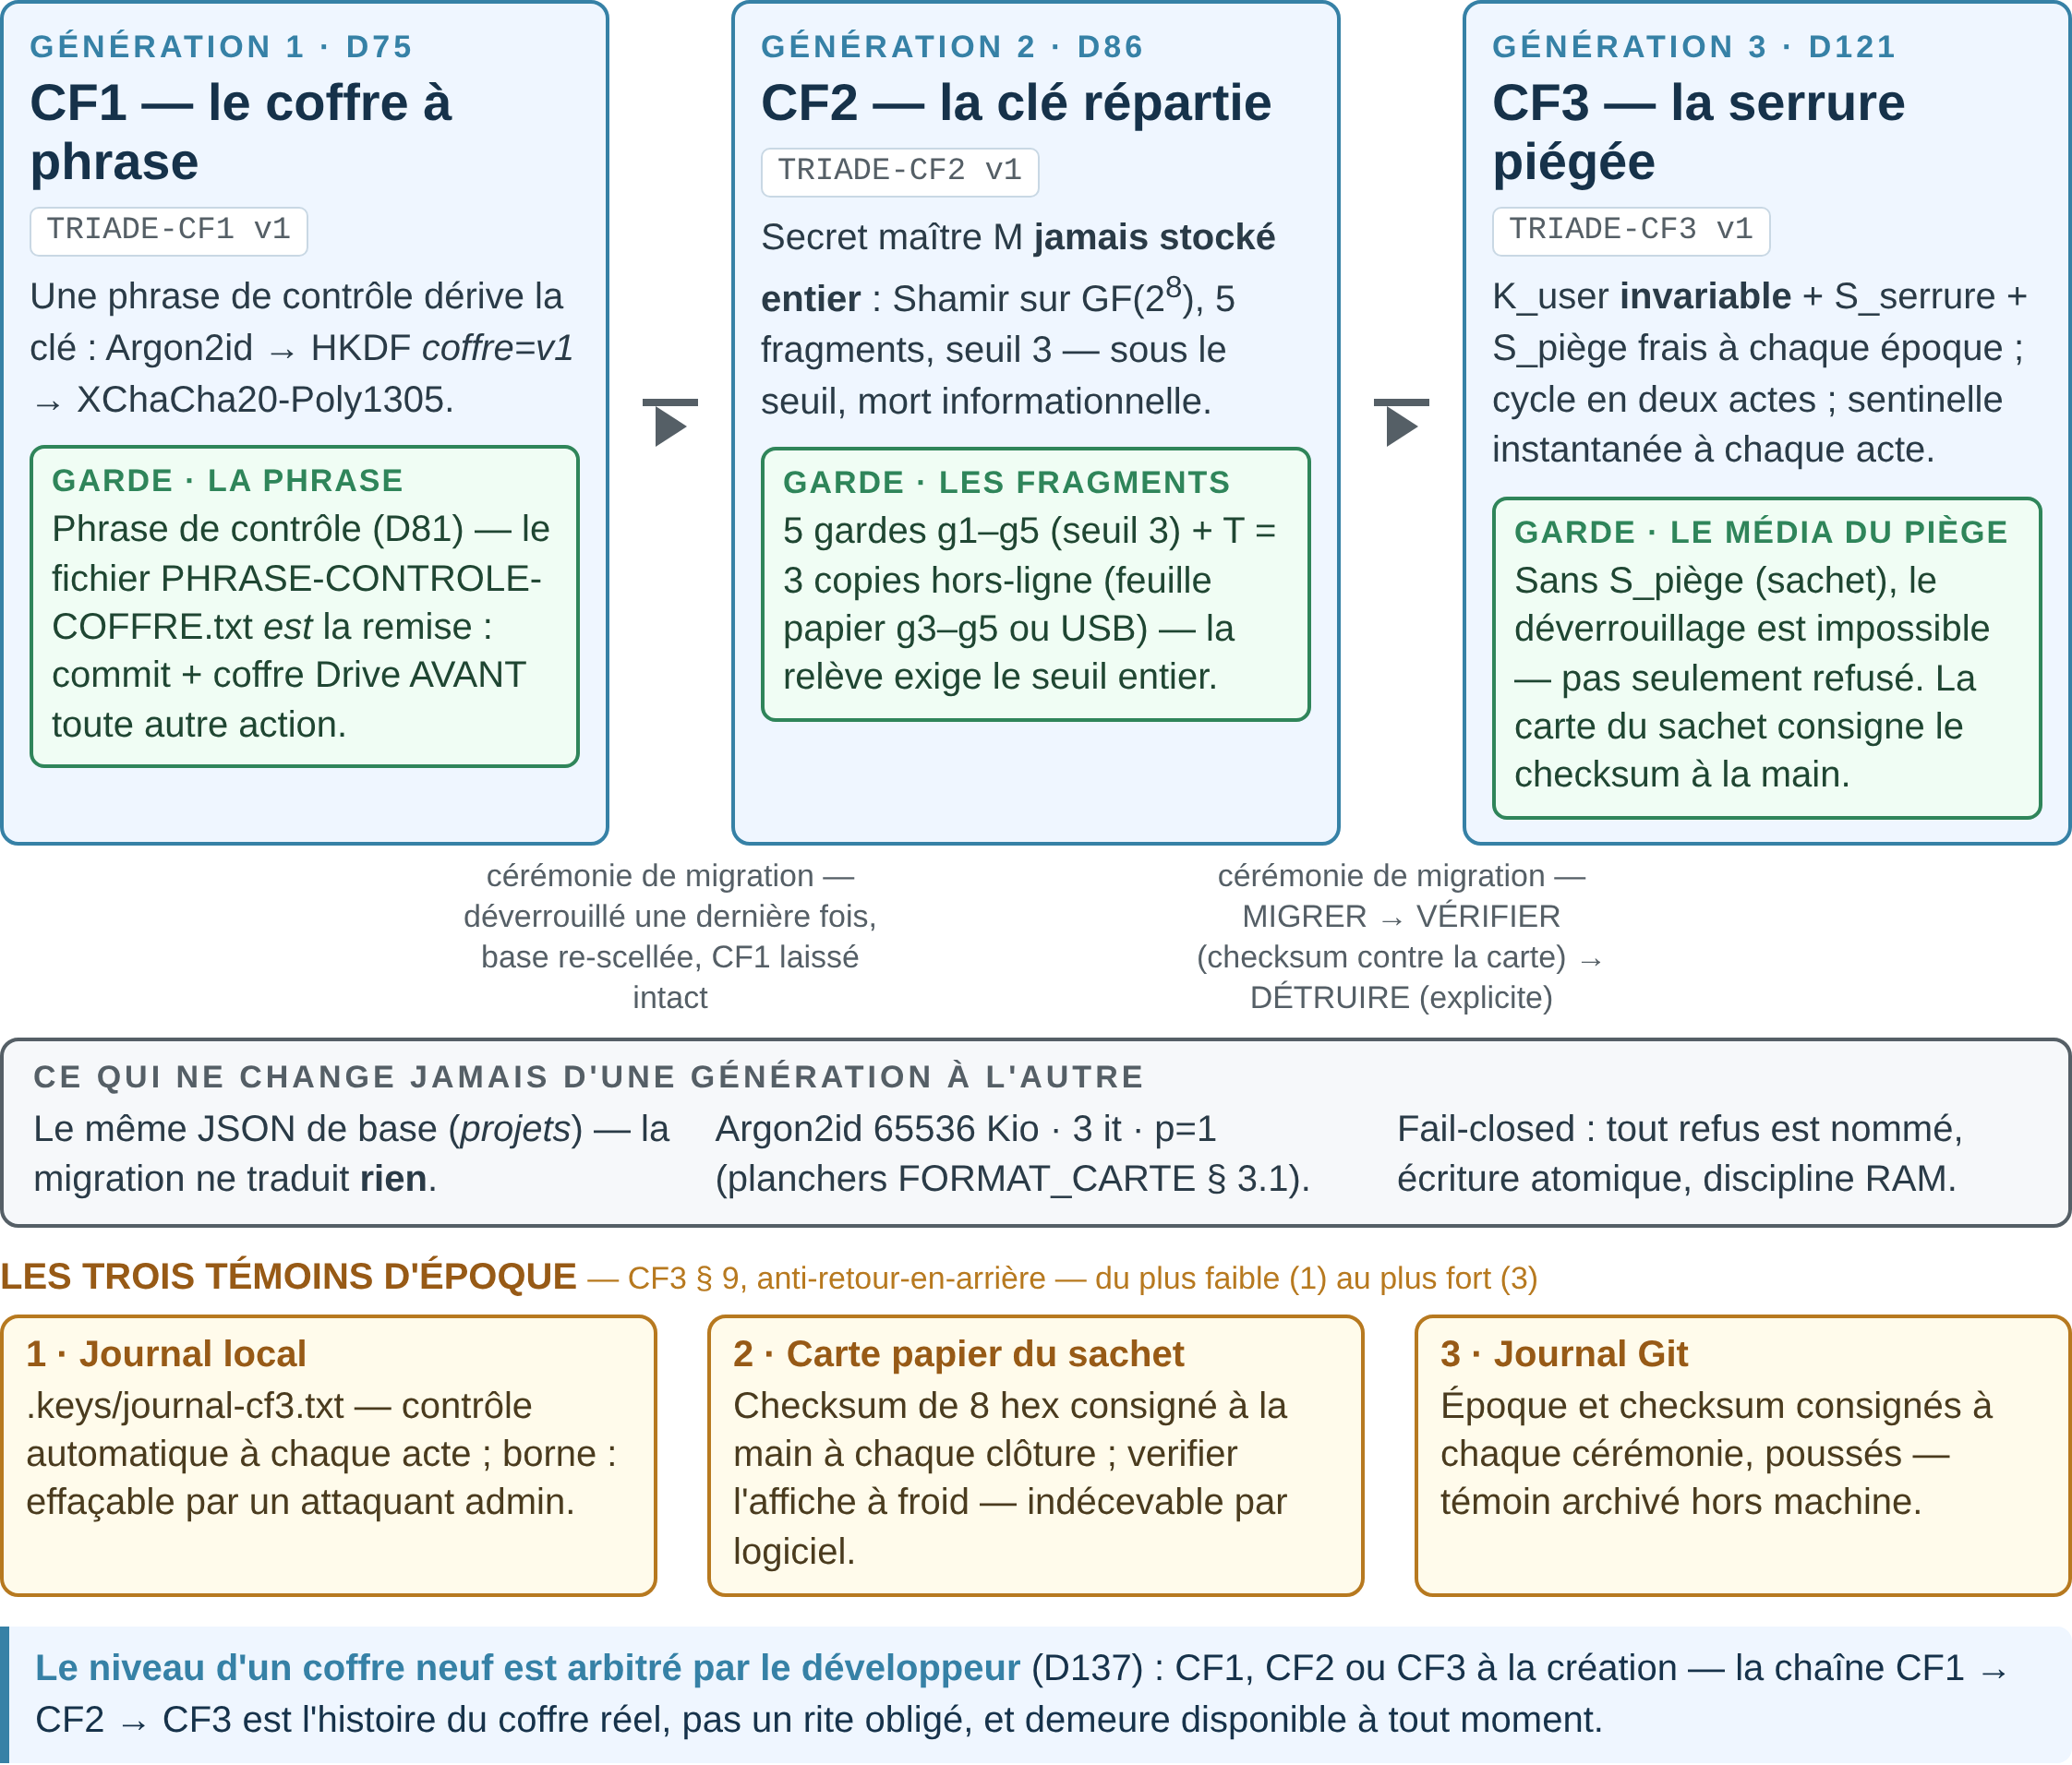
\includegraphics[width=\textwidth, max height=0.62\textheight]{chaine_cf}
\caption{La chaîne du coffre-fort : trois générations, leurs gardes, les trois témoins
d'époque. Le niveau d'un coffre neuf est arbitré par le développeur (D137) ; la chaîne
de migration est l'histoire du coffre réel — et demeure disponible à tout moment.}
\label{fig:chaine}
\end{figure}

\begin{table}[htbp]
\centering\small
\caption{Les cérémonies de la souveraineté — qui fait quoi, et la preuve attendue.}
\label{tab:ceremonies}
\begin{tabularx}{\textwidth}{@{}l Y Y@{}}
\toprule
\textbf{Cérémonie} & \textbf{Gestes} & \textbf{Preuve} \\
\midrule
Sceau de l'Intention (D87/D126) & \code{preparer} (le dépôt écrit \code{a-signer.txt}) ;
cérémonie hors-ligne \code{signer} (clé physique) ; \code{deposer} (chaque signature
vérifiée AVANT écriture) ; \code{verifier} & treize arbres VERTS, code 0 ; commit poussé \\
CF1 $\to$ CF2 (D106) & phrase de contrôle (D81 : remise AVANT tout) ; \code{migrer} ;
cinq gardes posées ; T = 3 copies hors-ligne (feuille g3--g5 ou USB) ; contrôle de
relecture ; liste blanche & CF2 \code{verifier} VERT ; CF1 laissé intact \\
CF2 $\to$ CF3 (D121/D127) & onglet MIGRER (conteneur CF2, gardes, \emph{média du piège
requis}, phrase deux fois) ; onglet VÉRIFIER (checksum contre la carte du sachet) ;
onglet DÉTRUIRE (case explicite, après recoupement) & époque 1, checksum 8 hex noté sur
la carte ; verdict à froid VERT (recommandé : re-exécution machine froide) \\
Clôture CF3 (usage courant) & acte I : ouverture, média débranché ; session sur le
brouillon ; acte II : phrase retapée, moitiés fraîches, époque N+1, re-lecture à froid
du staging & checksum affiché, ligne sur la carte du sachet ; journal Git consigné \\
Destruction locale (\code{bruler}) & commande explicite
\code{--oui-je-comprends} ; trois passes + PV & PV nommé dans \code{.keys/pv-cf3/} ;
fragments et médias \emph{jamais} touchés \\
\bottomrule
\end{tabularx}
\end{table}

\subsection{Le maître de cérémonie graphique et le trio D122}\label{sec:gui}

Les cérémonies sont conduites par le \textbf{maître de cérémonie graphique}
(\code{v06/ceremonie\_gui.py} pour le sceau et CF2 ; \code{v06/migration\_cf3\_gui.py}
pour CF2 $\to$ CF3) : zéro ligne de commande, un fichier, deux profils (repo git ou
dossier local). Le GUI est un \emph{relais} : il ne réimplémente rien — il lance
\code{coffre\_cf2.py} / \code{coffre\_cf3.py} / \code{sceau\_I.py} et croise le code de
sortie \emph{et} la marque de verdict dans le flux (un enfant menteux est rouge, un
enfant muet est sans verdict). La phrase passe par STDIN, jamais en ligne de commande,
jamais affichée, jamais dans un rapport. Chaque module à tester porte le \textbf{trio
D122} : une GUI, une boîte noire locale horodatée (gitignorée, muette si le disque
refuse — témoin, pas dépendance), un bouton « Envoyer le rapport ». L'habit a appris du
terrain : cahier numéroté comme le fil (D128), pilier droit permanent — le fil d'étapes
et le journal visibles quel que soit l'onglet (D129), un bouton d'attachement par page
(D131), disposition en grille — chaque bouton « Parcourir » sur la ligne de son champ
(D132).

\subsection{Le kit Drive — identité par construction (D130)}\label{sec:kit}

Les cérémonies s’arment depuis le dépôt \emph{ou} depuis le kit du dossier
\code{/Cérémonie} du Drive. Depuis D130, le \code{v06/} du kit est déployé depuis
\code{git ls-files v06/} — la même source que le miroir, lue dans le même arbre de
travail : \textbf{identité octet pour octet par construction}, \code{I/} et
\code{sceau-I/} inclus (preuves publiques du sceau, aucun secret). Le hook post-commit
porte le miroir \emph{puis} le kit dans le même geste — un échec kit ne bloque jamais le
miroir ni le commit, chaque retour est journalisé. Le \code{MANIFESTE.txt} du kit porte
le commit de référence et les empreintes : un kit périmé se \emph{lit}, ne se devine
pas. La racine du kit porte les lanceurs (\code{lancer\_ceremonie},
\code{lancer\_autotest\_cf3}, \code{lancer\_migration\_cf3} — \code{.bat} Windows,
\code{.sh} POSIX) aux conventions D118 : \code{v06/} d'abord, copie plate en repli,
refus nommé sans cible.

\subsection{La preuve terrain de la chaîne réelle (30--31 octobre 2026)}\label{sec:preuveterrain}

Le coffre réel du développeur a parcouru la chaîne entière, rapport de boîte noire à
l'appui : CF1 \code{statut} VERT (conteneur trouvé, en-tête TRIADE-CF1 v1, Argon2id) ;
CF1 \code{verifier} INTÈGRE ; phrase de contrôle changée pour la sienne (D110 —
re-chiffrement, nouveau sel, l'ancienne inopérante) ; un premier \code{migrer} CF2
refusé nommément (« phrase de contrôle divergente » — la remise D81 n'était pas encore
remplacée : le fail-closed a travaillé, la cérémonie a été rejouée) ; CF2 né — cinq
fragments sous \code{.keys/gardes-cf2} (seuil 3), CF1 intact, porte D120 posée en ère
sans moteur ; export de la feuille (trois fragments, gardes g3--g5, tags vérifiés avant
impression) ; puis la migration CF3 : \code{migrer} VERT (base re-scellée, schéma
identique — rien à traduire ; piège posé sur le média ; re-lecture à froide verte ;
époque 1, checksum \code{0cc89a96}, conteneur CF2 laissé intact) et \code{verifier} VERT
deux fois, checksum identique — le recoupement machine est fait. La destruction du
conteneur CF2 (acte 4) est un geste \emph{explicite} du maître, après recoupement sur
machine froide : jamais l'ancien avant le vert du neuf. Observation honnête consignée à
la passation : l'empreinte du \code{coffre\_fort.py} mesurée au clone terrain
(\code{299fd124…}) diverge de celle du dépôt (\code{8c79263b…}) — à recouper au
prochain \code{git pull} (\code{git status}) ; le fichier ne sert qu'à la migration
CF1 $\to$ CF2, déjà accomplie.

\subsection{Les cérémonies d'ère du sceau de l'Intention (5 novembre 2026)}\label{sec:ceremoniesere}

Le sceau a traversé deux cérémonies d'ère en un jour, chacune née d'un garde qui
refusait. \textbf{Ère M8} : l'ouverture du domaine \code{sys} avait étendu le
registre figé m0 et créé l'arbre m8 — le garde a nommé la dette AVANT tout build
(D162 : un diff d'intention non signé ; la clé hors-ligne du développeur requise,
le laboratoire ne signe jamais à sa place) ; le kit de cérémonie servi au dossier
\code{/Cérémonie} du Drive (la remise, le LISEZMOI pas à pas, la règle d'or
« JAMAIS generer »), la cérémonie passée sur pièces : douze arbres, les dix
inchangés rendant les MÊMES signatures que celles du 04/11 (la preuve D163 de la
réutilisation de la clé, sans jamais voir la clé privée), le garde repassé VERT
12/12 — puis le build \code{0.9.0-dev.1} né, déterministe d'un poste à l'autre.
\textbf{Ère M9} : la dette fut nommée À LA NAISSANCE (D166, règle 8) ; le geste
des 24 spécifications ayant bougé l'arbre, la charge fut RÉGÉNÉRÉE au geste de la
cérémonie (D168 : la charge de l'ouverture était périmée — une remise signée
dessus aurait laissé l'arbre divergé APRÈS installation) ; le développeur signa
hors ligne la remise de TREIZE arbres et déposa \code{signatures-I.txt} et
\code{cle-publique-I.txt} au coffre \code{/test} ; le laboratoire rapatrie,
recoupe — la clé déposée égale l'ancre \code{173fae9c…}, les ONZE arbres
inchangés rendent les signatures de l'ère M8, m0 re-signé, tls13 arbre neuf, les
empreintes vivantes égales la remise, chaque signature vérifiée Ed25519 — puis
installe canoniquement (tout vérifié AVANT toute écriture) et le garde est
repassé VERT 13/13, l'état « reelle » tenant. La règle qui en découle : la
cérémonie d'ère n'est pas une formalité de documentation — c'est le geste qui
rend le build de l'ère possible, et il suit le calendrier du garde, jamais
l'inverse. \textbf{L'ère du TGN (le domaine \code{loupe}, D171/D175)} suit la même
discipline : la dette fut nommée à la naissance de la couche I (D171, règle 8) et la
notation des 18 blocs s'accomplit sous elle — quatre chantiers, la table de routage
de loupe-09 étendue en révision nommée sans cascade — AUCUN build : la cérémonie
précède (le miroir des ères M8/M9). Le kit de cérémonie vit au dossier
\code{/Cérémonie} du Drive (la remise FRAÎCHE des quatorze arbres — la charge se
prépare AU GESTE de la cérémonie, D168 : les empreintes bougent avec chaque
révision de spécification — le LISEZMOI pas à pas, la règle d'or « JAMAIS generer »)
: le développeur signe hors ligne à la clé du 04/11 (l'ancre de toutes les ères),
ramène \code{signatures-I.txt} et \code{cle-publique-I.txt} au coffre \code{/test}
; le laboratoire rapatrie, recoupe (l'ancre de clé, les arbres inchangés rendant
les MÊMES signatures par le déterminisme Ed25519, m0 re-signé au registre étendu,
l'arbre \code{loupe} neuf), installe canoniquement — et le garde passe à QUATORZE
arbres VERTS : le build de Loupe peut naître.

\subsection{La frontière des secrets — git, \code{.keys}, sachet}\label{sec:frontiere}

La souveraineté vit de frontières \emph{lisibles} : chaque support porte ce qu'il doit
porter, jamais plus.

\begin{table}[htbp]
\centering\small
\caption{La frontière des supports — ce qui vit où, et pourquoi.}
\label{tab:frontiere}
\begin{tabularx}{\textwidth}{@{}l Y Y@{}}
\toprule
\textbf{Support} & \textbf{Ce qu'il porte} & \textbf{Ce qu'il ne porte JAMAIS} \\
\midrule
Dépôt git (poussé) & le code, la SPEC signée (\code{v06/I/}), les preuves publiques du
sceau, le journal de travail — et la \emph{phrase de contrôle} (D81 : le fichier est la
remise ; la rotation reste le remède d'une exposition) & aucun conteneur de coffre
(\code{/.keys/} gitignoré), aucun fragment, aucune graine \\
\code{.keys/} du clone & conteneurs CF1/CF2/CF3, gardes CF2 (5 fragments), config,
journaux et PV locaux, miroir d'époque & jamais dans git — le dossier entier est
gitignoré (ligne 28 du \code{.gitignore}) \\
Le sachet (média séparé) & pièges d'époque (\code{piege-CF3-epoque-N.txt}), T copies
hors-ligne des fragments, la carte papier & jamais branché pendant une session de
travail — le geste de débranchement est consigné au journal de cérémonie \\
Le Drive (miroir + kit) & le dépôt complet en miroir, le kit de cérémonie
(\code{v06/} identique au miroir par construction, D130), le conteneur CF1 de secours &
aucune graine de clé I (le dépôt ne voit que la clé publique) \\
\bottomrule
\end{tabularx}
\end{table}

L'extrait du journal de la migration réelle (boîte noire du GUI, 30/10/2026) —
l'évidence, pas la paraphrase :

\begin{lstlisting}
[CF3-migration] CF2 deverrouille une derniere fois (porte D120 honoree) :
    C:\...\triade\.keys\coffre_cf2.bin
[CF3-migration] base re-scellee sous CF3 (schema identique - rien a traduire) :
    C:\...\triade\.keys\coffre_cf3.bin (epoque 1)
[CF3-migration] piege pose sur le media : D:/piege-CF3-epoque-1.txt
[CF3-migration] re-lecture a froid du scellage : VERTE
[CF3-migration] VERDICT : VERT - epoque 1, checksum 0cc89a96 (1 projet(s))
    - notez-le sur la carte du sachet (spec  9)
[CF3-migration] conteneur CF2 laisse INTACT : C:\...\triade\.keys\coffre_cf2.bin
--- VERDICT migration (actes 1-3) : VERT (code de sortie 0,
    marque « VERDICT : VERT » vue dans le flux)
\end{lstlisting}

\subsection{Référence des commandes}\label{sec:commandes}

Les vérités vivantes que les GUI relaient — la CLI reste la référence (le GUI ne
réimplémente rien) :

\begin{table}[htbp]
\centering\small
\caption{Les commandes du coffre et du sceau (CLI de référence).}
\label{tab:commandes}
\begin{tabularx}{\textwidth}{@{}l >{\raggedright\arraybackslash}p{4.3cm} Y@{}}
\toprule
\textbf{Outil} & \textbf{Commande} & \textbf{Rôle} \\
\midrule
\code{coffre\_cf3.py} & \code{init} & coffre neuf : époque 1, sel et moitiés posés,
piège Nº 1 sur le média \\
 & \code{ouvrir} & acte I : sentinelle + verdict, brouillon sous K\_session \\
 & \code{verifier} & verdict à froid (sentinelle complète, aucune écriture) —
l'outil du recoupement humain \\
 & \code{statut} & étiquette seule — aucune clé dérivée, aucune phrase exigée \\
 & \code{fermer} & acte II : moitiés fraîches, époque N+1, re-lecture à froid du
staging, remplacement atomique \\
 & \code{bruler} & destruction locale MANUELLE (\code{--oui-je-comprends}) — trois
passes + PV \\
 & \code{migrer} & cérémonie CF2 $\to$ CF3 : actes 1--3, CF2 laissé intact \\
 & \code{detruire-cf2} & acte 4 : destruction EXPLICITE du conteneur CF2 (garde
fail-closed si CF3 absent) \\
 & \code{autotest} & autocontrôles sur répertoires temporaires — aucun coffre réel
touché \\
\code{coffre\_cf2.py} & \code{init · migrer · verifier · statut · lister} ; \code{obtenir · ajouter ·
retirer · restaurer · bruler} ; \code{etat-fragments · autotest} & le miroir CF1 de
ces gestes, sur la clé répartie — le détail vit dans la spec scellée CF2 § 8 \\
\code{sceau\_I.py} & \code{preparer · deposer · signer-test · verifier · etat} &
l'intention : prépare la charge à signer, dépose une remise vérifiée, garde le dépôt
(codes 0/10/11/12) \\
\code{ceremonie\_hors\_ligne.py} & \code{generer · signer · verifier} & la cérémonie
air-gap (stdlib seule) : graine, signatures, audit autonome \\
\bottomrule
\end{tabularx}
\end{table}

\paragraph{Cycle de vie d'un coffre neuf.} \code{init} (époque 1, média du piège
désigné dès le premier jour) ; usage courant en cycles \code{ouvrir} /
\code{fermer} — chaque clôture ajoute une ligne à la carte du sachet et incrémente
l'époque ; \code{verifier} à froid après toute doute (recommandé : machine froide le
lendemain d'une cérémonie) ; \code{bruler} le jour où le coffre doit mourir — jamais
avant d'avoir constitué la relève (sachet complet). Les cérémonies de migration
(\code{migrer} CF1 $\to$ CF2 puis CF2 $\to$ CF3, \code{detruire-cf2} en acte explicite)
sont l'histoire d'un coffre né avant sa génération de serrure — un coffre né CF3 ne les
connaît jamais.
  % 12 Souveraineté cryptographique · 13 Cérémonies et kit du terrain
% =====================================================================
%  CH 12-16 : Gouvernance · Menaces et limites · Jalons · Correspondance · Décisions
% =====================================================================
\section{Gouvernance}\label{sec:gouvernance}

\subsection{Journal des décisions — format normalisé}\label{sec:journal}

Le protocole ne se révisant jamais en silence, chaque décision structurante est consignée
dans un journal. La v0.4.0 normalise le format (D24) :

\begin{table}[htbp]
\centering\small
\caption{Format normalisé d'une entrée du journal des décisions.}
\label{tab:formatdecisions}
\begin{tabularx}{\textwidth}{@{}l Y@{}}
\toprule
\textbf{Champ} & \textbf{Exigence} \\
\midrule
ID & \code{DNNN}, séquentiel, jamais réutilisé \\
Date & date de consignation \\
Statut & active · amendée par Dxx · invalidée par Dxx \\
Contexte & exigence, incident ou évaluation qui motive la décision \\
Choix retenu & décision en une phrase, rattachée à la fonction objectif \\
Alternatives rejetées & au moins une, avec motif \\
Amendements & référence explicite à la décision remplacée, le cas échéant \\
Développement & argumentaire détaillé si la décision engage l'architecture \\
\bottomrule
\end{tabularx}
\end{table}

Trois règles : le journal est \textbf{append-only} (une entrée ne s'efface jamais) ; une
révision \textbf{invalide explicitement} ce qu'elle remplace ; aucune entrée n'est
rétrodatée. La conformité du journal — présence des champs, unicité des ID, chaînage des
amendements — est contrôlée mécaniquement par l'audit de gouvernance.

\subsection{Tableau de bord de conformité}\label{sec:tableaudebord}

La v0.4.0 unifie les indicateurs de santé en un \textbf{tableau de bord} (D24), généré par
la commande d'audit à chaque commit et à chaque cristallisation, archivé avec la carte :

\begin{table}[htbp]
\centering\small
\caption{Tableau de bord de conformité : métriques, cibles, sources.}
\label{tab:dashboard}
\begin{tabularx}{\textwidth}{@{}Y l Y@{}}
\toprule
\textbf{Métrique} & \textbf{Cible} & \textbf{Source de mesure} \\
\midrule
Blocs avec spécification I à jour & 100 \% & audit de traçabilité \\
Chaînes de traçabilité complètes I $\leftrightarrow$ C $\leftrightarrow$ B
$\leftrightarrow$ tests & 100 \% & audit de traçabilité \\
Construction & 0 / 0 & build \\
Tests différentiels & 100 \% verts & oracle \\
Empreintes des données embarquées & conformes & hachage vs carte \\
Défauts ouverts par classe T1–T6 & 0 & journal des décisions \\
Optimisations sans mesure (R11) & 0 & journal d'optimisation \\
Budgets tokens (localiser / éditer / ajouter) & $\leq$ 64 / 3 000 / 6 000 &
instrumentation — mesurés M1 : 51 / 719 / 1 088 (D31) \\
Suite de conformité par profil actif & verte & suite du profil \\
Changements hors journal des décisions & 0 & diff vs journal \\
Pré-versions correctement balisées (dev / rc / final) & 100 \% & registre des balises \\
\bottomrule
\end{tabularx}
\end{table}

Le tableau de bord est la contrepartie mesurable de la gouvernance : chaque affirmation du
protocole s'y retrouve sous forme de métrique avec sa cible et sa source — aucune ne
s'appuie sur une déclaration non vérifiable. Les métriques dépendantes de l'outillage
affichent leur statut « cible » jusqu'à leur premier mesurage.

\subsection{Continuité et anti-enfermement}

L'export de continuité (D16) demeure l'unique forme de transfert de l'état de
développement : conteneur chiffré et signé regroupant I, B, C et un manifeste
autodescriptif ; oracle régénéré depuis I à l'arrivée, jamais exporté ; import en cinq
étapes dont l'échec d'une seule est terminal. Sauvegarde 3-2-1 chiffrée et escrow de la
clé maîtresse inchangés.

\paragraph{Le coffre-fort des phrases maîtresses (D75).} Le composant qui centralise
toutes les phrases maîtresses d'un projet — et de tout projet ultérieur conduit sous le
protocole — dans un conteneur unique chiffré TRIADE-CF1 (\code{coffre\_fort.py}) :
phrase de contrôle sous garde durable (D81 — sauvegardée dès production au dépôt et au
racine du coffre Drive, AVANT toute autre action), Argon2id aux
planchers de la carte au repos puis HKDF à contexte dédié, XChaCha20-Poly1305 avec
l'en-tête clair pour AAD, écriture atomique 0600, autotest de falsification exigé à
chaque installation. Le conteneur chiffré s'exporte tel quel vers le coffre Drive du
projet et le coffre personnel du développeur — son vol relève de la menace « vol du
coffre-fort des phrases », étendue en D81. Après une réinitialisation du poste, l'import
du conteneur, la relecture de la phrase depuis \code{PHRASE-CONTROLE-COFFRE.txt}, puis
\code{obtenir --vers-fichier} restaurent la phrase opérationnelle sans cérémonie
de régénération. Discipline évoluant en D81 sur un point, l'arbitrage (risque de PERTE
vécu contre risque d'EXPOSITION théorique) étant consigné : chaque cérémonie de clés
(D27/D30) alimente le coffre dans la même session, la phrase de contrôle est sauvegardée
durablement AVANT TOUTE AUTRE ACTION — \code{PHRASE-CONTROLE-COFFRE.txt} au racine du
dépôt (commit dédié, push GitHub, miroir Drive par le hook) et au racine du coffre
Drive, md5 vérifiés : le fichier est la remise, l'affichage unique cesse d'être le canal
de survie — et la graine Ed25519 reste hors coffre (D30). Contrepartie consignée : la
phrase vit sur le stockage du coffre Drive partagé par lien — la confidentialité au
repos repose sur le contrôle d'accès au dossier (restreindre le partage par lien :
mitigation première) ; une phrase entrée dans l'historique git y demeure à vie, la
rotation reste le remède — format normatif : FORMAT\_CARTE § 11.

\section{Menaces et limites}\label{sec:menaces}

Le principe directeur demeure : séparer l'obfuscation, qui protège la propriété
intellectuelle, du durcissement, qui protège l'exécution. Conformément au principe de
Kerckhoffs, la sécurité ne repose jamais sur le secret de la carte : elle survivrait à sa
divulgation.

\subsection{Modèle de menace (étendu en v0.4.0, D20)}

\begin{table}[htbp]
\centering\small
\caption{Modèle de menace — ajouts v0.4.0 en gras ; ajout v0.5.1 en gras (D75), étendu v0.5.2 (D81) ; ajouts v0.6.0 en gras (D84--D87, D121, D133).}
\label{tab:menaces}
\begin{tabularx}{\textwidth}{@{}Y Y Y@{}}
\toprule
\textbf{Menace} & \textbf{Contre-mesure} & \textbf{Résiduel} \\
\midrule
Rétro-ingénierie de l'IP & carte privée ; binaire sémantiquement muet ; variantes par
build & temps acheté — s'érode avec les LLM de décompilation \\
Empoisonnement de carte & signature ; refus de carte non signée ; verrou croisé (R8, R9)
& détecté — session bloquée \\
Corruption de carte (accidentelle) & AEAD par fragment + signature + verrou & détecté au
chargement \\
Fuite de la carte & chiffrement ; sharding ; escrow & perte limitée à un fragment \\
Vol de l'export de continuité & chiffrement intégral + signature & indéchiffrable sans
la phrase \\
\textbf{Vol du coffre-fort des phrases} & chiffrement intégral (Argon2id, contexte
HKDF dédié, AEAD) ; écriture atomique ; depuis D81 la phrase de contrôle vit au coffre
Drive et au dépôt — mitigation première : restreindre le partage par lien & confidentialité
ramenée au contrôle d'accès du dossier ; une phrase commise en git y demeure à vie — la
rotation reste le remède (D75, étendu D81) \\
\textbf{Expropriation (employeur, tiers)} & barrière juridique BSL 1.1 (D84) ;
barrière cryptographique : clé maîtresse jamais entière (Shamir, axe 2), intention
signée par la clé hors-ligne (sceau I, axe 3), serrure piégée à média séparé (axe 4) &
le code volé est inexploitable et ne peut pas évoluer ; l'axe 1 (TEE) reste une
exigence consignée \\
\textbf{Binaire altéré} & checksums par bloc + signature du manifeste au lancement
(R10 a, b) & détecté — arrêt avant tout effet \\
\textbf{Rollback non autorisé} & monotonie de version signée, plancher anti-rollback
(R10 c) & détecté — refus \\
\textbf{Evil maid sur le conteneur ou le média du piège} & tag du piège, époques
croisées conteneur/piège, AEAD + étiquette, champ \code{verif} indérivable (CF3
§ 5) & détecté — refus nommé ; la falsification prouvée détruit côté machine,
jamais le média \\
\textbf{Roll-back du couple conteneur + piège} & trois témoins d'époque : journal
local, carte papier du sachet (à la main), journal Git poussé (CF3 § 9) & détecté —
« RETOUR EN ARRIÈRE » nommé ; recoupement humain à froid \\
\textbf{Agent défaillant} & R2 ; R5 ; oracle dérivé de I ; budgets & l'erreur ne devient
jamais permanente sans vérification \\
\textbf{Données embarquées modifiées} & empreintes dans la carte ; vérification au
lancement (R10 b) & détecté — arrêt propre \\
\textbf{Environnement non conforme} & contrôles de conformité au profil (R10 d) ;
fail-closed & refus propre avant exécution \\
Fuzzing boîte noire & contrats, oracle, tests par propriétés & indépendant du secret de
la carte \\
Redistribution frauduleuse & empreintes par build — canary trap & fuite traçable \\
Instrumentation dynamique & anti-debug léger par mesure de temps & assumé \\
\bottomrule
\end{tabularx}
\end{table}

Les six menaces en gras sont les additions de la v0.4.0, le vol du coffre-fort (D75)
celle de la v0.5.1 ; toutes sont neutralisées par des mécanismes \textbf{locaux et
vérifiables} — la contre-mesure anti-rollback ne dépend d'aucun service en ligne (le
chargement doit échouer proprement hors ligne), et les vérifications de R10 s'exécutent
avant toute entrée dans le chemin d'exécution.

\subsection{Limites assumées}\label{sec:limites}

La rétro-ingénierie est un objectif d'économie, pas d'impossibilité : le coût de l'analyse
d'un binaire strippé, sans structure, dont chaque exemplaire diffère, reste supérieur à sa
valeur — mais les modèles de langage appliqués à la décompilation progressent, et
l'avantage doit être réévalué à chaque génération. L'anti-debug reste léger et assumé.
La furtivité face aux EDR est hors périmètre : un outil légitime par construction, dont
la transparence vis-à-vis du système est totale. Enfin, la gouvernance du protocole a été
validée sur un cas unique (N = 1) — l'étude de cas RoomEq, dont les limites sont
documentées dans l'édition académique (D18) : la généralité reste à établir par
réplication, le cœur natif par les jalons M0 à M7.

\section{Critères d'acceptation des jalons M0 à M10}\label{sec:jalons}

Onze jalons, chacun avec des critères de sortie mesurables (détail dans
\code{PLAN\_MILESTONES.md}). \textbf{Conditions transverses} (v0.4.0) : aucun jalon n'est
franchi sans oracle vert, suite de conformité verte pour les éléments couverts, tableau de
bord conforme et carte signée.

\begin{table}[htbp]
\centering\small
\caption{Critères d'acceptation des jalons.}
\label{tab:jalons}
\begin{tabularx}{\textwidth}{@{}l Y >{\raggedright\arraybackslash}p{2.6cm}@{}}
\toprule
\textbf{Jalon} & \textbf{Critères de sortie mesurables} & \textbf{Statut} \\
\midrule
M0 — chaîne artefact & exécution sur Windows 11 ; round-trip 100 \% ; carte v0 signée ;
exécutable $<$ 4 Kio ; R1–R3, R8–R9 dès le premier octet & \textbf{franchi} 26/10/2026 (D26) \\
M1 — blocs réutilisables & oracle 100 \% sur la mini-libc ; première cristallisation ;
adresses stables démontrées ; première mesure effective des budgets tokens & \textbf{franchi} 26/10/2026, 0.2.0 (D32) \\
M2 — patch à chaud & remplacement du bloc d'écho en exécution, sans interruption ;
rollback démontré ; régression post-patch nulle & \textbf{franchi} 27/10/2026, 0.3.0 (D43) \\
M3 — entrées non fiables & un million de requêtes fuzzées sans crash ; proxy
transparent ; contrats renforcés & \textbf{franchi} 28/10/2026, 0.4.0 (D74) \\
M4 — tunnel chiffré & HTTPS en transit ; échec propre sur certificat invalide & \textbf{franchi} 29/10/2026, 0.5.0 (D99 — tunnel chiffré établi et certificat rejeté sur machine réelle, terrain.17-D ; balise scellée, arbre \code{m4/I} signé) \\
M5 — outil complet & interception d'un flux navigateur en VM isolée ; patch à chaud du
journal en production ; empreintes par build actives ; programme d'étapes et critères
dans \code{PLAN\_MILESTONES.md} & \textbf{franchi} 04/11/2026, \code{0.6.0} (Entrée 143, D148 : critère (b) de D136 vert sur pièces au run e4 ; le chantier (c) refermé au M6 sur le profil Linux) \\
M6 — portabilité inter-OS & suite de conformité verte ; \textbf{diff nul sur la couche
I} ; parité inter-profils vérifiée ; même oracle vert sur les deux profils & \textbf{franchi} 05/11/2026, \code{0.7.0} (Entrée 149, D154 : run terrain WSL2 vert sur pièces, recoup labo 22/22 — le noyau de la machine du développeur distinct de celui du labo) \\
M7 — portabilité inter-ISA & round-trip 100 \% sur la nouvelle ISA ; suite de conformité
verte ; patch à chaud conforme (scratch + \code{fence.i}) ; verrou multi-profils ; export
multi-profils vérifié & \textbf{franchi} 05/11/2026, \code{0.8.0} (Entrée 155 : run terrain M7-(d) vert sur pièces, recoup labo 29/29, export multi-profils de bout en bout — l'universalité démontrée : win \code{0.6.0} / linux \code{0.7.0} / riscv \code{0.8.0}) \\
M8 — syscalls directs (domaine \code{sys}) & la charte à huit règles et les spécifications sys-01…03 écrites-avant-code ; le harnais sur fixtures \code{ntdll} synthétiques (le labo ne connaît jamais le SSN du terrain) ; le motif du stub vérifié avant toute extraction ; le run terrain sur le VRAI \code{ntdll} — la même observable par les DEUX chemins ; la cérémonie de l'ère avant le build & \textbf{franchi} 05/11/2026, \code{0.9.0} (Entrées 156--164, D160--D165 : harnais 61 verts ; cérémonie de l'ère passée 12/12 ; run terrain m8d vert — 35 verts / 0 échec, la twin octet pour octet, le refus $-4$ du stub crocheté ; recoup labo 30/30 ; finale scellée sur recoup exigé comme pièce) \\
M9 — TLS 1.3 pur (domaine \code{tls13}) & la charte à huit règles et les 28 spécifications en six familles écrites-avant-code ; les primitives aux vecteurs officiels (FIPS 180-4, RFC 2104/4231, RFC 5869, RFC 7748, SP 800-38D) ; la poignée rejouée sur le transcript RFC 8448 ; le socle socket par syscalls directs (sys-04+) ; la cérémonie de l'ère avant \code{construire()} ; la session réelle — la ligne applicative chiffrée & \textbf{franchi} 07/11/2026, \code{1.0.0} (Entrées 170--194, D166--D170 : les 28 blocs notés-mesurés-prouvés aux vecteurs officiels, la poignée sur le transcript RFC 8448, le socle socket par syscalls directs ; le septième run terrain vert recoupé 34/34 sur pièces croisées, LA SESSION RÉELLE — la ligne applicative chiffrée échangée avec un serveur réel, le témoin « HTTP/1.1 200 OK » déchiffré par la machine, l'épinglage $-6$ nommé ; la finale scellée sur recoup exigé comme pièce, \code{proxy.exe} byte-identique \code{446279f3…}) \\
M10 — le test grandeur nature « Loupe » (domaine \code{loupe}) & coder une application réelle NEUVE entièrement avec TRIADE, de l'intention (la couche I) à l'octet livré (le kit terrain) ; les 18 spécifications écrites-avant-code avant tout octet de notation (R2) ; les héritages PAR LA CARTE byte-identiques aux adresses scellées (R7) ; l'oracle à scénarios vert — l'écran attendu octet par octet ; le kit déployé au coffre \code{/test} (modèle m9f) ; la balise \code{loupe 0.1.0} scellée sur run terrain recoupé & \textbf{ouvert} 07/11/2026 (D171) — la couche I complète (18 spécifications, D172) et les QUATRE chantiers de notation accomplis : le noyau (D173), le rendu + la navigation (D174), l'édition + la table de routage étendue de loupe-09 r2 (D175) — les 18 blocs NOTÉS-MESURÉS-PROUVÉS (59 + 53 + 45 contrôles verts aux trois graines) ; LA CÉRÉMONIE D'ÈRE du TGN PASSÉE SUR PIÈCES (le 14e arbre, la dette D166/D171 SOLDÉE — le garde 14/14) ; le kit terrain livré (M10-(d)) ; LE RUN (M10-(e)) REFUSÉ TROIS FOIS, CHAQUE REFUS NOMMÉ : dev.1 puis dev.2 du refus du chargeur 0xc000007b (l'oubli du BASERELOC, puis la table nécessaire mais PAS suffisante), puis LE PAS DÉCISIF — LE VRAI CHARGEUR A CARTOGRAPHIÉ dev.3 (l'enveloppe PROUVÉE au terrain) et LE TÉMOIN A NOMMÉ AU T0 [CADRE-NÉ] (l'initialiseur du build : le sentinel à +8, une TAILLE prise pour un offset, au lieu de +528 la chaîne des tailles) ; LA RETOUCHE dev.4 DÉPOSÉE : l'initialiseur \code{.data} MIROIR EXACT du \code{CADRE\_VIERGE} du harnais, LE GARDE GUÉRI (le validateur relit LE MÊME miroir — le contrôle dérive du plan, jamais de la pièce qu'il contrôle), ET le scénario relit LE \code{.data} ENTIER contre le miroir ; LE QUATRIÈME RUN EST LE PAS LE PLUS LOIN JAMAIS VÊCU : [T0] TOUT VERT (l'image cartographiée, LE CADRE NÉ MIROIR — la retouche TENUE au terrain, l'IAT 37 feuilles posées) PUIS [T1] ÉCHEC NOMMÉ [SESSION] : loupe-01 a rendu $-6$ SYSTÈME, le fichier pourtant relu à l'instant — ET LA VITRINE A VÉCU SA PREMIÈRE FOIS (« la fenêtre s'ouvre et se referme immédiatement » : la mort SANS TÉMOIN) ; L'AUTOPSIE NOMME LA CLASSE DES ARGUMENTS PILE (les 5+ de l'ABI msx64 AU HOME SPACE au lieu de \code{[rsp+0x20]+} : loupe-01/05/06 — le VRAI ReadFile lisait le contexte condensé COMME UN POINTEUR), L'AUDIT D'ABI msx64 NÉ AU BUILD nomme DEUX AXES D'ALIGNEMENT (loupe-10 le sous-programme \code{.peindre} pile $\equiv 8$ — le VRAI gdi32 SSE ; loupe-11 le cadre \code{0x38}), LE GARDE GUÉRI PAR LA CONVENTION (les shims relisent LES MÊMES SLOTS QUE LE VRAI — V7 : la falsification demandée, attrapée), ET LE KIT PORTE SON TÉMOIN VITRINE (\code{temoin-vitrine.bat} — la prochaine mort sera nommée) ; LA RETOUCHE dev.5 DÉPOSÉE : \code{loupe.exe 0.1.0-dev.5} (127 488 o, sha256 \code{6f830f9c…}), 159 contrôles verts (61+53+45 — V7 NÉ) ; LE CINQUIÈME RUN A NOMMÉ $-7$ VERROUILLÉ — ET LA PIÈCE ACQUITTÉE (l'Entrée 208) : l'appel CreateFileW était NÉ PARFAIT (la classe de l'Entrée 207 TENUE, LA PREUVE PAR LE NOM CHANGÉ : $-6$ devint $-7$ — un refus NÉ, refusé pour une RAISON RÉELLE), C'ÉTAIT LE KIT QUI FAUTAIT (le scénario EST LE CHARGEUR : l'image TIENT loupe.exe, le VRAI Windows refuse gle 32 l'écriture sur une section vivante — T1 offrait la pièce à l'écriture, IMPOSSIBLE PAR CONSTRUCTION), loupe-01 a traduit le refus AU NOM PRÈS — LA VOIE NOMMÉE A VÉCU SON PREMIER TERRAIN ; LA RETOUCHE dev.6 AU KIT SEUL (l'artefact INCHANGÉ) : L'OMBRE \code{temoin-session.bin} (la copie byte-à-byte née et morte au run), LE FRÈRE DE T6 CHASSÉ (la session double offre l'ombre, jamais la pièce), LA VITRINE SE VIT PAR SON TÉMOIN (\code{temoin-vitrine.txt} REQUIS), le run rejoué attend le développeur \\
\bottomrule
\end{tabularx}
\end{table}

M0 est le jalon existentiel — il prouve la chaîne notation, octets, exécutable, exécution
sans compilateur. M2 est le jalon de vérité — le patch à chaud a motivé l'architecture.
M6 et M7 transforment la portabilité de promesse en propriété démontrée, en isolant chaque
variable ; la suite de conformité par profil en est désormais le critère d'acceptation
explicite. M8 et M9 sont les additions mesurées du programme d'après M7 (D160) : la
fondation d'abord — le domaine \code{sys} est la condition d'une pile TLS 1.3 qui
n'émettrait plus par l'IAT userland ; chaque famille s'appuie sur les résultats
mesurés de la précédente. M10 est l'épreuve de la MÉTHODE ENTIÈRE (D171) : non plus
une capacité, mais une application réelle neuve — l'outil du quotidien du projet —
développée de l'intention à l'octet livré, chaque geste prouvé ; la notation entière
(18 blocs) est notée-mesurée-prouvée, la cérémonie d'ère est PASSÉE (le garde à
quatorze arbres), le build est NÉ — et LE TERRAIN répond : trois refus NOMMÉS,
deux du chargeur (0xc000007b — l'oubli du BASERELOC, puis la table nécessaire
mais pas suffisante), puis LE PAS DÉCISIF : l'image cartographiée par LE VRAI
chargeur (l'enveloppe prouvée DEMEURE) et l'échec [CADRE-NÉ] nommé AU TÉMOIN
par le T0 du scénario — la retouche dev.4 fait de l'initialiseur \code{.data} LE
MIROIR EXACT de l'état de naissance prouvé par le harnais, et le garde du build
relit LE MÊME miroir : le contrôle dérive du plan, jamais de la pièce qu'il
contrôle.

\paragraph{Le programme d'après M7 (D160).} La clôture v0.6.1 tenait les additions
mesurées « hors périmètre courant » ; la v0.7.0 lève la clause pour les deux
premières familles, sur résultats mesurés. \emph{M8, les syscalls directs} (domaine
\code{sys}) : la charte à huit règles — le SSN est une donnée, jamais un octet de
code ; le motif du stub est vérifié avant toute extraction ; un stub divergent est
un refus nommé — et la preuve d'observable : la MÊME ligne émise par les deux
chemins (l'IAT \code{kernel32} de hello-02 et le syscall direct \code{NtWriteFile}
de sys-03), comparées octet pour octet au fixture. \emph{M9, TLS 1.3 pur} (domaine
\code{tls13}, ère 1.0.0) : la grande œuvre de la souveraineté complète — la
cryptographie de session sans délégation, la couche I complète (28 spécifications,
six familles), la cérémonie d'ère passée (13 arbres, garde 13/13). L'ordre est la
fondation d'abord : une pile TLS pure qui émettrait encore par l'IAT userland
garderait la surface de hook qu'elle prétend éliminer.

\paragraph{Le test grandeur nature (D171).} Le protocole a prouvé chaque capacité,
M0 à M9 ; il reste à prouver qu'il DÉVELOPPE une application réelle NEUVE, de
l'intention à l'octet livré — le modèle RoomEq (v0.3) s'arrêtait au recodage d'une
application existante, le TGN exige la CRÉATION. L'application arbitrée est
« Loupe », l'éditeur hexadécimal natif au panneau d'empreintes sur le profil
primaire (\code{loupe.exe}, la lignée de balises propre \code{loupe 0.1.0-dev.1} au
premier build) : voir les octets, leurs lignes, leurs empreintes md5/sha-256, leur
place — l'outil du quotidien du projet. La découpe du plan est la loi : la cérémonie
d'ère précède le build (le miroir M8/M9 — Entrées 157/158), la notation s'accomplit
sous la dette nommée (D166/D171).

\paragraph{Archivé (D133, pour mémoire).} Le jalon de l'outil complet s'ouvrit sur trois
chantiers mesurables : (a) \emph{empreintes par build actives} — chaque build consigne
l'empreinte de son artefact dans le tableau de bord et le journal de travail, la
comparaison inter-build devient un contrôle automatique ; (b) \emph{interception d'un
flux navigateur en VM isolée} — le proxy transparent M3 porte le tunnel M4 au scénario
réel complet ; (c) \emph{patch à chaud du journal en production} — l'écriture vivante
du superviseur terrain sous patch, le retour arrière prêt. L'ordre est dicté par la
dépendance : (a) arme la preuve dont (b) et (c) ont besoin pour être auditables.

\section{Correspondance des versions}\label{sec:correspondance}

\subsection{Traçabilité des évolutions}\label{sec:evolutions}

\begin{table}[htbp]
\centering\small
\caption{Les dix-sept évolutions de la v0.4.0, tracées depuis la v0.3.}
\label{tab:correspondance}
\begin{tabularx}{\textwidth}{@{}l Y Y l@{}}
\toprule
\textbf{Évolution} & \textbf{En v0.3} & \textbf{En v0.4.0} & \textbf{Statut} \\
\midrule
Couche I normalisée & « contrats légers » sans gabarit & gabarit complet
(§\ref{sec:coucheI}) & renforcé (D19) \\
Taxonomie des défauts & absente & classes T1–T6 (§\ref{sec:taxonomie}) & nouveau (D19) \\
Threat model & 7 menaces & 13, dont 6 nouvelles & étendu (D20) \\
R10 & checksums au lancement & + signature, anti-rollback, conformité, fail-closed
explicite & renforcé (D20) \\
Optimisation prématurée & interdite implicitement & interdiction normative R11 &
explicité (D21) \\
Journal d'optimisation & pratique de démonstration & format OPT-NN & officialisé (D21) \\
Fragmentation & 4 fragments & + norme « aucune lecture totale » & consolidé (D24) \\
Localisation par intention & étape 2 implicite & balayage interdit, formalisé &
renforcé (D24) \\
Budgets tokens & 64 / 3 000 / 6 000 & localiser amendé après mesure M1, instrumentés & consolidé (D24, D31) \\
Suite de conformité profil & implicite & suite obligatoire (§\ref{sec:conformite}) &
nouveau (D22) \\
Parité inter-profils & critères dispersés & définition formelle (§\ref{sec:parite}) &
formalisé (D22) \\
Reverse-specs & absente (pratique démo) & officialisées (§\ref{sec:reversespecs}) &
officialisé (D23) \\
Pré-versions & absente (pratique \code{-dev.1}) & dev / rc / final & officialisé (D23) \\
Fixtures partagées & absente (pratique installateur) & contractuelles & officialisé
(D23) \\
Traçabilité I–C–B–tests & implicite & table normative + audit & formalisé (D24) \\
Journal des décisions & pratique & format normalisé & normalisé (D24) \\
Tableau de bord & indicateurs dispersés & métriques unifiées & nouveau (D24) \\
\bottomrule
\end{tabularx}
\end{table}

\subsection{Modifications explicitement rejetées}\label{sec:rejets}

Conformément au cahier de révision, les modifications suivantes ont été examinées et
\textbf{rejetées, donc non appliquées} :

\begin{table}[htbp]
\centering\small
\caption{Modifications examinées et rejetées.}
\label{tab:rejets}
\begin{tabularx}{\textwidth}{@{}Y Y@{}}
\toprule
\textbf{Modification} & \textbf{Motif du rejet} \\
\midrule
Modifier la hiérarchie Sécurité $>$ Performance $>$ Optimisation $>$ Coût en tokens &
invariant de révision (D19) — condition même de l'arbitrage \\
Introduire une couche d'abstraction à l'exécution (bytecode, VM) & trahit la fonction
objectif Performance ; la parité s'obtient par vérification, pas par couche \\
Promettre la portabilité universelle immédiate & la portabilité se vérifie par profil
(M6/M7), elle ne se déclare pas \\
Introduire des mécanismes de furtivité face aux EDR & hors périmètre assumé —
transparence totale de l'outil \\
Affaiblir R5, R8, R9 ou R10 & la révision ne contient que des renforcements ; R1–R9
repris à l'identique \\
Anti-rollback par contrôle en ligne au chargement & R10 doit échouer proprement hors
ligne — aucune dépendance réseau \\
Optimisation validée sans mesure & R11 : hot path + mesure avant/après + contrat stable \\
\bottomrule
\end{tabularx}
\end{table}


\subsection{Correspondance v0.4.0 $\to$ v0.5.0}\label{sec:evolutions050}

\begin{table}[htbp]
\centering\small
\caption{Les huit évolutions de la v0.5.0, tracées depuis la v0.4.0.}
\label{tab:correspondance050}
\begin{tabularx}{\textwidth}{@{}l Y Y l@{}}
\toprule
\textbf{Évolution} & \textbf{En v0.4.0} & \textbf{En v0.5.0} & \textbf{Statut} \\
\midrule
Validation terrain & constats dispersés au journal des décisions & couche normée :
boucle d'évidence, journal d'exécution, sondes contractualisées, diff chirurgical
(§\ref{sec:terrain}) & nouveau (D43) \\
Taxonomie des défauts & classes T1--T6 & + classes X1--X8, invisibles à l'émulation
(§\ref{sec:taxonomieX}) & étendu (D35--D42) \\
État des jalons & M0 planifié & M0, M1, M2 franchis — preuves terrain archivées
(§\ref{sec:jalons}) & constaté (D26, D32, D43) \\
Budgets de tokens & 40 / 3 000 / 6 000 (cibles) & 64 / 3 000 / 6 000 — corrigé et mesuré :
51 / 719 / 1 088 & corrigé (D31) \\
Suite de conformité & définie (7 éléments) & exécutée à chaque scellage rc/final — 124/124
sur le profil primaire & mesuré (D39--D43) \\
Volume d'oracle & 12 000 cas par bloc critique (référence) & campagnes effectives
consignées : 76 010 (M1), 50 533 (M2), 86 (démo) & consolidé \\
Preuves terrain & non normées & archives brutes (journaux octet-exacts, empreintes)
référencées au journal des décisions & officialisé (D43) \\
Fuzzing & mentionné (menace « fuzzing boîte noire ») & jalon M3 ouvert : fuzzing à
propriétés sur la surface d'entrées non fiables & structuré (D45) \\
\bottomrule
\end{tabularx}
\end{table}

\paragraph{Modifications explicitement rejetées (v0.5.0).} Ajouter une règle R12
« validation terrain obligatoire » — rejetée : la boucle d'évidence découle de R5 et des
critères de jalon, une règle de plus diluerait le corpus sans rien exiger de nouveau.
Étendre le fuzzing à tous les blocs scellés — rejetée : M3 cible la surface d'entrées non
fiables, les blocs à appelants de confiance relèvent des vecteurs existants. Reconstruire
les artefacts scellés 0.2.0 / 0.3.0 pour la documentation — rejetée : les balises finales
sont immuables, la documentation cite les empreintes. Fusionner les classes X dans les
classes T — rejetée : les deux familles appellent des remèdes distincts, écrire le contrat
(T) contre enrichir le modèle d'environnement et falsifier (X).

\subsection{Correspondance v0.5.0 $\to$ v0.5.1}\label{sec:evolutions051}

\begin{table}[htbp]
\centering\small
\caption{Les évolutions de la v0.5.1, tracées depuis la v0.5.0.}
\label{tab:correspondance051}
\begin{tabularx}{\textwidth}{@{}l Y Y l@{}}
\toprule
\textbf{Évolution} & \textbf{En v0.5.0} & \textbf{En v0.5.1} & \textbf{Statut} \\
\midrule
Phrases maîtresses & instruction de cérémonie seule (D27/D30) — quatre
réinitialisations du poste ont montré la limite & coffre-fort TRIADE-CF1 : conteneur
chiffré par projet, export/import, restauration post-réinitialisation & nouveau (D75) \\
État des jalons & M0–M2 constatés, M3 ouvert & M3 franchi 28/10/2026 — campagne
million (D72), conformité permanente (D73), scellage 0.4.0 (D74) & constaté (D72–D74) \\
Modèle de menace & 13 menaces, dont le vol de l'export & + vol du coffre-fort des
phrases — sans la phrase de contrôle, indéchiffrable & étendu (D75) \\
\bottomrule
\end{tabularx}
\end{table}

\paragraph{Modifications explicitement rejetées (v0.5.1).} Conserver la seule
instruction de coffre développeur — rejeté : le statu quo que les quatre réinitialisations
ont démenti. Stocker les phrases en clair dans \code{.keys/} — rejeté : l'état
opérationnel du poste n'est pas un coffre. Embarquer la graine Ed25519 dans le coffre —
rejeté : contraire à D30, jamais confiée. Confier le conteneur au seul gestionnaire de
mots de passe du développeur sans copie de coffre projet — rejeté : la continuité exige
les deux copies, le conteneur étant indéchiffrable sans la phrase.

\subsection{Correspondance v0.5.1 $\to$ v0.5.2}\label{sec:evolutions052}

\begin{table}[htbp]
\centering\small
\caption{Les évolutions de la v0.5.2, tracées depuis la v0.5.1.}
\label{tab:correspondance052}
\begin{tabularx}{\textwidth}{@{}l Y Y l@{}}
\toprule
\textbf{Évolution} & \textbf{En v0.5.1} & \textbf{En v0.5.2} & \textbf{Statut} \\
\midrule
Garde de la phrase de contrôle & détenue par le seul développeur, jamais stockée,
affichée une seule fois (D75) & sauvegardée durablement dès production :
\code{PHRASE-CONTROLE-\allowbreak COFFRE.txt} au dépôt (git, GitHub, miroir Drive) et au racine du
coffre Drive, AVANT toute autre action ; le fichier est la remise & modifié (D81) \\
Menace « vol du coffre-fort » & sans la phrase, indéchiffrable & la phrase vit sur le
coffre Drive partagé par lien : confidentialité au repos ramenée au contrôle d'accès au
dossier ; une phrase commise en git y demeure à vie, la rotation reste le remède &
étendu (D81) \\
État des jalons & M0–M3 franchis, M4 à venir & M4 ouvert (D77 — couche I
écrite-avant-code : huit spécifications tls, deux révisions http) ; M0–M3 inchangés &
constaté (D77) \\
\bottomrule
\end{tabularx}
\end{table}

\paragraph{Modifications explicitement rejetées (v0.5.2).} Conserver la remise par
affichage unique — rejeté : le statu quo que la session morte de D80 a démenti (la
phrase ne vivait plus que dans le bac à sable). Sceller la phrase de contrôle sous une
phrase antérieure — rejeté : déplace le problème, la phrase de secours exigerait sa
propre garde. Exporter la seule copie chiffrée du coffre sans garder la phrase — rejeté :
le conteneur indéchiffrable protège de l'exposition, pas de la perte, or c'est la perte
qui est le risque vécu. Restreindre d'office le partage du dossier Drive — rejeté : la
décision appartient au développeur, hors du champ de l'agent (consignée en
recommandation).

\subsection{Correspondance v0.5.2 $\to$ v0.6.0}\label{sec:evolutions060}

\begin{table}[htbp]
\centering\small
\caption{Les évolutions de la v0.6.0, tracées depuis la v0.5.2.}
\label{tab:correspondance060}
\begin{tabularx}{\textwidth}{@{}l Y Y l@{}}
\toprule
\textbf{Évolution} & \textbf{En v0.5.2} & \textbf{En v0.6.0} & \textbf{Statut} \\
\midrule
Coffre-fort & conteneur TRIADE-CF1 à phrase (D75), garde durable de la phrase (D81) &
chaîne complète : CF2 (clé maîtresse Shamir, cinq gardes seuil 3, sentinelle/porte
D120) puis CF3 (serrure à triple scellement, piège sur média, cycle en deux actes,
sentinelle instantanée par invocation) — le coffre réel a migré par cérémonies
(30--31/10/2026) ; un coffre neuf naît CF3 & ajouté (D86, D106, D121, D127, D133) \\
Souveraineté de l'intention & exigence consignée (D87, programme ouvert) & le sceau de
l'Intention vit : dix arbres signés par la clé Ed25519 hors-ligne, cérémonie hors-ligne
autoportée, gardes de build et de patch, re-cérémonie réelle accomplie (D126) &
ajouté (D87, D105, D126) \\
Cérémonies et kit & non couverts (l'outil \code{coffre\_fort.py} seul) & maître de
cérémonie graphique (relais, zéro ligne de commande), trio D122 (GUI + boîte noire +
rapport), kit Drive identique au miroir par construction (D130), lanceurs Windows/POSIX &
ajouté (D107--D132) \\
Attestation TEE (axe 1) & exigence consignée (D85) & inchangée : exigence consignée —
l'infrastructure sans racine de confiance matérielle ne peut pas la satisfaire et le dit &
constaté (D133) \\
Menaces & vol du coffre-fort, rollback binaire & lignes nouvelles : expropriation, evil
maid sur conteneur/média, roll-back du couple conteneur + piège & étendu (D133) \\
Jalons & M4 ouvert (D77) & M4 franchi (0.5.0 scellée, terrain.17-D) ; M5 ouvert (D133) ;
axes 2-3-4 du programme v0.6.0 prouvés terrain & constaté \\
\bottomrule
\end{tabularx}
\end{table}

\paragraph{Modifications explicitement rejetées (v0.6.0).} Supprimer la sentinelle en
 guise de simplification — rejeté : l'exigence D120 (« indispensable au déverrouillage »)
 est réalisée \emph{par invocation} (la sentinelle instantanée est la serrure, impossible
 à oublier de lancer) ; ce qui meurt est le démon résident, usurpable par faux
 heart-beat. N'imposer la chaîne de migration aux coffres neufs — rejeté : un coffre neuf
 naît CF3 (\code{init}, époque 1) ; la chaîne CF1 $\to$ CF2 $\to$ CF3 est l'histoire du
 coffre réel, pas un rite. Signer la présente spécification avant passation — reporté :
 les sources \code{docs/} sont hors périmètre du sceau courant ; elles seront signées à
 leur propre version (modèle par-version, \code{v06/I/README.md} § 1). Passer à v0.6.0 en
 attendant l'axe 1 — arbitrée par le développeur : la passation se fait avec l'axe 1
 consigné (D133), le plan le déclarait mûre dès l'écriture des trois composants.

\subsection{Correspondance v0.6.0 $\to$ v0.6.1}\label{sec:evolutions061}

\begin{table}[htbp]
\centering\small
\caption{Les évolutions de la v0.6.1, tracées depuis la v0.6.0 (D137).}
\label{tab:correspondance061}
\begin{tabularx}{\textwidth}{@{}l Y Y l@{}}
\toprule
\textbf{Évolution} & \textbf{En v0.6.0} & \textbf{En v0.6.1} & \textbf{Statut} \\
\midrule
Niveau de naissance d'un coffre neuf & un coffre neuf naît CF3 — \code{init} direct à
l'époque 1 (D133) & le niveau (CF1/CF2/CF3) est arbitré par le développeur à la création
 de son projet : les trois naissances, le guide et les obligations par niveau
 (§\ref{sec:initniveau}) ; la chaîne de migration demeure disponible à tout moment &
révisé (D137) \\
Le coffre réel & CF3 (époque 1, checksum \code{0cc89a96}) & inchangé — la révision est un
droit de création, pas un geste sur le coffre vivant & constaté \\
Chaîne PDF et Livre du Coffre & spécification v0.6.0 ; Livre v1.0 & chaîne spec\_v061
(l'erratum typographique « tbp] » page 31 réparé au passage) ; Livre v1.1 — runbook
« coffre neuf » et FAQ terrain alignés sur D137 & révisé (D137) \\
Le reste de la spécification & — & inchangé : aucune autre règle, aucune couche
d'exécution ajoutée, hiérarchie inchangée & constaté \\
\bottomrule
\end{tabularx}
\end{table}

\paragraph{Modifications explicitement rejetées (v0.6.1).} Imposer CF1 par défaut en
guise de souplesse — rejeté : remplacer une imposition par une autre ne rend pas la
décision au développeur. Rendre le niveau mutable sans cérémonie — rejeté : le niveau
change par MIGRATION uniquement, acte explicite et fail-closed (l'anti-retour d'époque
et le verrou croisé demeurent). Promouvoir l'\code{init} de CF2 (laboratoire) en
cérémonie réelle dans cette révision — rejeté : la spécification scellée CF2 fait foi ;
la naissance CF2 passe par \code{init} CF1 puis \code{migrer}, tout est prouvé ;
l'arbitrage est consigné si le besoin naît. Toucher au code des trois outils — rejeté :
les trois actes de création existent et sont prouvés ; c'est le droit de choisir qui
manquait, pas la mécanique.

\subsection{Correspondance v0.6.1 $\to$ v0.7.0}\label{sec:evolutions070}

\begin{table}[htbp]
\centering\small
\caption{Les évolutions de la v0.7.0, tracées depuis la v0.6.1 (D169).}
\label{tab:correspondance070}
\begin{tabularx}{\textwidth}{@{}l Y Y l@{}}
\toprule
\textbf{Évolution} & \textbf{En v0.6.1} & \textbf{En v0.7.0} & \textbf{Statut} \\
\midrule
Programme d'après M7 & clause de clôture : syscalls directs et TLS 1.3 pur « hors
périmètre courant » & le programme D160 entre en spécification : la clause est
LEVÉE NOMMÉMENT pour les deux premières familles — M8 (domaine \code{sys})
franchi, M9 (domaine \code{tls13}) ouvert ; les profils additionnels demeurent
hors périmètre & révisé (D160, D166) \\
Sceau de l'Intention & dix arbres sous le sceau & treize arbres (m0--m8, tls13,
demo, terrain, v06) ; les cérémonies d'ère entrent au protocole : la dette nommée
à la naissance (D166 règle 8), la charge préparée au geste qui sert la main
(D168), la continuité de clé prouvée par le déterminisme Ed25519 (D163) & étendu
(D162, D166, D168) \\
État des jalons & M0--M6 franchis, M7 ouvert & M0--M8 franchis (balises 0.2.0 à
0.9.0), M9 ouvert — la cérémonie de l'ère M9 passée (garde 13/13) & constaté
(Entrées 155--168) \\
Chaîne PDF & spec\_v061 & chaîne spec\_v070 ; l'archive v0.6.1 demeure (dernier
build consigné : sha256 \code{4aac10f1…}, 984 555 o) & révisé (D169) \\
\bottomrule
\end{tabularx}
\end{table}

\paragraph{Modifications explicitement rejetées (v0.7.0).} Réviser la spécification
à chaque franchissement de jalon — rejeté : le versionnement suit les RÉVISIONS,
jamais les franchissements (l'état des jalons vit aux sources de travail,
régénérées à chaque geste ; la v0.7.0 consolide un PROGRAMME, pas un simple
constat). Signer les sources \code{docs/} sous le sceau courant — rejeté : le
modèle par-version demeure (\code{v06/I/README.md} § 1). Ouvrir les profils
additionnels (\code{aarch64-macos-macho}, \code{wasm32-wasi}) dans la même
révision — rejeté : chacun répétera M6/M7 sur résultats mesurés, hors périmètre.
Fusionner les cérémonies d'ère dans la cérémonie CF3 — rejeté : trois gardes,
trois menaces ; le sceau garde l'intention, le coffre garde les secrets.

\subsection{Correspondance v0.7.0 $\to$ v0.8.0}\label{sec:evolutions080}

\begin{table}[htbp]
\centering\small
\caption{Les évolutions de la v0.8.0, tracées depuis la v0.7.0 (D176).}
\label{tab:correspondance080}
\begin{tabularx}{\textwidth}{@{}l Y Y l@{}}
\toprule
\textbf{Évolution} & \textbf{En v0.7.0} & \textbf{En v0.8.0} & \textbf{Statut} \\
\midrule
Programme d'après M9 & M9 ouvert : couche I complète, la cérémonie passée, les
chantiers (b) à (f) attendent & M9 FRANCHI : les 28 blocs notés-mesurés-prouvés,
le septième run terrain vert recoupé, LA SESSION RÉELLE (la ligne applicative
chiffrée avec un serveur réel), la finale \code{1.0.0} scellée sur recoup exigé
comme pièce (D170) & révisé (D170) \\
Le test grandeur nature & — & LE TGN ouvert (D171) : « Loupe », l'éditeur
hexadécimal au panneau d'empreintes — coder une application réelle NEUVE
entièrement avec TRIADE ; le domaine \code{loupe} fondé, la couche I de 18
spécifications posée (D172), les QUATRE chantiers de notation accomplis
(D173/D174/D175), la cérémonie d'ère PASSÉE (le garde 14/14), le build
\code{loupe.exe 0.1.0-dev.1} NÉ ; LE RUN terrain REFUSÉ TROIS FOIS, CHAQUE REFUS
NOMMÉ (0xc000007b — dev.1 sans BASERELOC, dev.2 : nécessaire mais pas suffisant,
puis [CADRE-NÉ] nommé au témoin par le T0 — l'image cartographiée, l'initialiseur
du build en défaut), la retouche dev.4 : l'initialiseur \code{.data} MIROIR EXACT
du \code{CADRE\_VIERGE} du harnais ET LE GARDE GUÉRI (le validateur relit LE MÊME
miroir) & mis
à jour (D171--D175 + les révisions de terrain v0.8.1/v0.8.2/v0.8.3/v0.8.4) \\
Sceau de l'Intention & treize arbres, les cérémonies d'ère M8/M9 passées & treize
arbres + LA DETTE DU QUATORZIÈME nommée (l'ère du TGN : l'arbre \code{loupe} et
le registre figé étendu attendent la clé hors-ligne AVANT tout build —
§\ref{sec:ceremoniesere}) ; le garde demeure à 13/13 jusque-là & étendu
(D166/D171/D175) \\
Projet fils COFFRE-FORT & développement différé (D135) & DÉGELÉ en parallèle du
TGN (D171) : le fils vit son rythme, la frontière fondatrice intacte — aucun code
TRIADE forké, aucune dépendance vivante & révisé (D171) \\
Chaîne PDF & spec\_v070 & chaîne spec\_v084 (née spec\_v083 — les révisions de
terrain v0.8.1 puis v0.8.2/v0.8.3/v0.8.4) ; les archives v0.7.0, v0.8.0, v0.8.1,
v0.8.2 et v0.8.3 demeurent
(derniers builds consignés : \code{dd36eb41…}, \code{95226c2b…}, \code{8907d50d…},
\code{2c5abe4a…} et \code{bc19403f…}) & révisé (D176, v0.8.1 puis v0.8.2/v0.8.3/v0.8.4) \\
\bottomrule
\end{tabularx}
\end{table}

\paragraph{Modifications explicitement rejetées (v0.8.0).} Réviser la spécification
à chaque franchissement de jalon — rejeté : le versionnement suit les RÉVISIONS (la
v0.8.0 consolide le PROGRAMME d'après M9 : M9 franchi ET le TGN ouvert, deux
moteurs d'une même passation). Mettre l'application « Loupe » sous le sceau AVANT
la cérémonie — rejeté : le garde suit le calendrier de la cérémonie, jamais
l'inverse (§\ref{sec:ceremoniesere}). Ajouter un profil de cible pour le TGN —
rejeté : le profil primaire \code{x86-64-win11-pe} est l'épreuve ; l'universalité
est déjà prouvée (M6/M7). Sceller la 0.1.0 de Loupe au build — rejeté : la balise
de développement naît au build (geste de BUILD jamais scellage, miroir
M6/M7/M8) ; la 0.1.0 se scellera sur le run terrain vert recoupé.

\subsection{Correspondance v0.8.0 $\to$ v0.8.1}\label{sec:evolutions081}

La v0.8.1 est UNE RÉVISION DE TERRAIN : aucune règle modifiée, aucune couche
d'exécution ajoutée, hiérarchie inchangée — le protocole CONSIGNE ce que le
grandeur nature a dit entre la livraison du kit et le run rejoué (le terrain est
une lecture d'exécution : son enseignement se consigne, §\ref{sec:terrain}).

\begin{table}[tbp]
\centering
\small
\begin{tabularx}{\textwidth}{>{\raggedright\arraybackslash}p{3.4cm} X}
\textbf{Évolution} & \textbf{Le fait consigné (v0.8.1)} \\
\midrule
La cérémonie d'ère du TGN & PASSÉE SUR PIÈCES (09/11, Entrée 201) : le garde à
QUATORZE arbres verts, la dette D166/D171 SOLDÉE, la remise du développeur
INSTALLÉE au coffre \code{/test} — le registre figé étendu porte l'arbre
\code{loupe} \\
Le build du domaine & \code{loupe.exe 0.1.0-dev.1} NÉ (Entrée 202) : la
composition intégrale comptée, la carte génération 13, le verrou croisé 26/26,
les trois harnais rejoués verts au geste du build (157 contrôles) \\
LE REFUS DU TERRAIN, DEUX FOIS & le run M10-(e) a REFUSÉ dev.1 puis dev.2 du
même refus nommé 0xc000007b au geste de cartographie (LoadLibraryEx
DONT\_RESOLVE — le VRAI chargeur Windows) : dev.1 portait l'oubli du BASERELOC
minimal (l'Entrée 204 : la table rendue au plan, le miroir M1..M9) ; dev.2
PROUVE que la table était NÉCESSAIRE mais PAS SUFFISANTE — l'image sortait de
l'enveloppe des HUIT artefacts de la lignée passés au terrain : le trou de page
0x3000--0x4000, le BSS massif \code{.data} (VS $\gg$ RS), le sous-système GUI \\
La retouche dev.3 & l'image ramenée DANS l'enveloppe prouvée : \code{.rdata}
étendue 0x1000 $\to$ 0x2000 (plus AUCUN trou de page), \code{.data} VS~$=$~RS
(le RAW entier, plus AUCUN BSS) — AUCUNE adresse scellée ne bouge, AUCUN octet
de notation (R2) ; le build rejoué : garde 14/14, oracle 43 verrous, harnais
59+53+45 verts, \code{loupe.exe 0.1.0-dev.3} : 127 488 o, sha256
\code{b494ff90…} \\
LA CASCADE DIAGNOSTIQUE & le kit dev.3 PORTE SON BISSECTEUR : le scénario
reconstitue UN À UN les axes de dev.2 sur des copies éphémères \%TEMP\%
(l'artefact n'est jamais écrit) — P0 le contrôle, P1 le trou, P2 le BSS, P3 le
sous-système, P4 la géométrie entière — chaque verdict VERTE/REFUS consigné au
témoin avec GetLastError + NTSTATUS ; ET le mode d'erreur du processus coupe
les boîtes bloquantes du chargeur : le refus est nommé PAR LE TÉMOIN, jamais
muré derrière un bouton OK \\
L'enseignement consigné & le TGN fait exactement ce pour quoi il existe :
l'application vit chez son utilisateur, et SEUL le VRAI chargeur pouvait nommer
le défaut (le labo est Linux : le harnais PARSE l'image, il ne la charge
jamais) — l'enveloppe prouvée de la lignée devient une NORME DE FAIT pour
l'éditeur PE du build : ce que le terrain n'a pas prouvé, le build ne l'ose pas \\
\bottomrule
\end{tabularx}
\caption{La révision de terrain v0.8.1 : les Entrées 201--205 du journal de
travail, consignées au protocole. Aucune règle modifiée.}
\end{table}

\paragraph{Modifications explicitement rejetées (v0.8.1).} Blâmer le terrain —
rejeté : le refus nommé est un ENSEIGNEMENT, la preuve vivante que seule
l'exécution réelle tranche (l'enveloppe prouvée devient la norme de fait).
Étendre l'éditeur PE au-delà de la lignée sur spéculation — rejeté : le TGN ne
négocie pas avec le chargeur ; ce que les HUIT n'ont pas prouvé, la retouche ne
l'ose pas (la sonde tranchera si l'axe devait être légitime). Reporter le run au
labo — rejeté : Windows seul peut nommer le refus du chargeur Windows ; le kit
repart chez l'utilisateur avec son bissecteur.

\subsection{Correspondance v0.8.1 $\to$ v0.8.2}\label{sec:evolutions082}

La v0.8.2 est LA SECONDE RÉVISION DE TERRAIN : aucune règle modifiée, aucune
couche d'exécution ajoutée, hiérarchie inchangée — le protocole CONSIGNE le
troisième refus du TGN et son correctif structurel (le terrain est une lecture
d'exécution : son enseignement se consigne, §\ref{sec:terrain}).

\begin{table}[tbp]
\centering
\small
\begin{tabularx}{\textwidth}{>{\raggedright\arraybackslash}p{3.4cm} X}
\textbf{Évolution} & \textbf{Le fait consigné (v0.8.2)} \\
\midrule
LE PAS DÉCISIF DU RUN dev.3 & LE VRAI CHARGEUR DE WINDOWS A CARTOGRAPHIÉ
L'IMAGE (l'Entrée 206) — la PREMIÈRE fois au terrain : LoadLibraryEx
DONT\_RESOLVE @ \code{0x7ff740e20000}, l'empreinte ASSERTÉE
(\code{b494ff90…}), les adresses scellées, la table K, la porte R10 relues
VERTES au témoin — L'ENVELOPPE PROUVÉE DE L'ENTRÉE 205 EST PROUVÉE AU
TERRAIN : les leçons des Entrées 204/205 DEMEURENT (plus de refus
0xc000007b) \\
LE TROISIÈME REFUS, NOMMÉ AU TÉMOIN & ÉCHEC NOMMÉ [CADRE-NÉ] au T0 — avant
tout bloc exécuté : « le CADRE \code{.data} n'est pas né poignée INVALIDE
(l'initialiseur du build) ». L'AUTOPSIE SUR PIÈCES : le sentinel
\code{0xFFFF…FFFF} posé à +8 (DANS le chemin UTF-16 — UNE TAILLE
\code{CADRE\_POIGNEE} prise pour un offset) et ZÉRO à +528 (la chaîne des
tailles du plan : chemin 520 + taille\_f 8 — le harnais
\code{CADRE\_VIERGE}, le scénario et l'assembleur disaient TOUS +528) ; LE
COÛT SI LE T0 N'AVAIT PAS NOMMÉ : le zéro à +528 aurait été UNE SESSION
FANTÔME au premier \code{ouvrir()} — l'application n'aurait JAMAIS pu ouvrir
un fichier \\
La retouche dev.4 & l'initialiseur \code{.data} devient LE MIROIR EXACT du
\code{CADRE\_VIERGE} du harnais (l'offset CALCULÉ par la chaîne des tailles,
jamais gravé de tête) ; le build rejoué : garde 14/14, oracle 43 verrous,
harnais 59+53+45 verts, \code{loupe.exe 0.1.0-dev.4} : 127 488 o, sha256
\code{1f2da283…}, carte génération 13 réécrite, verrou croisé 26/26,
re-vérification IDENTIQUE (l'artefact DÉTERMINISTE) — aucune adresse
scellée ne bouge, aucun octet de notation (R2), la taille du fichier
demeure \\
LE GARDE GUÉRI (le correctif structurel) & dev.3 portait DEUX fois le même
défaut : l'initialiseur écrivait à +8 ET le validateur relisait à +8 — la
même constante fautive. UN GARDE BLESSÉ PAR LE DÉFAUT QU'IL CROYAIT GARDER
NE GARDE RIEN. Le validateur relit désormais LE MÊME miroir que
l'initialiseur ET la comparaison devient ENTIÈRE (les \code{0x12000} octets
du \code{.data} relus à l'octet près : le CADRE et TOUTES les zones du
domaine) ; le scénario relit LE \code{.data} ENTIER contre le miroir à son
T0 — un écart d'un octet serait nommé avant tout bloc \\
L'enseignement consigné & LE CONTRÔLE DÉRIVE DU PLAN, JAMAIS DE LA PIÈCE
QU'IL CONTRÔLE : un validateur qui relit la constante du producteur qu'il
garde ne garde rien ; et l'initialiseur de l'image est LE MIROIR de l'état
de naissance PROUVÉ PAR LE HARNAIS (pas une constante gravée de tête). Un
échec nommé vaut plus qu'un vert muet — et le témoin ROUGE, archivé avec
son verdict aux archives-preuves, demeure une pièce du projet \\
\bottomrule
\end{tabularx}
\caption{La seconde révision de terrain v0.8.2 : l'Entrée 206 du journal de
travail, consignée au protocole. Aucune règle modifiée.}
\end{table}

\paragraph{Modifications explicitement rejetées (v0.8.2).} Corriger le
scénario plutôt que le build — rejeté : le scénario disait déjà +528 (le
miroir du harnais) ; c'est la PIÈCE qui était fautive, la retouche vit dans
le build. Relaxer le T0 pour laisser le run continuer — rejeté : le témoin
s'arrête AU PREMIER écart nommé (un vert partiel serait un vert muet). Faire
valider le build par le même code que l'initialiseur — rejeté : le correctif
est structurel, le validateur relit LE MÊME MIROIR DU PLAN, jamais la
constante du producteur.

\subsection{Correspondance v0.8.2 $\to$ v0.8.3}\label{sec:evolutions083}

La v0.8.3 est LA TROISIÈME RÉVISION DE TERRAIN : aucune règle modifiée, aucune
couche d'exécution ajoutée, hiérarchie inchangée — le protocole CONSIGNE le
quatrième run du TGN, sa classe de défauts et ses deux correctifs structurels
(le terrain est une lecture d'exécution : son enseignement se consigne,
§\ref{sec:terrain}).

\begin{table}[tbp]
\centering
\small
\begin{tabularx}{\textwidth}{>{\raggedright\arraybackslash}p{3.4cm} X}
\textbf{Évolution} & \textbf{Le fait consigné (v0.8.3)} \\
\midrule
LE PAS LE PLUS LOIN JAMAIS VÊCU & le run dev.4 : [T0] TOUT VERT au témoin
(l'image cartographiée @ \code{0x7ff600600000}, LE CADRE NÉ MIROIR — la
retouche de l'Entrée 206 TENUE au terrain, PREUVE AU TERRAIN, l'IAT 37
feuilles posées) — puis [T1] ÉCHEC NOMMÉ [SESSION] : « loupe-01 a rendu
\code{0xfffffffa} ($-6$ SYSTÈME — le fichier pourtant relu à l'instant) » \\
LA VITRINE A VÉCU SA PREMIÈRE FOIS & « quand je lance l'exe, la fenêtre
s'ouvre et se referme immédiatement » — LA MORT SANS TÉMOIN : jamais le kit
n'avait demandé de pièce pour la vitrine, jamais la vitrine n'avait été
lancée chez l'utilisateur — LE DÉFICIT D'INSTRUMENT EST UN FAIT DU KIT :
une mort sans témoin nomme son instrument \\
LA CLASSE DES ARGUMENTS PILE (l'autopsie sur la pièce : capstone aux RVAs
scellées) & les arguments 5+ de l'ABI msx64 vivaient AU HOME SPACE
\code{[rsp..0x18]} au lieu de \code{[rsp+0x20]+} : le VRAI CreateFileW
lisait \code{dwCreationDisposition} À LA PILE NON INITIALISÉE (loupe-01 —
le $-6$ du témoin), ET le contexte condensé VIVAIT SUR LE VRAI SLOT
(loupe-05 : le VRAI ReadFile lisait H0[0] \code{0x6A09E667…} COMME UN
POINTEUR — un pointeur fantôme qui explique LA MORT de la vitrine avec
fichier ; loupe-06 pareil : A = \code{0x67452301…}) ; LES FRÈRES SAINS par
la même lecture : loupe-02/14/17 (lpOverlapped NUL à son vrai slot),
loupe-10 (le compte), loupe-09 (les HUIT arguments de CreateWindowExW) \\
POURQUOI LE LABO N'AVAIT RIEN VU & le shim CreateFileW du harnais ne lisait
QUE le chemin (rcx — le reste ne l'intéressait pas), le shim ReadFile NE
LISAIT AUCUN argument pile : l'émulation validait un appel QUE LE VRAI
WINDOWS N'ACCEPTE PAS ; le shim TextOutW du harnais rendu, LUI, lisait le
compte au vrai slot \code{[rsp+0x28]} — c'est pourquoi loupe-10 était
juste : LE GARDE AVAIT DÉJÀ LA BONNE CONVENTION, ELLE N'ÉTAIT PAS
APPLIQUÉE AUX FEUILLES DU NOYAU — le contrôle dérive de la CONVENTION
msx64, jamais de la pièce qu'il croyait garder (la leçon de jauge,
deuxième du nom) \\
La retouche dev.5 (les révisions nommées dans les BROUILLONS — l'arbre
signé demeure INTACT) & loupe-01 R4 : les trois slots à leur place
(\code{[rsp+0x20]} REPRIS par la sortie GetFileSizeEx APRÈS le retour :
la vie séquentielle du slot) ; loupe-05 R2 : le contexte SHA (112 o)
déménage \code{[rsp+0x20]}$\to$\code{[rsp+0x40]}, le cadre
\code{0xa0}$\to$\code{0xc0} ; loupe-06 R2 pareil (+ le pré-zéro MORT du
compte restitué au budget — le VRAI ReadFile écrit la sortie au succès) ;
le build rejoué : garde 14/14, oracle 43 verrous, harnais 61+53+45 verts
(159 contrôles — V7 NÉ), \code{loupe.exe 0.1.0-dev.5} : 127 488 o, sha256
\code{6f830f9c…}, carte génération 13 réécrite, verrou croisé 26/26 \\
L'AUDIT D'ABI msx64 NÉ AU BUILD (le garde structurel) & à CHAQUE appel IAT
de CHAQUE bloc : l'alignement \code{rsp $\equiv$ 0 (mod 16)} — le VRAI
kernel32/user32/gdi32 est SSE : \code{movaps} faute là où l'émulation
passe, L'AXE QUE SEUL L'AUDIT STATIQUE VOIT — ET chaque argument 5+ ÉCRIT
À SON SLOT depuis la dernière étiquette ; LE PREMIER PASSAGE A NOMMÉ DEUX
AXES QUE PERSONNE N'AVAIT VUS : loupe-10 le sous-programme
\code{.peindre} appelait TextOutW pile $\equiv 8$ (R2 : l'entrée d'un
sous-programme appelé est $\equiv 8$ — il ne réalignait pas), loupe-11
son cadre \code{0x38} laissait TOUS ses appels IAT pile $\equiv 8$ (R2 :
\code{0x38}$\to$\code{0x40}) \\
LE GARDE GUÉRI PAR LA CONVENTION + LE TÉMOIN VITRINE & les shims
CreateFileW/ReadFile (noyau) et WriteFile (édition) RE LISENT LES MÊMES
SLOTS QUE LE VRAI (ERROR\_INVALID\_PARAMETER sinon : gle 87) — V7 prouve
les dents sur LA FALSIFICATION DEMANDÉE : UN octet muté au home space
$\to$ gle 87 $\to$ $-6$ : LE DÉFAUT DE dev.4 NE PASSE PLUS LE LABO ; ET
\code{temoin-vitrine.bat} NÉ AU KIT : le run console de la vitrine LES
DEUX façons (sans fichier, puis avec la copie : la session naît entière),
LES CODES DE SORTIE capturés (\code{\%ERRORLEVEL\%} : 0 la sortie propre
· 1 l'explication MessageBox · \code{0xC0000005} le crash — le rapport
WER consigné) : LA PROCHAINE MORT DE LA VITRINE SERA NOMMÉE \\
\bottomrule
\end{tabularx}
\caption{La troisième révision de terrain v0.8.3 : l'Entrée 207 du journal
de travail, consignée au protocole. Aucune règle modifiée.}
\end{table}

\paragraph{Modifications explicitement rejetées (v0.8.3).} Re-signer
l'arbre \code{loupe} pour porter les révisions dans les spécifications —
rejeté : la couche I scellée est l'ancre de la cérémonie, la révision vit
dans les brouillons + les notations + le journal (le garde 14/14 AVANT
construire()). Corriger les shims SEULS sans l'audit statique — rejeté :
les shims sont dynamiques (ils ne voient que les appels JOUÉS), l'axe
d'alignement SSE est INVISIBLE à l'émulation — l'audit est le seul
instrument qui voit la convention à CHAQUE appel. Faire porter le témoin
vitrine par le scénario python — rejeté : le scénario est LE CHARGEUR
(aucun point d'entrée exécuté, c'est sa définition), la vitrine se vit au
double-clic : son témoin vit À CÔTÉ (\code{.bat}), les pièces vont au
réceptacle.

\subsection{Correspondance v0.8.3 $\to$ v0.8.4}\label{sec:evolutions084}

La v0.8.4 est LA QUATRIÈME RÉVISION DE TERRAIN : aucune règle modifiée, aucune
couche d'exécution ajoutée, hiérarchie inchangée, ET POUR LA PREMIÈRE FOIS
AUCUN OCTET DE LA PIÈCE MODIFIÉ — le protocole CONSIGNE le cinquième run du
TGN, L'ACQUITTEMENT DE LA PIÈCE et la correction du geste du kit (le
terrain est une lecture d'exécution : son enseignement se consigne,
§\ref{sec:terrain}).

\begin{table}[tbp]
\centering
\small
\begin{tabularx}{\textwidth}{>{\raggedright\arraybackslash}p{3.4cm} X}
\textbf{Évolution} & \textbf{Le fait consigné (v0.8.4)} \\
\midrule
LE CINQUIÈME RUN, [T0] TOUT VERT & le témoin \code{temoin-loupe.txt}
(1 209 o, md5 \code{0825dace…}) déposé au réceptacle : l'empreinte
dev.5 ASSERTÉE (\code{6f830f9c…}), l'image cartographiée DONT\_RESOLVE
@ \code{0x7ff646600000}, LE CADRE NÉ MIROIR (la retouche de l'Entrée
206 tenue DEUXIÈME fois), les adresses scellées CONSTATÉES, l'IAT 37
feuilles posées — puis [T1] ÉCHEC NOMMÉ [SESSION] : « loupe-01 a rendu
\code{0xfffffff9} ($-7$ VERROUILLÉ — le fichier pourtant relu à
l'instant) » \\
LA PREUVE PAR LE NOM CHANGÉ (l'autopsie sur la pièce : capstone aux
RVAs scellées) & l'appel CreateFileW de loupe-01 est NÉ PARFAIT dans
la pièce : rcx = le chemin, rdx = \code{0xC0000000}, r8 = 1, r9 = NUL,
\code{[rsp+0x20]} = 3 (OUVRIR\_EXISTANT), les arguments 5+ À LEURS
VRAIS SLOTS, la pile $\equiv 0 \pmod{16}$ — dev.4 rendait $-6$
SYSTÈME (gle 87 : l'appel mal né), dev.5 rend $-7$ VERROUILLÉ (gle
32 : l'appel NÉ, refusé pour une RAISON RÉELLE) — LA CLASSE DE
L'ENTRÉE 207 A TENU AU TERRAIN \\
LA PIÈCE ACQUITTÉE, LE KIT FAUTIF & la RAISON RÉELLE est le kit
LUI-MÊME : le scénario EST LE CHARGEUR — \code{LoadLibraryEx}
DONT\_RESOLVE TIENT loupe.exe comme SECTION VIVANTE (sans partage
d'écriture), et le VRAI Windows refuse gle 32 d'ouvrir À L'ÉCRITURE le
fichier d'une image mappée : T1 OFFRAIT LA PIÈCE ELLE-MÊME à
l'écriture, IMPOSSIBLE PAR CONSTRUCTION — invisible aux runs
précédents parce qu'aucun appel n'était jamais assez bien né pour
atteindre le partage ; loupe-01 A TRADUIT LE REFUS AU NOM PRÈS
(I4/E2 : gle 32 $\to$ $-7$) — LA VOIE NOMMÉE DE L'ÈRE A VÉCU SON
PREMIER TERRAIN, VERTE PAR LE REFUS : un refus vaut plus qu'un vert
muet, et CE refus est le premier VÉCU de l'application chez son
utilisateur \\
LE FRÈRE DU DÉFAUT, CHASSÉ PAR LA CLASSE & la session double de T6
offrait elle aussi \code{chemin\_exe} sous le chargeur (le premier
appel de retour NON VÉRIFIÉ : il eût rendu $-7$ et FAUSSÉ le $-5$
attendu) — la chasse à la classe au LABO AVANT le terrain : l'offrande
est L'OMBRE, le premier appel VÉRIFIÉ né, le second $\to$ $-5$ \\
LA VITRINE RELUE SANS SON TÉMOIN & rapportée une TROISIÈME fois
(« la fenêtre s'ouvre et se referme immédiatement »), le témoin
vitrine TOUJOURS pas joué (\code{temoin-vitrine.txt} ABSENT du
dépôt) — le labo relit la pièce statiquement : win-03 héritée TENUE
(hWnd NUL, filtres NULS, la pile alignée), WinMain tenu, LA PROCÉDURE
tenue, loupe-10 tenu, le sous-programme \code{.peindre} tenu (l'Entrée
207 : arg 5 au vrai slot, \code{sub/add 8}) — les DEUX morts de dev.4
s'expliquent par les DEUX défauts SSE corrigés : LA VOIE SALLE
VIERGE, mais la vitrine sera VÉCUE PAR SON TÉMOIN ou elle ne sera pas
recoupée — une mort sans témoin ne recoupe pas \\
LA RETOUCHE dev.6 — AU KIT SEUL, L'ARTEFACT INCHANGÉ &
\code{loupe.exe 0.1.0-dev.5} DEMEURE LA PIÈCE (sha256
\code{6f830f9c…}, AUCUN arbre signé touché, aucun build rejoué) ;
L'OMBRE : la session T1 naît sur \code{temoin-session.bin}, LA COPIE
byte-à-byte de la pièce (empreinte ASSERTÉE après la copie), née et
morte au run — même loi que la sonde 205 (les copies \%TEMP%) et le
témoin vitrine (\code{temoin-fichier.bin}) ; T2 juge la pièce SUR SON
OMBRE (byte-à-byte la même, l'empreinte la même) ; LE FRÈRE corrigé
(l'offrande de T6 est l'ombre, le premier appel vérifié) ;
\code{temoin-vitrine.bat} ASCII rejoué (l'artefact vérifié AVANT le
geste, les étapes nommées), ET \code{temoin-vitrine.txt} REQUIS au
réceptacle : LA VITRINE SE VIT PAR SON TÉMOIN \\
\bottomrule
\end{tabularx}
\caption{La quatrième révision de terrain v0.8.4 : l'Entrée 208 du journal
de travail, consignée au protocole. Aucune règle modifiée — et pour la
première fois, AUCUN octet de la pièce.}
\end{table}

\paragraph{Modifications explicitement rejetées (v0.8.4).} Retoucher
loupe-01 pour ouvrir en LECTURE SEULE à la naissance de session (et
« rétrograder » à l'écriture à la sauvegarde) — rejeté : le comportement
de la pièce est CORRECT (un éditeur hexadécimal ouvre en lecture-écriture
pour ÉDITER ; le refus gle 32 sur une image vivante est CELUI DE L'OS, et
la traduction $-7$ VERROUILLÉ est la spécification I4/E2 TENUE) : c'est
le GESTE DU KIT qui était fautif, corriger la pièce eût masqué le défaut
du garde. Rendre l'ombre \code{temoin-session.bin} permanente au dossier
du kit — rejeté : la copie naît et meurt AU RUN (D99 : un dossier neuf
par run ; la pièce vit sous le chargeur, l'ombre ne survit pas au
témoignage). Lancer la vitrine DEPUIS le scénario python pour capturer
son code de sortie automatiquement — rejeté : la vitrine sans fichier
BLOQUE (la fenêtre attend son utilisateur, c'est sa vie) : le témoin
\code{.bat} est l'instrument VÉCU, la fenêtre se ferme PAR LA MAIN de
l'utilisateur, le code est capturé — l'instrument ne usurpe pas le
geste qu'il témoigne.

\section{Journal des décisions}\label{sec:decisions}

Le journal complet vit dans \code{docs/DECISIONS.md} du dépôt du projet. La
v0.8.0 consolide le programme d'après M9 : D170 (le jalon M9 franchi — la finale
\code{1.0.0} scellée sur le recoup exigé comme pièce, la session réelle la ligne
applicative chiffrée), D171 (le test grandeur nature ouvert — « Loupe » arbitrée,
le domaine \code{loupe} fondé, la dette du quatorzième arbre nommée à la
naissance, le projet fils COFFRE-FORT dégelé), D172 (les 18 spécifications avant
tout octet de notation), D173/D174/D175 (les chantiers de notation — noyau,
rendu + navigation, édition : les 18 blocs notés-mesurés-prouvés) et D176 (la
présente consolidation). Synthèse des débuts :
D1–D10 (v0.2) fixent l'oracle éphémère, la notation, les contrats légers, la
cryptographie, le verrou croisé, les variantes par build, l'interface système et la
granularité ; D11–D13 (infrastructure) la sauvegarde triple et systématique ; D14–D16
(v0.3) l'universalité par profils, la cryptographie paramétrable et l'export de
continuité ; D17 la régénération systématique du PDF formel ; D18 l'édition académique
(présentation IMRAD du noyau v0.3, sans valeur normative) ; D19–D24 (v0.4.0, format
normalisé) la présente révision :

\begin{itemize}[label={}, leftmargin=1.2em]
\item \textbf{D19} : couche I normalisée, taxonomie T1–T6, hiérarchie de la fonction
objectif verrouillée comme invariant de révision ;
\item \textbf{D20} : menace étendue (binaire altéré, carte corrompue, rollback,
agent défaillant, données embarquées, environnement) et R10 renforcée (checksums,
signature, anti-rollback, fail-closed explicite, vérification locale) ;
\item \textbf{D21} : R11 optimisation mesurée et journal d'optimisation OPT-NN ;
\item \textbf{D22} : suite de conformité par profil et parité inter-profils à contrat
constant ;
\item \textbf{D23} : officialisation des reverse-specs, des pré-versions dev / rc /
final et des fixtures partagées ; numérotation à trois segments ;
\item \textbf{D24} : traçabilité I $\leftrightarrow$ C $\leftrightarrow$ B
$\leftrightarrow$ tests, journal des décisions normalisé, tableau de bord de conformité.
\end{itemize}

Deux décisions postérieures à la révision complètent le tableau, sans valeur
normative : D25 confie la production du présent PDF formel à la chaîne
LaTeX/Tectonic (générateur ReportLab retiré, archives des versions antérieures
conservées) ; D26 consigne le jalon M0, première étape de la feuille de route,
menée à terme le 26 octobre 2026 (chaîne artefact implémentée, \code{hello.exe}
exécuté sur Windows 11, carte v0 signée, quatre critères de sortie acquis).

Les décisions du jalon M1 poursuivent le journal : D27 (continuité des clés après
réinitialisation du poste : régénération et centralisation, preuve par artefact
byte-identique), D28 (plan d'adressage par zones et carte projet multi-artefacts),
D29 (substrat d'émulation Unicorn pour l'oracle différentiel local), D30 (troisième
réinitialisation : D27 réappliquée, premier export de continuité généré) et D31
(budget de localisation amendé à 64 tokens : la mesure M1 a constaté que le gabarit
canonique de la présente révision mesurait déjà 43 tokens en cl100k\_base —
l'instrumentation a fait son travail de révélateur). D32 clôt le jalon : la
validation terrain de \code{selftest.exe} sur Windows 11 est constatée (ligne unique
du contrat libc-08 rendue à l'identique, 21 vecteurs sur 21), la balise devient
\code{0.2.0} finale — immuable — et le contrôle anti-rollback de la reconstruction
est étendu aux balises finales ; le jalon de vérité M2 (patch à chaud) peut
commencer.

La campagne M2 alimente ensuite le journal au rythme du terrain : D33 (base préférée
par ancre RIP-relative — image indépendante de son adresse de chargement), D34
(échelle d’auto-hébergement : la vérification migre vers le natif, chantier m7), D35
(sémantique du chargeur — FirstThunk : la première classe X de la taxonomie du
§\ref{sec:taxonomieX}), D36 à D38 (les trois premières itérations de la démonstration
graphique : lecture de structure, canal de vérité, ABI caller-saved — classes X2 à X4),
D39 à D42 (la cascade : protections mémoire, écart émulation/terrain, zone d’accueil
ABI, état hérité — classes X5 à X8), D43 (M2 clos : boucle § 5 démontrée sur machine
réelle, retrait des sondes, scellage final 0.3.0 — la validation terrain devient
couche normée). D44 consigne la présente révision v0.5.0 ; D45 ouvre le jalon M3
(contrats renforcés sur entrées non fiables, fuzzing à propriétés).

La campagne M3 poursuit le journal jusqu'à la clôture du jalon : D46 (couche I écrite
avant le code — treize spécifications du domaine http), D47 (proxy.exe scellé),
D48–D50 (lignée terrain : le superviseur un-exe et sa chaîne de lecture), D51–D71 (la
chasse aux tueurs de runs en seize générations — ABI shadow space, pile du proxy,
réponses Google, tampon de composition — jusqu'au T3 démontré de bout en bout sur
machine réelle), D72 (campagne million : 10\^6 requêtes fuzzées sans crash, reproductible),
D73 (le fuzzing rejoint la suite de conformité — sentinelle perpétuelle), D74 (M3 clos :
cristallisation 38/38 $\times$ 10/10, scellage de la balise finale 0.4.0, lignée de clés
régénérée avec preuve byte-identique). D75 consigne la révision v0.5.1 : le
coffre-fort des phrases maîtresses — conteneur chiffré TRIADE-CF1 centralisant toutes
les phrases par projet, sur la pile cryptographique de la carte au repos, avec autotest
de falsification et restauration post-réinitialisation.

La suite du journal couvre l'hygiène et l'ouverture de M4 : D76 (nettoyage du coffre
Drive — douze livrables périmés archivés, miroir rendu fidèle à git, incident du reliquat
consigné), D77 (M4 ouvert par sa couche I écrite-avant-code — huit spécifications
tls et deux révisions http, chartre des contrats cryptographiques), D78 (le reliquat
re-qualifié : il portait la phrase COURANTE, exposée environ 64 minutes — recommandation
de rotation), D79 (M4 étape (b) engagée — trois feuilles pures notées, mesurées et
prouvées par différentiel de spécification et falsification), D80 (rotation de lignée
exécutée — la phrase exposée retirée du service, carte m3 re-scellée à faits inchangés,
coffre-fort roté). D81 consigne la présente révision v0.5.2 : la phrase de contrôle du
coffre-fort passe sous garde durable — sauvegardée au dépôt et au coffre Drive AVANT
toute autre action dès sa production, le fichier étant la remise.

La série de souveraineté ouvre la génération suivante : D84 place le dépôt sous licence
BSL 1.1 et nomme la menace d'expropriation ; D85 (attestation de non-exfiltration), D86
(interrupteur d'homme mort — Shamir, sentinelle, destruction des fragments) et D87
(filigrane de l'Intention — clé Ed25519 hors-ligne) fondent le programme v0.6.0. Puis
vient l'ère des livraisons : D105 (axe 3 livré en laboratoire — spec écrite-avant-code,
cérémonie hors-ligne autoportière, dix arbres, falsifiabilité 47/47) ; D106 (axe 2 livré
— coffre CF2, Shamir sur générateur primitif 0x03, sentinelle inotify + /proc à double
seuil, destruction trois passes + PV, migration CF1 $\to$ CF2) ; D107 (le maître de
cérémonie graphique — un fichier, deux profils, zéro ligne de commande) ; D108 (le kit
de cérémonie au Drive) ; D110 (la phrase de contrôle appartient au développeur :
alphanumérique, sans plafond) ; D111--D118 (l'attachement nommable, les trois chemins,
la boîte noire du GUI, le verdict ancré, le manifeste au contenu canonique LF, le fil
de cérémonie par preuves, le scénario avant tout, la page unique et les lanceurs).

Le terrain fait ensuite la loi : D119 (le dossier de cérémonie naît avec la clé ; fsync
POSIX-seul) ; D120 (la sentinelle est exigée au déverrouillage — la porte ferme le
coffre quand le témoin meurt) ; D121 (la serrure à triple scellement et le cycle en deux
actes : CF3 remplace le démon par un piège hors machine — les deux demandes du terrain
servies ensemble) ; D122 (le kit unique et le trio systématique : une GUI, une boîte
noire, un bouton « Envoyer le rapport »). L'exécution réelle suit : phrase changée
(D110), coffre réel migré CF1 $\to$ CF2 (31/10 — cinq gardes, seuil 3, trois copies
hors-ligne), re-cérémonie du sceau accomplie par le développeur depuis son clone
(D126 — commit 20f40bc, dix arbres verts), outillage de migration CF2 $\to$ CF3 livré
(D127 — \code{migrer}, \code{detruire-cf2}, GUI de migration, lanceurs), la chaîne
réelle achevée (30--31/10 : époque 1, checksum \code{0cc89a96}, verdict à froid VERT
deux fois). Les correctifs d'habit guidés par le terrain ferment la série : D129 (le
pilier droit), D130 (le kit ne dérive plus du miroir), D131 (un bouton d'attachement
par page), D132 (la grille du GUI de migration — chaque bouton « Parcourir » sur la
ligne de son champ).

\textbf{D133} consigne la révision v0.6.0 : la passation du programme de
souveraineté cryptographique — arbitrée par le développeur, les trois composants étant
écrits et la chaîne réelle prouvée sur terrain ; l'axe 1 (D85) demeure une exigence
consignée. D133 clarifie en outre la position normative de la sentinelle : l'exigence
D120 est réalisée \emph{par invocation} dans CF3 (la sentinelle instantanée est la
serrure — aucun démon à lancer, aucun moteur de plateforme à attendre), et un coffre
neuf naît CF3 par \code{init} direct : la chaîne de migration appartient à l'histoire du
coffre réel. Le jalon M5 est ouvert dans le même geste ; le présent document est
accompagné du \emph{Livre du Coffre}, complément opérationnel.

\textbf{D137} consigne la révision v0.6.1 : le niveau de sécurité d'un coffre neuf —
CF1, CF2 ou CF3 — devient l'arbitrage du développeur lors de la création de son projet
de développement. La règle D133 « un coffre neuf naît CF3 » est explicitement
invalidée et remplacée (§\ref{sec:evolutions061}) : imposer CF3 par défaut risque
d'être trop contraignant selon le projet. Le \code{init} de CF2 demeure un outil de
laboratoire (la spécification scellée CF2 fait foi) ; la naissance CF2 passe par
\code{init} CF1 puis la cérémonie \code{migrer} ; le coffre réel reste CF3 ; le
\emph{Livre du Coffre} passe à v1.1 dans le même geste.

Une décision ne se modifie jamais en silence : la révision remplace l'entrée par une note
d'invalidation explicite référençant la décision qui la supplante. La gouvernance
s'applique à elle-même — la présente révision en est la démonstration.

\appendix
\section{Empreintes md5 des modules du dépôt}\label{sec:empreintes}

Mesurées à la passation (commit de référence \code{c504436}, contenu canonique LF du
dépôt) — la génération de code se lit, ne se devine pas : un rapport de cérémonie
affiche les mêmes empreintes, le recoupement est mécanique.

\begin{table}[htbp]
\centering\footnotesize
\caption{Empreintes md5 des modules v06 (contenu canonique LF du dépôt, D133).}
\label{tab:empreintes}
\begin{tabularx}{\textwidth}{@{}l l Y@{}}
\toprule
\textbf{Module} & \textbf{md5} & \textbf{Rôle} \\
\midrule
\code{v06/coffre\_fort.py} (racine) & \code{8c79263b9b4694662fb722a67f14ee82} & coffre
CF1 (migration CF1 $\to$ CF2 ; terrain : divergence du clone à recouper) \\
\code{v06/coffre\_cf2.py} & \code{f50ce894db276818d68dd1e22a92fa4c} & coffre CF2 —
Shamir, sentinelle, porte D120 \\
\code{v06/coffre\_cf3.py} & \code{1cf18644d70073bf82f1f2847976f17d} & coffre CF3 —
serrure piégée, migration, destruction \\
\code{v06/sceau\_I.py} & \code{baf727058504490c288630dbc5bd9664} & sceau de
l'Intention — préparateur, dépositeur, vérificateur \\
\code{v06/ceremonie\_hors\_ligne.py} & \code{982bf0a402607b67a3960952a0adcb11} &
cérémonie air-gap (stdlib seule) \\
\code{v06/ceremonie\_gui.py} & \code{e4745580b19e7e5508f596b83bb1652f} & maître de
cérémonie graphique (v2.2, D131) \\
\code{v06/migration\_cf3\_gui.py} & \code{933e8405fa49ecad1d11861bd37d1c7a} & GUI de
migration CF2 $\to$ CF3 (v1.1, D132) \\
\code{v06/autotest\_cf3\_gui.py} & \code{bcd243448873d633852af27f204ecc27} & autotest
CF3 graphique \\
\code{v06/sentinelle\_cf2.py} & \code{bbc487423302c7f8f821ff348f3737c4} & sentinelle
CF2 (moteur laboratoire) \\
\code{v06/test\_cf2.py} & \code{f55fbee3391bbbb4466ba096c06b2ad7} & falsifiabilité
CF2 (Shamir, sentinelle, restauration) \\
\code{v06/test\_coffre\_cf3.py} & \code{33f460171f69aa59ae40192b5de46114} &
falsifiabilité CF3 (course de clôture, pannes) \\
\code{v06/test\_sceau\_I.py} & \code{a4b43fd5aa37acb37e98b77dca5747fc} &
falsifiabilité du sceau de l'Intention \\
\code{v06/test\_migration\_cf3.py} & \code{9e078dfdebea4bbe88b72fb71ab907bd} &
falsifiabilité de la migration CF2 $\to$ CF3 \\
\code{v06/test\_migration\_cf3\_gui.py} & \code{5f93800b887e44f52b1e998d5aabf160} &
falsifiabilité du GUI de migration \\
\code{v06/test\_ceremonie\_gui.py} & \code{e275efb83c104bcac30f05d96c7ce318} &
falsifiabilité du maître de cérémonie \\
\bottomrule
\end{tabularx}
\end{table}


Une empreinte divergente au rapport de terrain désigne soit une fin de ligne
différente (checkout Windows \code{autocrlf} : la commande git fait foi), soit une
génération de code périmée — le manifeste du kit tranche.

\section{Tableau décisionnel du coffre-fort (D75--D137)}\label{sec:annexedecisions}

Le journal complet vit dans \code{docs/DECISIONS.md} ; les entrées ci-dessous sont
celles qui touchent le coffre, sa garde et ses cérémonies — une ligne chacune, la
décision et ce qu'elle établit.

\begin{longtable}{@{}p{1.6cm} p{4.6cm} >{\raggedright\arraybackslash}p{9.5cm}@{}}
\toprule
\textbf{ID} & \textbf{Titre (abrégé)} & \textbf{Ce qu'elle établit} \\
\midrule
\endfirsthead
\toprule
\textbf{ID} & \textbf{Titre (abrégé)} & \textbf{Ce qu'elle établit} \\
\midrule
\endhead
\bottomrule
\endfoot
D75 & Coffre-fort des phrases maîtresses & conteneur TRIADE-CF1 : phrases par projet,
Argon2id/HKDF/AEAD, autotest de falsification, restauration post-réinitialisation. \\
D76 & Nettoyage du coffre Drive & douze livrables périmés archivés, miroir rendu fidèle
à git ; incident du reliquat consigné. \\
D80 & Rotation de lignée & la phrase exposée (D78) retirée du service, carte re-scellée
à faits inchangés, coffre roté. \\
D81 & Garde durable de la phrase de contrôle & \code{PHRASE-CONTROLE-COFFRE.txt} au
dépôt et au coffre Drive AVANT toute autre action — le fichier est la remise. \\
D84 & Licence BSL 1.1 & la barrière juridique de l'expropriation ; les preuves pour la
machine. \\
D85 & Attestation de non-exfiltration (axe 1) & quote TPM/SGX exigée du code manipulant
le coffre — exigence consignée, infrastructure sans TEE. \\
D86 & Interrupteur d'homme mort (axe 2) & clé maîtresse Shamir jamais entière ;
sentinelle ; destruction des fragments ; seuil T = 1 refusé. \\
D87 & Filigrane de l'Intention (axe 3) & arbres de couche I signés par la clé Ed25519
hors-ligne ; build et patch refusent l'intention non signée. \\
D105 & Axe 3 livré (laboratoire) & spec écrite-avant-code, cérémonie hors-ligne
autoportière, dix arbres, falsifiabilité 47/47 ; aucune clé réelle touchée. \\
D106 & Axe 2 livré (laboratoire) & coffre CF2 complet : Shamir (générateur primitif
0x03), sentinelle inotify + \code{/proc} double seuil, destruction trois passes + PV,
migration CF1 $\to$ CF2. \\
D107 & Maître de cérémonie graphique & un fichier, deux profils, zéro ligne de
commande. \\
D108 & Kit de cérémonie au Drive & \code{v06/} en mini-dépôt portable, MANIFESTE
d'empreintes, aucun secret. \\
D110 & La phrase de contrôle est à VOUS & alphanumérique, sans plafond — la discipline
D81 ne bouge pas. \\
D111--D118 & GUI de cérémonie, série & attachement nommable et gardé (D111), trois
chemins choisis dans la fenêtre (D112), boîte noire locale (D113), verdict ancré sans
répétition (D114), manifeste au contenu canonique LF (D115), fil de cérémonie par
preuves (D116), scénario avant tout (D117), page unique, dossier de cérémonie hors
dépôt, lanceurs (D118). \\
D119 & Dossier de cérémonie et fsync & le dossier naît avec la clé ; fsync de
répertoire POSIX-seul — le terrain Windows fait loi. \\
D120 & La sentinelle exigée au déverrouillage & la PORTE ferme le coffre quand le
témoin meurt ; ère sans moteur Windows : avertissement nommé à chaque déverrouillage. \\
D121 & Serrure à triple scellement (axe 4) & CF3 : le démon remplacé par un piège hors
machine ; cycle en deux actes ; erratum « 2 fragments » $\to$ TROIS. \\
D122 & Kit unique et trio systématique & une GUI, une boîte noire, un bouton « Envoyer
le rapport » pour chaque module à tester. \\
D123 & PV de destruction distincts & suffixe \code{-2} : deux destructions la même
seconde produisent DEUX fichiers (écrasement prouvé par le terrain D122). \\
D124 & Leçons GUI dans le berceau & \code{python -u}, tampons neutralisés,
\code{PYTHONIOENCODING} — les enfants ne mentent plus par buffer. \\
D125 & Preuve terrain CF3 (laboratoire) & la serrure CF3 prouvée avant tout outillage
de migration. \\
D126 & Re-cérémonie du sceau & accomplie par le développeur depuis son clone : dix
signatures vérifiées, commit poussé, la spec CF3 et l'erratum sous le sceau réel. \\
D127 & Outillage de migration CF2 $\to$ CF3 & \code{migrer} et \code{detruire-cf2},
GUI de migration, lanceurs ; re-lecture à froid avant remplacement atomique ;
destruction EXPLICITE après verdict humain. \\
D129 & Le pilier droit & fil d'étapes et journal dans un encart droit permanent, quel
que soit l'onglet. \\
D130 & Le kit ne dérive plus du miroir & \code{v06/} du kit déployé depuis
\code{git ls-files v06/} ; hook post-commit porte miroir PUIS kit. \\
D131 & Un bouton d'attachement par page & le doublon de l'accueil supprimé ; la note
fragments nomme les cinq originaux (\code{.keys/gardes-cf2/g1...g5}). \\
D132 & La grille du GUI de migration & chaque bouton « Parcourir » sur la ligne de son
champ ; confirmation de phrase étiquetée ; actes pleine largeur. \\
D133 & Passation v0.6.0 & le programme accompli passe en spécification ; la sentinelle
est \emph{par invocation} (la serrure) ; un coffre neuf naît CF3 ; M5 ouvert ; le
Livre du Coffre accompagne. \\
D137 & Arbitrage du niveau de naissance & le niveau d'un coffre neuf (CF1/CF2/CF3) est
choisi par le développeur à la création ; la règle « un coffre neuf naît CF3 » est
explicitement invalidée ; la chaîne de migration demeure disponible ; le coffre réel
reste CF3. \\
D160 & L'ère d'après M7 & l'ordre des familles est syscalls directs $\to$ TLS 1.3
pur $\to$ profils : la fondation I/O d'abord ; le jalon M8 naît sur le profil win
(domaine \code{sys}). \\
D162 & La cérémonie d'ère avant tout build & le garde-sceau NOMME la dette
(registre étendu non re-signé, arbre neuf) ; la table du sceau étendue à m8. \\
D163 & Continuité de clé par le déterminisme Ed25519 & re-signer un arbre inchangé
redonne exactement la signature déposée : la preuve de la réutilisation de la
clé, sans jamais voir la clé privée. \\
D165 & La finale d'une ère se scelle sur le recoup exigé comme pièce & le scellage
REFUSE sans le verdict du recoup vert ; le scellage est un fait de carte,
l'artefact ne bouge jamais. \\
D166 & La seconde famille ouverte : TLS 1.3 pur & le jalon M9, le domaine
\code{tls13}, l'ère 1.0.0 ; la dette de cérémonie nommée à la naissance. \\
D167 & Le chantier M9-(a) clos sur les 28 spécifications & la couche I complète
avant tout octet de notation ; les constantes du plan dérivées par arithmétique. \\
D168 & La charge de cérémonie se prépare au geste de la cérémonie & la charge de
l'ouverture était périmée par le geste des 24 specs ; l'ouverture annonce, la
cérémonie exige. \\
D169 & La consolidation v0.7.0 & le programme d'après M7 entre en spécification :
M8 franchi, M9 ouvert, le sceau à treize arbres, les cérémonies d'ère au
protocole ; la clause « hors périmètre courant » levée pour les deux premières
familles. \\
D170 & Le jalon M9 franchi : la finale 1.0.0 & le scellage sur le recoup terrain
exigé comme pièce (le miroir D165 à l'ère M9) ; un fait de carte, l'artefact ne
bouge jamais — \code{proxy.exe} byte-identique \code{446279f3…}. \\
D171 & Le test grandeur nature ouvert & « Loupe », l'éditeur hexadécimal au
panneau d'empreintes, arbitrée (contredisable au message suivant) ; le domaine
\code{loupe} fondé ; la dette de cérémonie nommée à la naissance ; le projet
fils COFFRE-FORT dégelé en parallèle. \\
D172 & Le chantier M10-(a) clos sur les 18 spécifications & la couche I complète
du TGN avant tout octet de notation (R2) ; le plan d'adressage arrêté avant la
notation (D161 rejoué). \\
D173 & Le chantier M10-(b) : le noyau noté-mesuré-prouvé & fichier + empreintes
(sha-256 par la carte, md5 la notation neuve RFC 1321) ; les héritages vivent à
leurs adresses scellées (R7) ; le mini-OS virtuel du harnais. \\
D174 & Le chantier M10-(c) : rendu + navigation & l'oracle à scénarios vert —
l'écran attendu octet par octet — et la falsification attrapée ; le mini-GUI
virtuel du harnais ; le plancher qui ne recule jamais. \\
D175 & Le chantier M10-(d), première moitié : l'édition & la famille édition
notée-mesurée-prouvée (le disque saisissable, la mort du harnais, le réseau de
la garde 16$\leftrightarrow$17$\leftrightarrow$18, l'écriture à l'octet prouvée
différentielle) ; le kit terrain attend la cérémonie d'ère. \\
D176 & La consolidation v0.8.0 & le programme d'après M9 entre en spécification :
M9 franchi (finale \code{1.0.0}), le TGN ouvert (« Loupe », la notation 18/18),
la dette du quatorzième arbre nommée — la cérémonie d'ère du TGN précède tout
build. \\
\end{longtable}   % 14 Gouvernance · 15 Menaces et limites · 16 Jalons · 17 Correspondance · 18 Décisions + annexe

\end{document}
